\usepackage{listingsutf8}
\usepackage[utf8]{inputenc}
\usepackage[T1]{fontenc}
\usepackage{xcolor}
\usepackage{hyperref}
\usepackage{textpos}

\usetheme{CambridgeUS}
\setbeamerfont{frametitle}{size=\large}
\useinnertheme{circles}
\usefonttheme{professionalfonts}

\title{Git a look under the hood}
\subtitle{Build a deeper understanding of gits internals}
\author{Vincent Scherb}
\institute[IPI GmbH]{
\includegraphics[height=1cm]{images/ipi-logo.png}\\IPI GmbH}
\date{\today}

\AtBeginSection[]
{
    \begin{frame}<beamer>
        \frametitle{Table of Contents}
        \tableofcontents[currentsection]
    \end{frame}
}

\addtobeamertemplate{frametitle}{}{
    \begin{textblock*}{100mm}(.9\textwidth,-.65cm)
        
\includegraphics[height=.5cm]{images/ipi-logo.png}
    \end{textblock*}
}

\setbeamertemplate{navigation symbols}{}



% source: https://tex.stackexchange.com/questions/46953/unix-command-highlighting-latex/46994#46994
\lstdefinestyle{BashInputStyle}{
    language=bash,
    basicstyle=\small\ttfamily,
    numbers=left,
    numberstyle=\tiny,
    numbersep=3pt,
    frame=tb,
    columns=fullflexible,
    backgroundcolor=\color{yellow!20},
    linewidth=0.9\linewidth,
    xleftmargin=0.1\linewidth,
    breaklines=true
}

\begin{document}
    \frame{\titlepage}

    \setbeamertemplate{footline}[text line]{%
    \parbox{\linewidth}{\vspace*{-8pt}\hfill\hfill\insertpagenumber/\inserttotalframenumber}}



    \begin{frame}
        \frametitle{Table of Contents}
        \tableofcontents
    \end{frame}

    \section*{Introduction}
\begin{frame}
    \frametitle{Introduction}

\end{frame}



    \section{Contents of .git directory}
\subsection{Demo}
\begin{frame}[c]
    \frametitle{Live Demo}
    \centering
    \Huge{Demo}
\end{frame}



    \section{Contents of .git directory}
\subsection{.git directory folder structure}
\begin{frame}[fragile]
    \frametitle{.git root directory}
    \begin{figure}
        \begin{center}
            \ifnumequal{\aspectratio}{43}
            {
                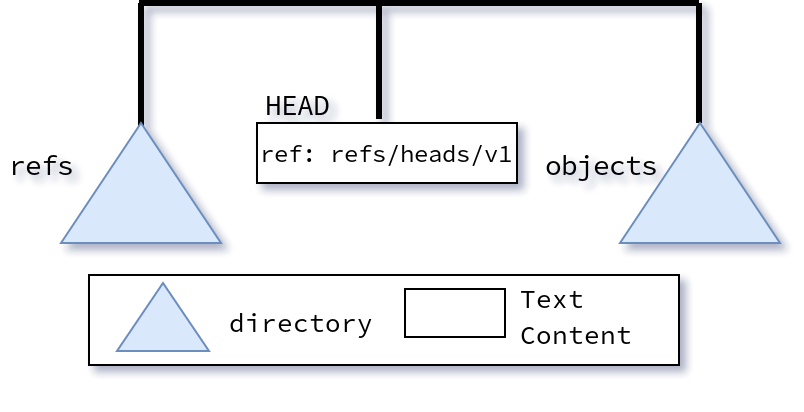
\includegraphics[width=0.75\textwidth,keepaspectratio]{./images/gitDirectory-Root.png}
            }
            {
                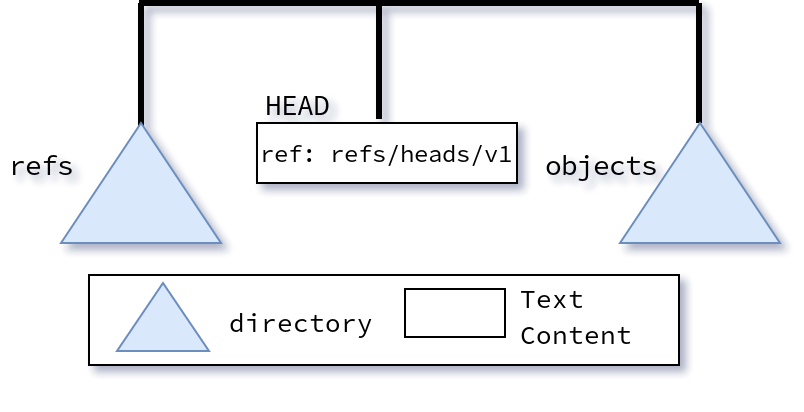
\includegraphics[height=0.75\textheight,keepaspectratio]{./images/gitDirectory-Root.png}
            }
            \caption{.git root directory}
        \end{center}
    \end{figure}
\end{frame}




    \begin{frame}[fragile]
    \frametitle{.git directory Refs}
    \begin{figure}
        \begin{center}
            \ifnumequal{\aspectratio}{43}
            {
                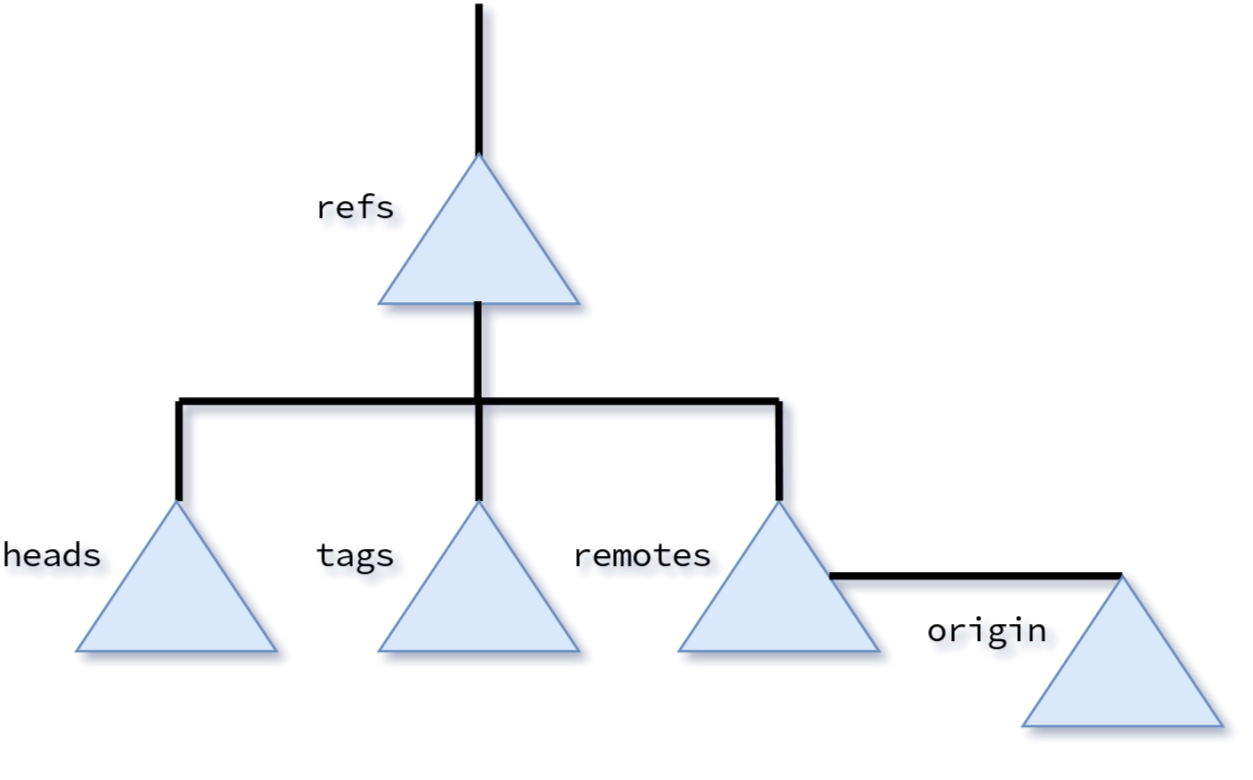
\includegraphics[height=0.75\textheight,keepaspectratio]{./images/gitDirectory-Refs.png}
            }
            {
                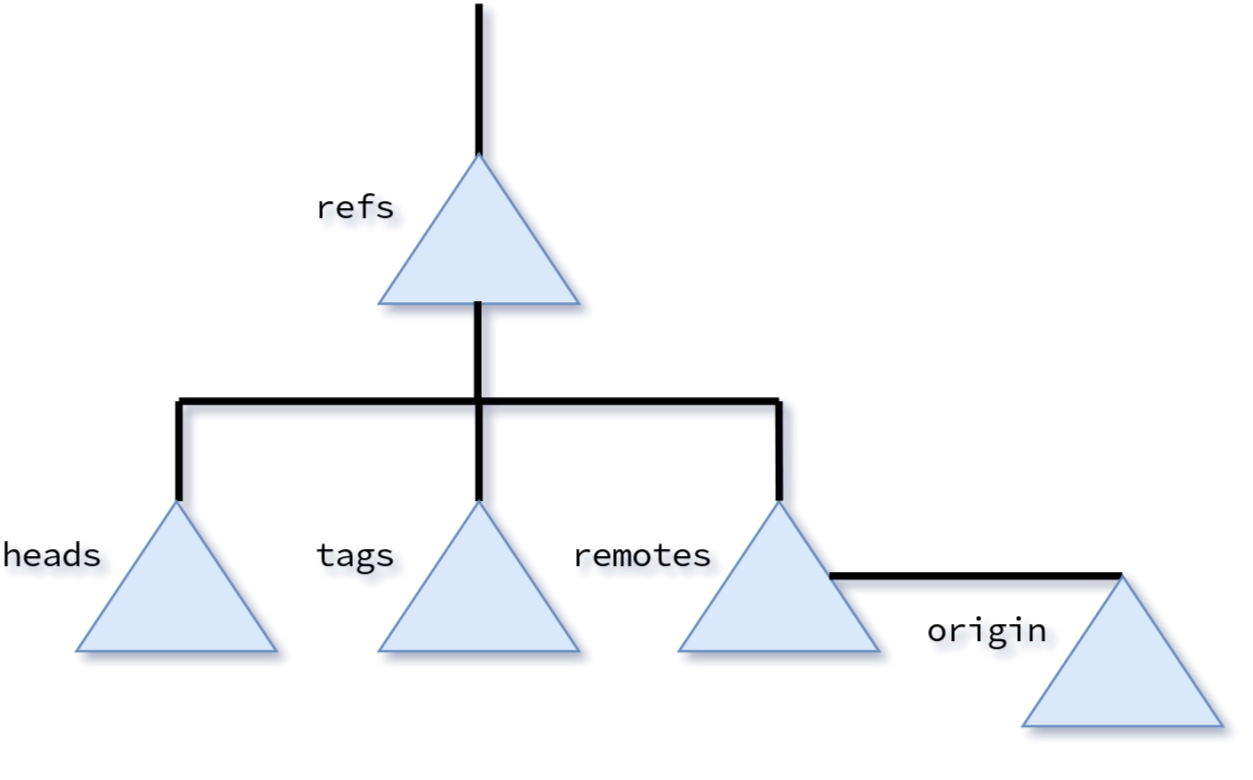
\includegraphics[height=0.75\textheight,width=0.8\textwidth]{./images/gitDirectory-Refs.png}
            }
            \caption{.git directory Refs}
        \end{center}
    \end{figure}
\end{frame}



    \begin{frame}[fragile,noframenumbering]
    \frametitle{.git directory Refs with content}
    \addtocounter{page}{-1}
    \begin{figure}
        \begin{center}
            \ifnumequal{\aspectratio}{43}
            {
                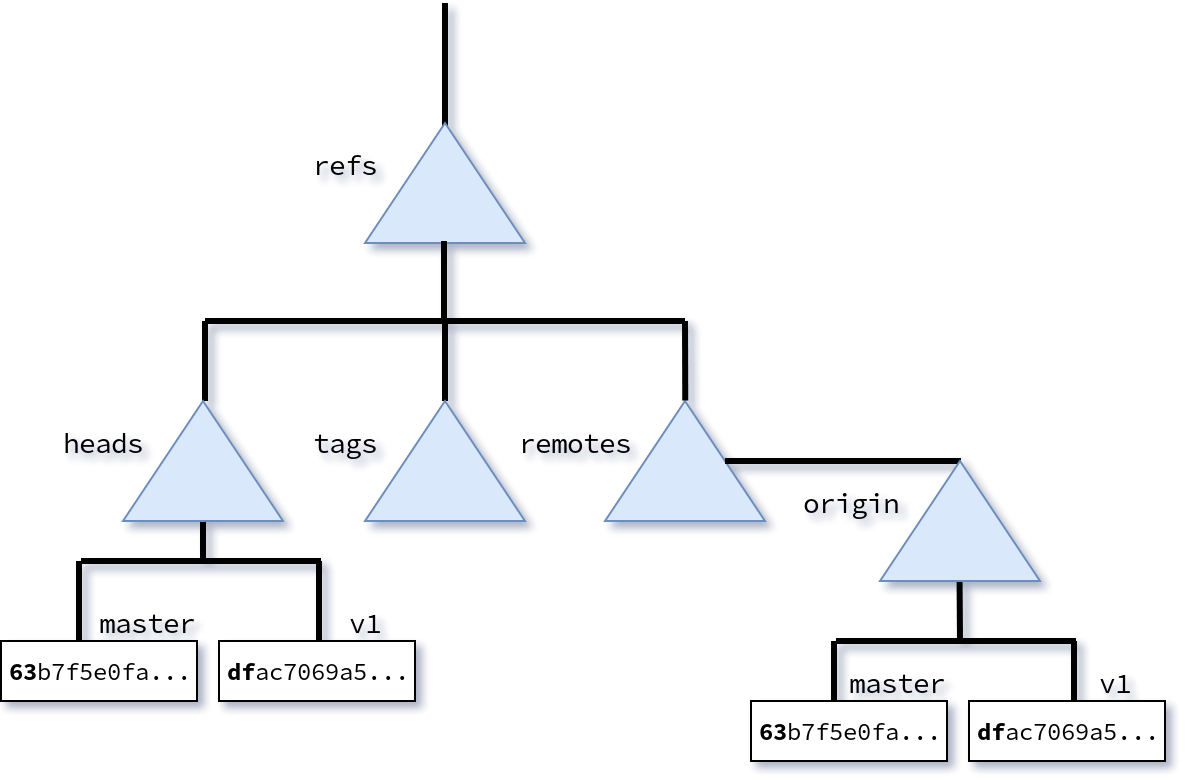
\includegraphics[height=0.75\textheight,keepaspectratio]{./images/gitDirectory-Refs_Content.png}
            }
            {
                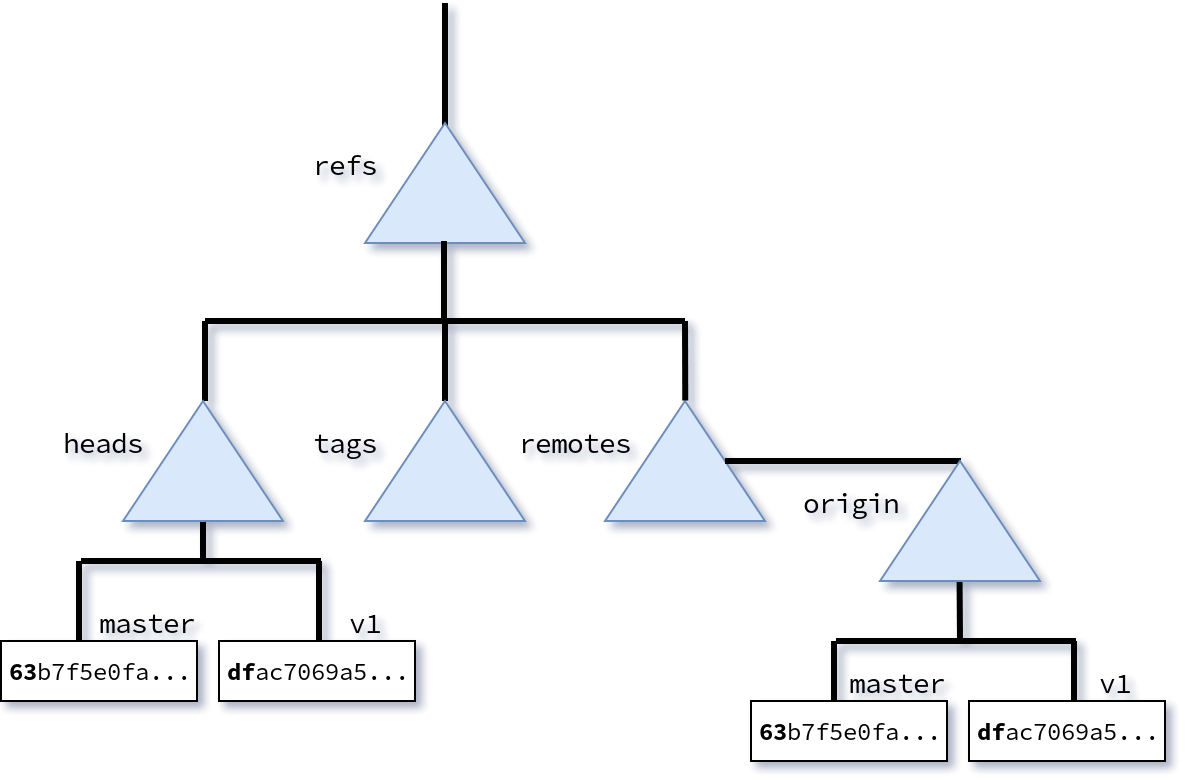
\includegraphics[height=0.75\textheight,width=0.8\textwidth]{./images/gitDirectory-Refs_Content.png}
            }
            \caption{.git directory Refs with content}
        \end{center}
    \end{figure}
\end{frame}



    \section{Contents of .git directory}
\begin{frame}[fragile]
    \frametitle{Exploring the .git directory}
    \begin{figure}
        \begin{center}
            \ifnumequal{\aspectratio}{43}
            {
                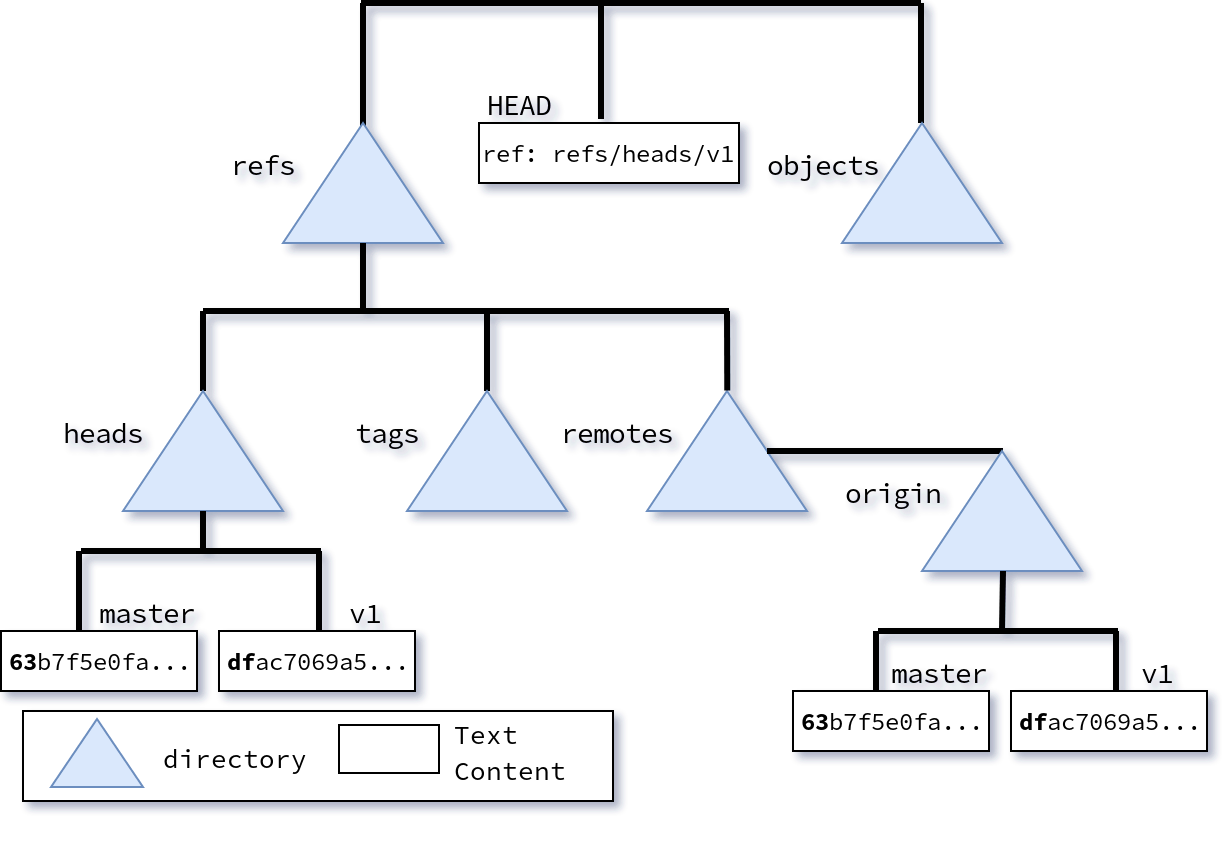
\includegraphics[height=0.75\textheight,keepaspectratio]{./images/gitDirectory.png}
            }
            {
                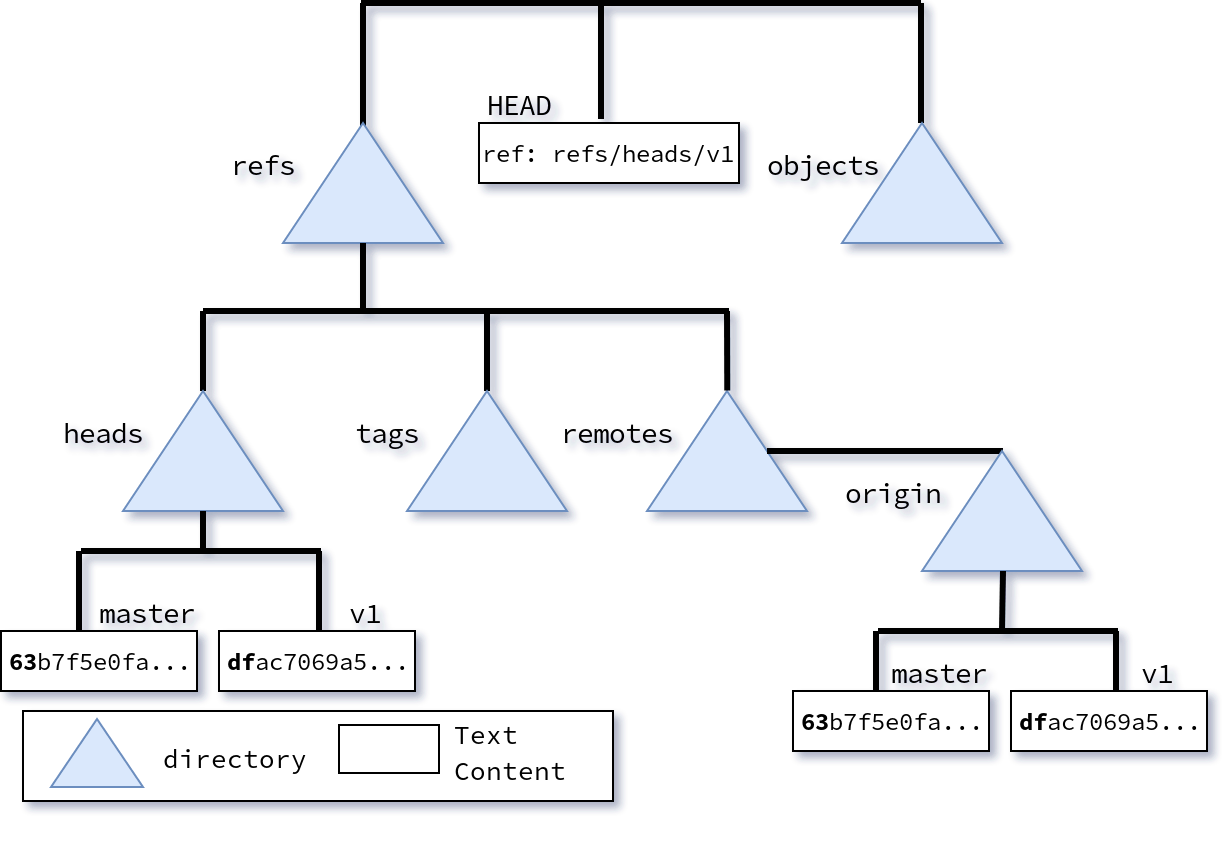
\includegraphics[height=0.75\textheight,width=0.8\textwidth]{./images/gitDirectory.png}
            }
            \caption{.git directory}
        \end{center}
    \end{figure}
\end{frame}



    \subsection{objects}
\begin{frame}[fragile]
    \frametitle{Exploring the objects directory}
    \lstset{
        language=bash,
        showstringspaces=true,
        frame=single,
        style=BashInputStyle
    }
    \begin{lstlisting}[caption={git log --raw -n1}, label={fig:lograw}]
commit d8c22f8205cab34e00e6a172febedd6d5f1a2ada (HEAD -> master)
Author: [...]
Date:   [...]

    Git directory Root added

:100644 100644 dbd87be bccdfbd M        README
:000000 100644 0000000 1b16bf9 A        images/gitDirectory-Root.png
:000000 100644 0000000 013543d A        slides/GitDirectoryRoot.tex
    \end{lstlisting}
\end{frame}

\begin{frame}[fragile]
    \frametitle{objects directory}
    \lstset{
        language=bash,
        showstringspaces=true,
        frame=single,
        style=BashInputStyle
    }
    \begin{lstlisting}[caption={[Tree]tree .git/objects example (shortened with comments)},label={fig:objectsdirectory}]
./.git/objects
|-- 87
|   |-- ccb1974b8bbcb39aa6c6bedc13a27bd4308142 tree
|-- bc
|   |-- cdfbd6314e19a21c367ba5ea9cbe65a1a0818e blob
|-- d2
|   |-- e82a9df8b4521fb6b25f22fb87ffe0e873413c staged blob
|-- d8
|   |-- c22f8205cab34e00e6a172febedd6d5f1a2ada commit
|-- info
|-- pack
    \end{lstlisting}
\end{frame}



    \subsection{Treeish}
\begin{frame}
    \frametitle{Treeish objects}
    \begin{figure}
        \begin{center}
            \ifnumequal{\aspectratio}{43}
            {
                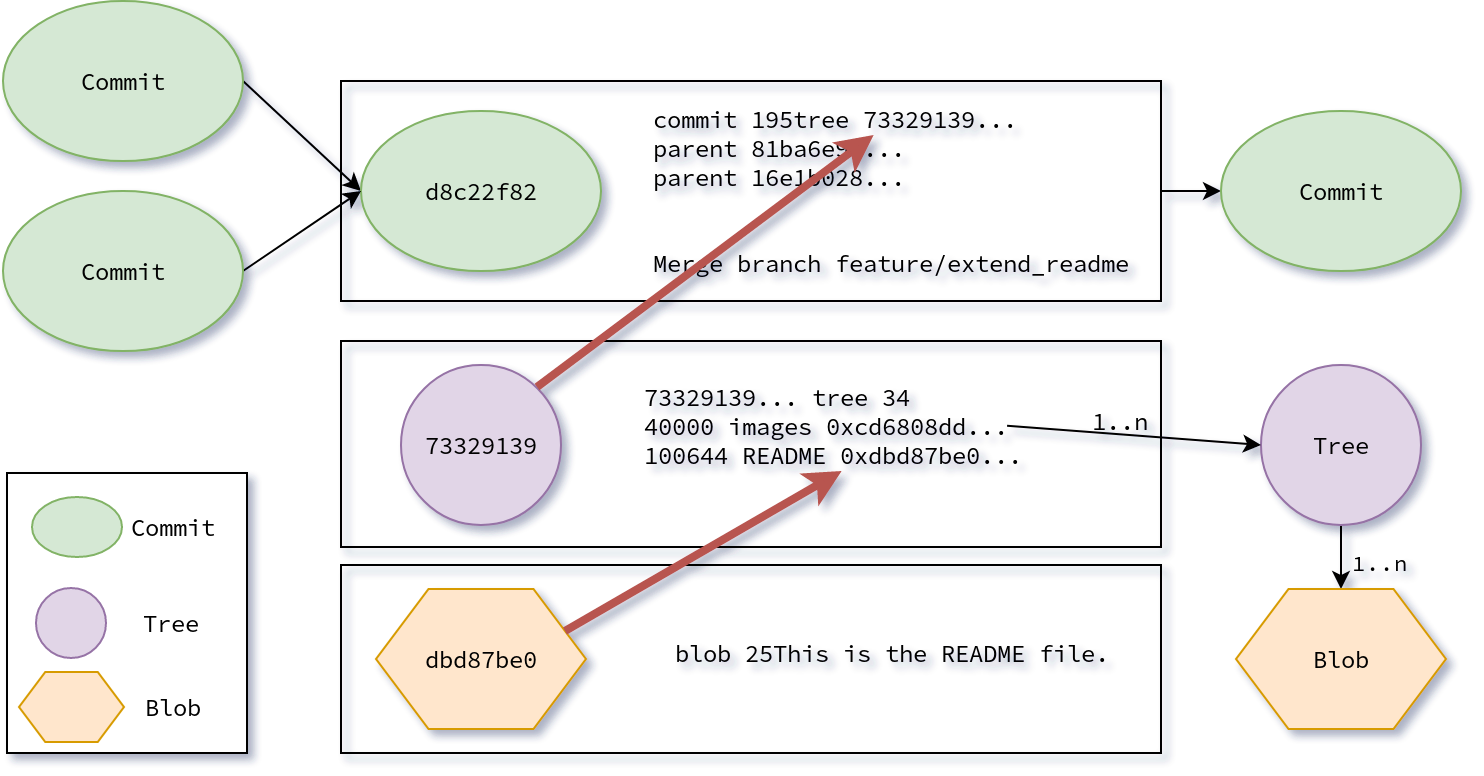
\includegraphics[height=0.70\textheight,keepaspectratio]{./images/Treeish.png}
            }
            {
                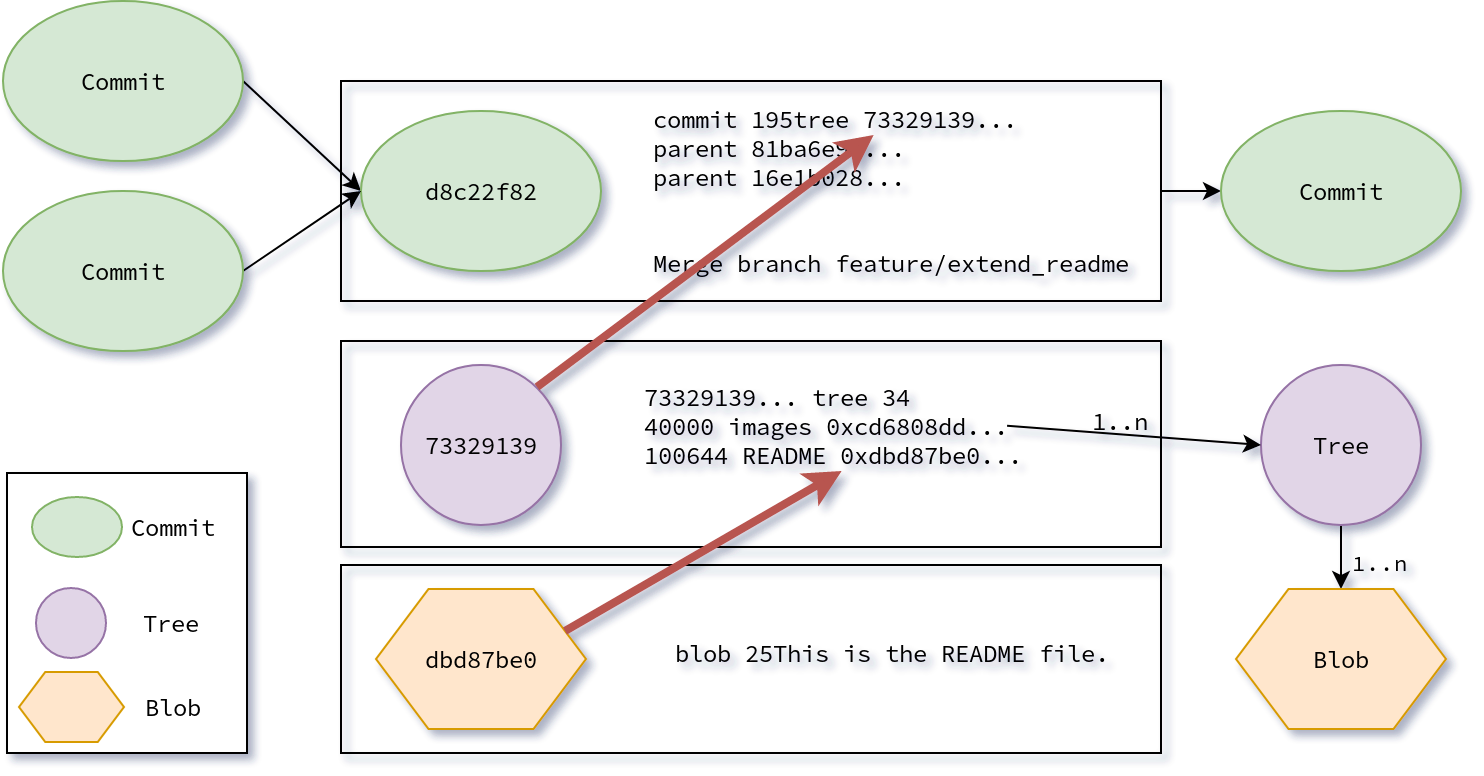
\includegraphics[height=0.6\textheight,width=0.8\textwidth]{./images/Treeish.png}
            }
            \caption{Git tree object explained}
        \end{center}
    \end{figure}
\end{frame}

\begin{frame}[noframenumbering]
    \frametitle{Treeish objects - commit}
    \addtocounter{page}{-1}
    \begin{figure}
        \begin{center}
            \ifnumequal{\aspectratio}{43}
            {
                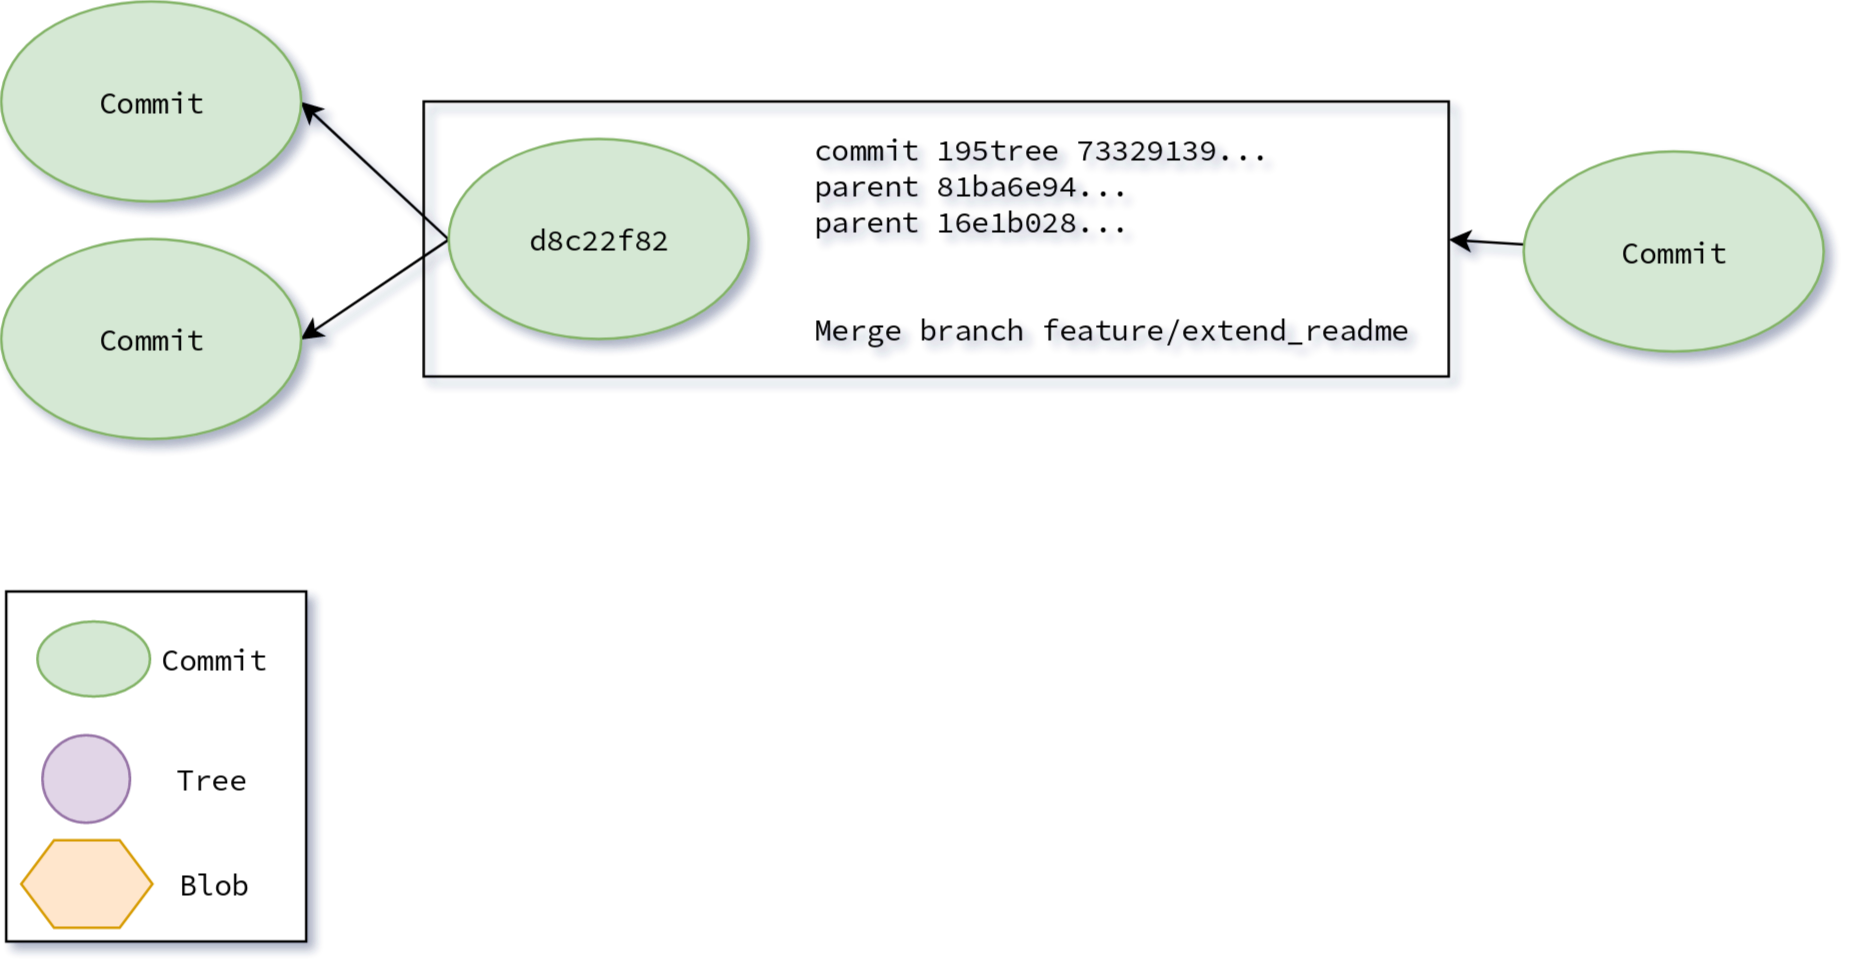
\includegraphics[height=0.70\textheight,keepaspectratio]{./images/Treeish_Commit.png}
            }
            {
                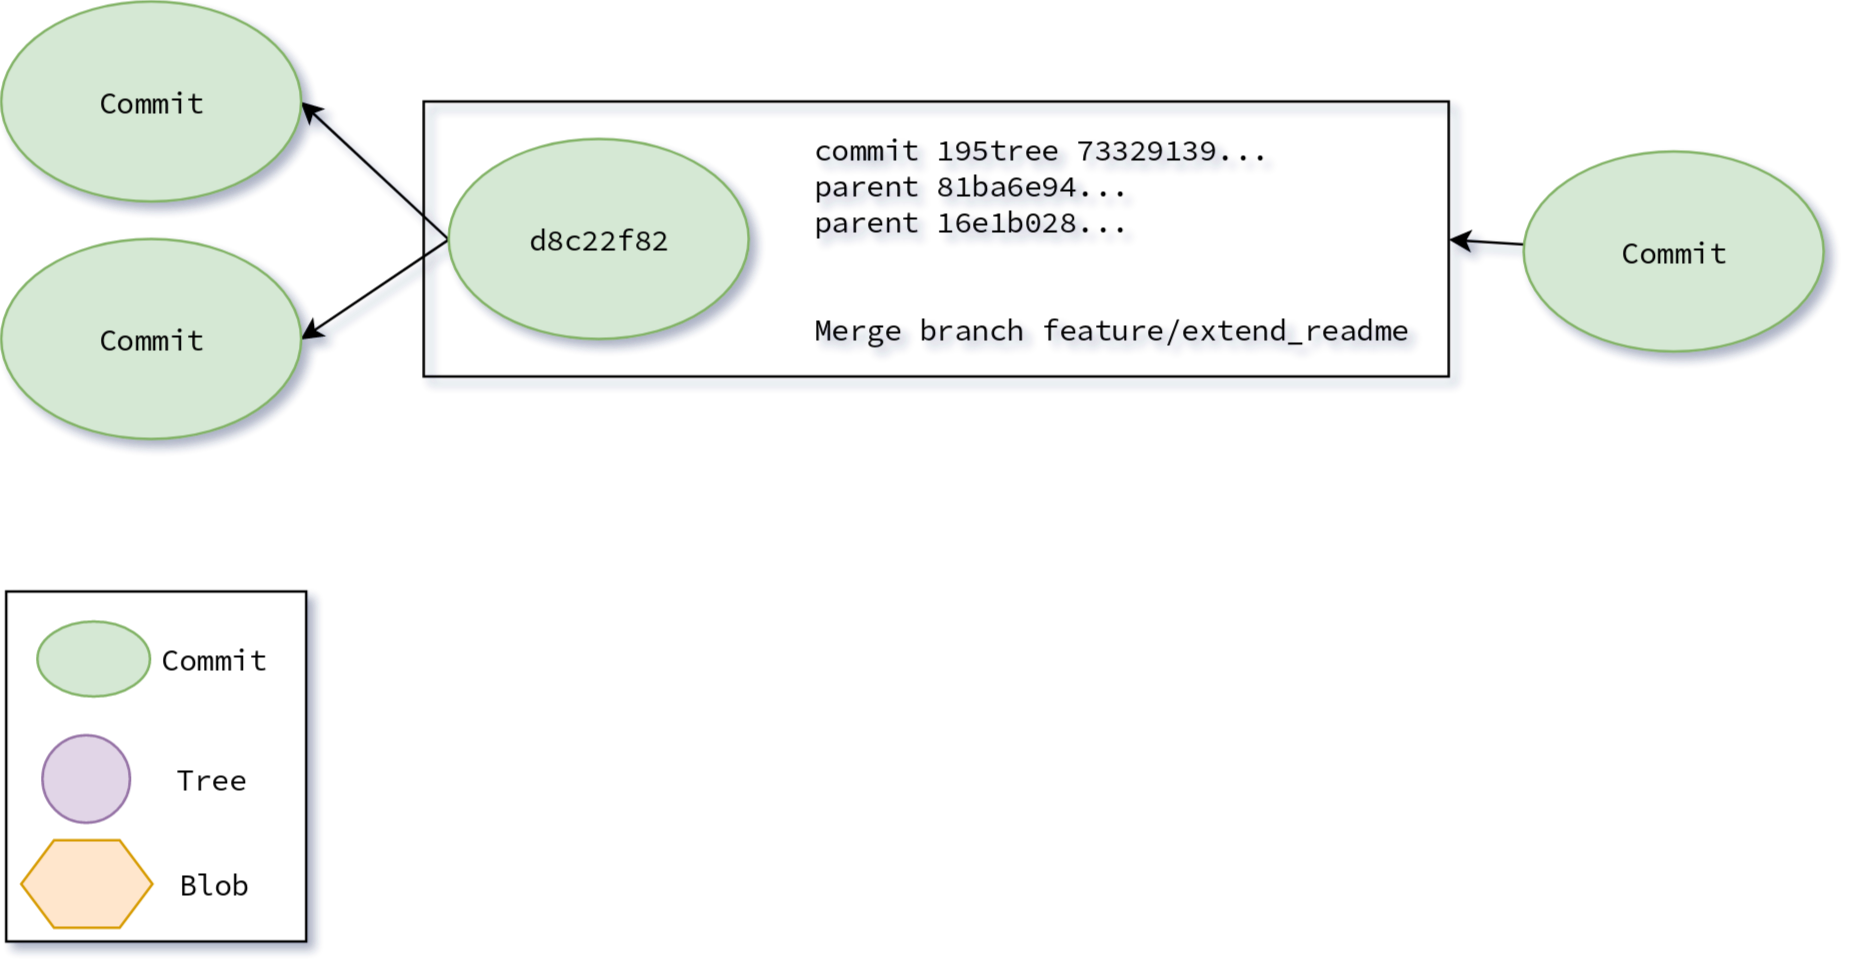
\includegraphics[height=0.6\textheight,width=0.8\textwidth]{./images/Treeish_Commit.png}
            }
            \caption{Git commit}
        \end{center}
    \end{figure}
\end{frame}

\begin{frame}[noframenumbering]
    \frametitle{Treeish objects - tree}
    \addtocounter{page}{-1}
    \begin{figure}
        \begin{center}
            \ifnumequal{\aspectratio}{43}
            {
                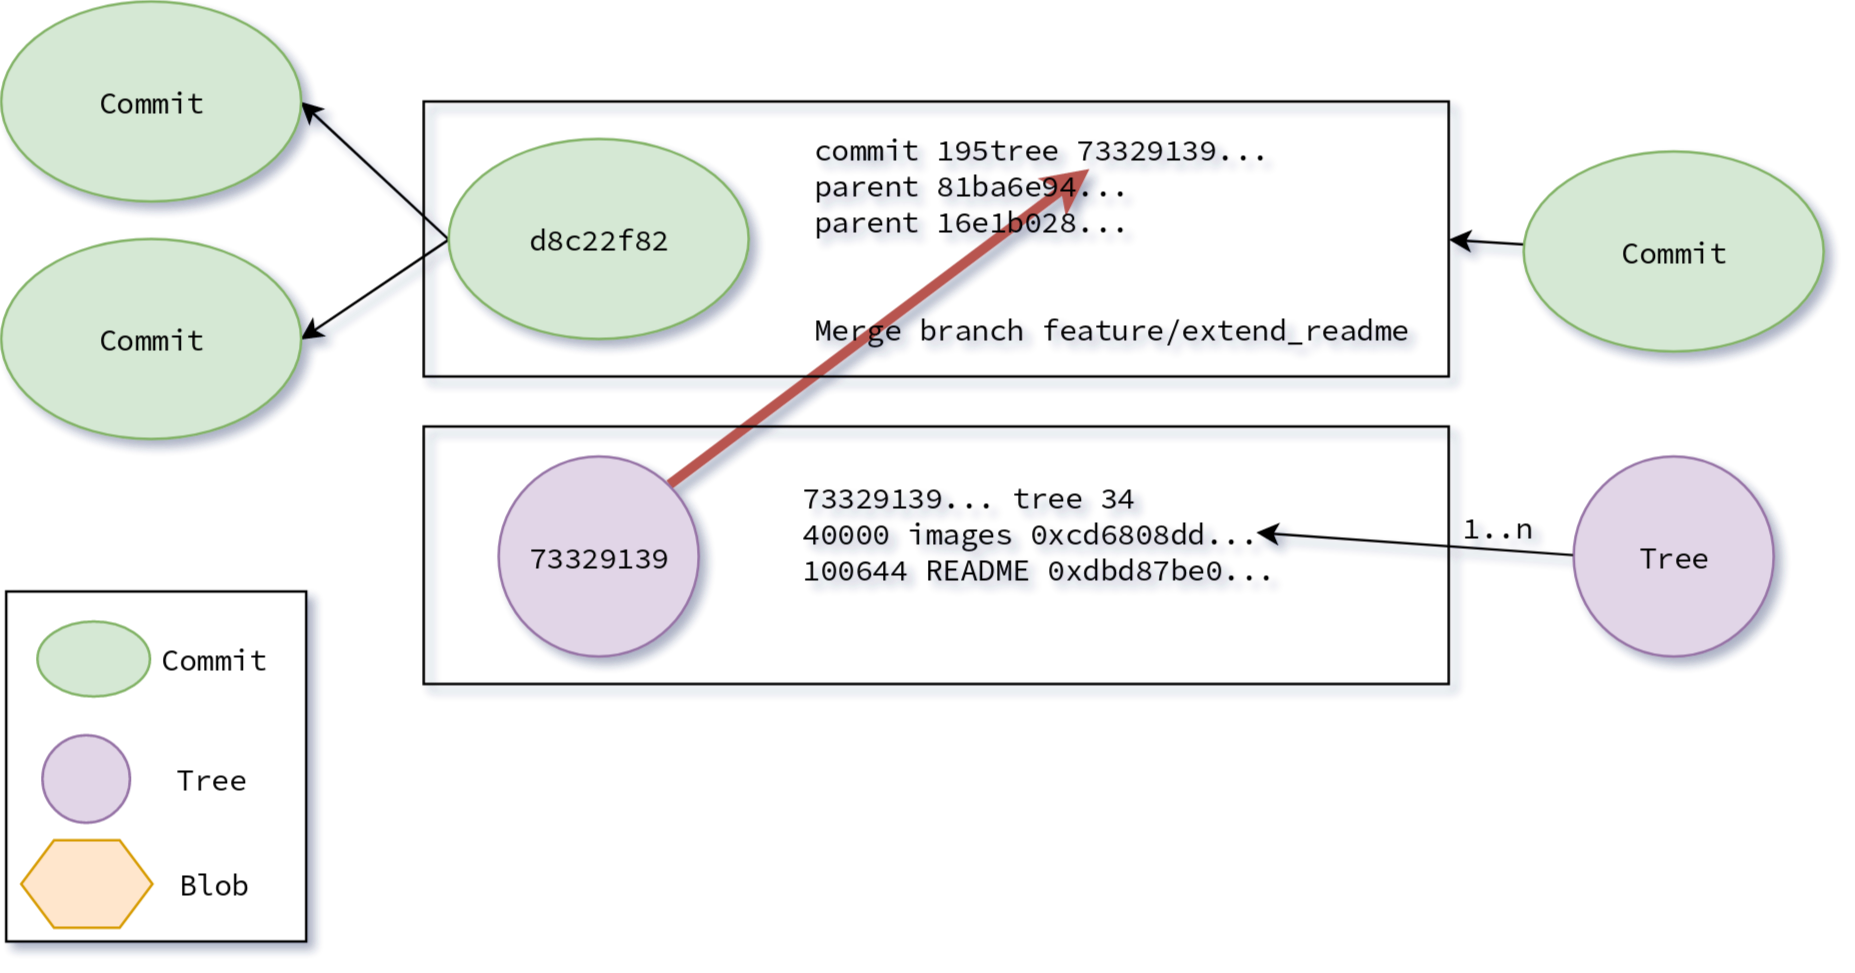
\includegraphics[height=0.70\textheight,keepaspectratio]{./images/Treeish_Tree.png}
            }
            {
                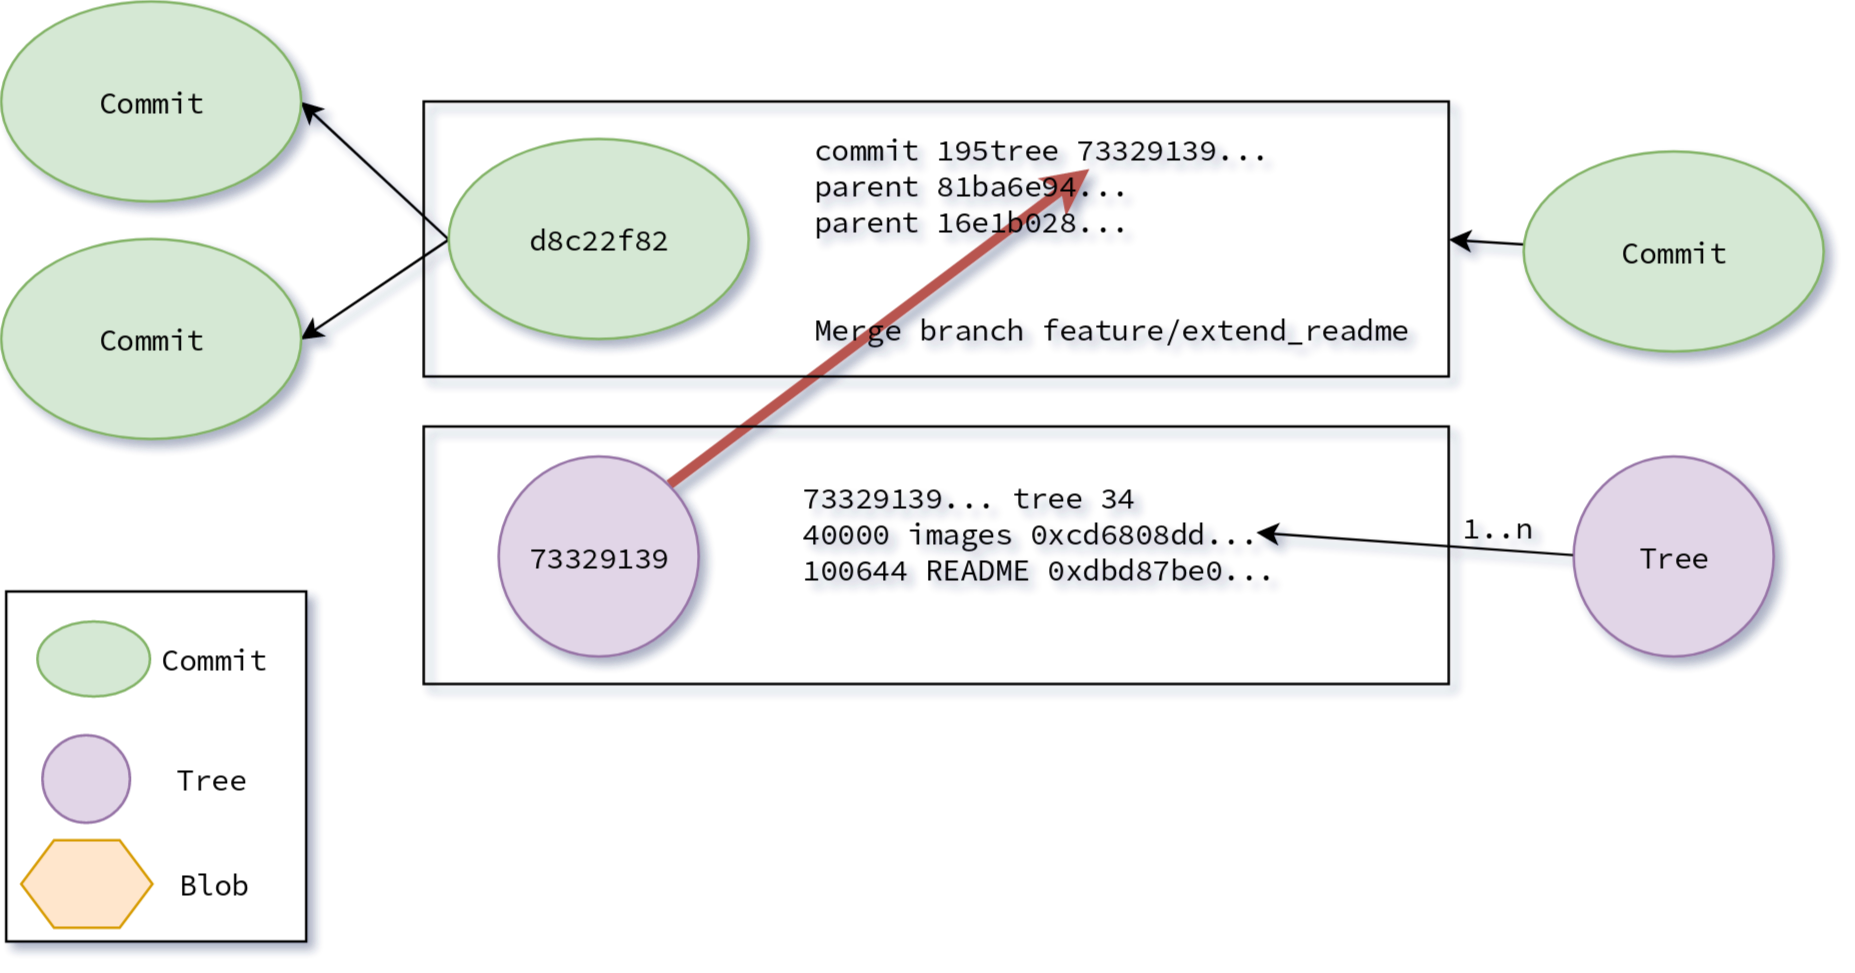
\includegraphics[height=0.6\textheight,width=0.8\textwidth]{./images/Treeish_Tree.png}
            }
            \caption{Git tree}
        \end{center}
    \end{figure}
\end{frame}

\begin{frame}[noframenumbering]
    \frametitle{Treeish objects - blob}
    \addtocounter{page}{-1}
    \begin{figure}
        \begin{center}
            \ifnumequal{\aspectratio}{43}
            {
                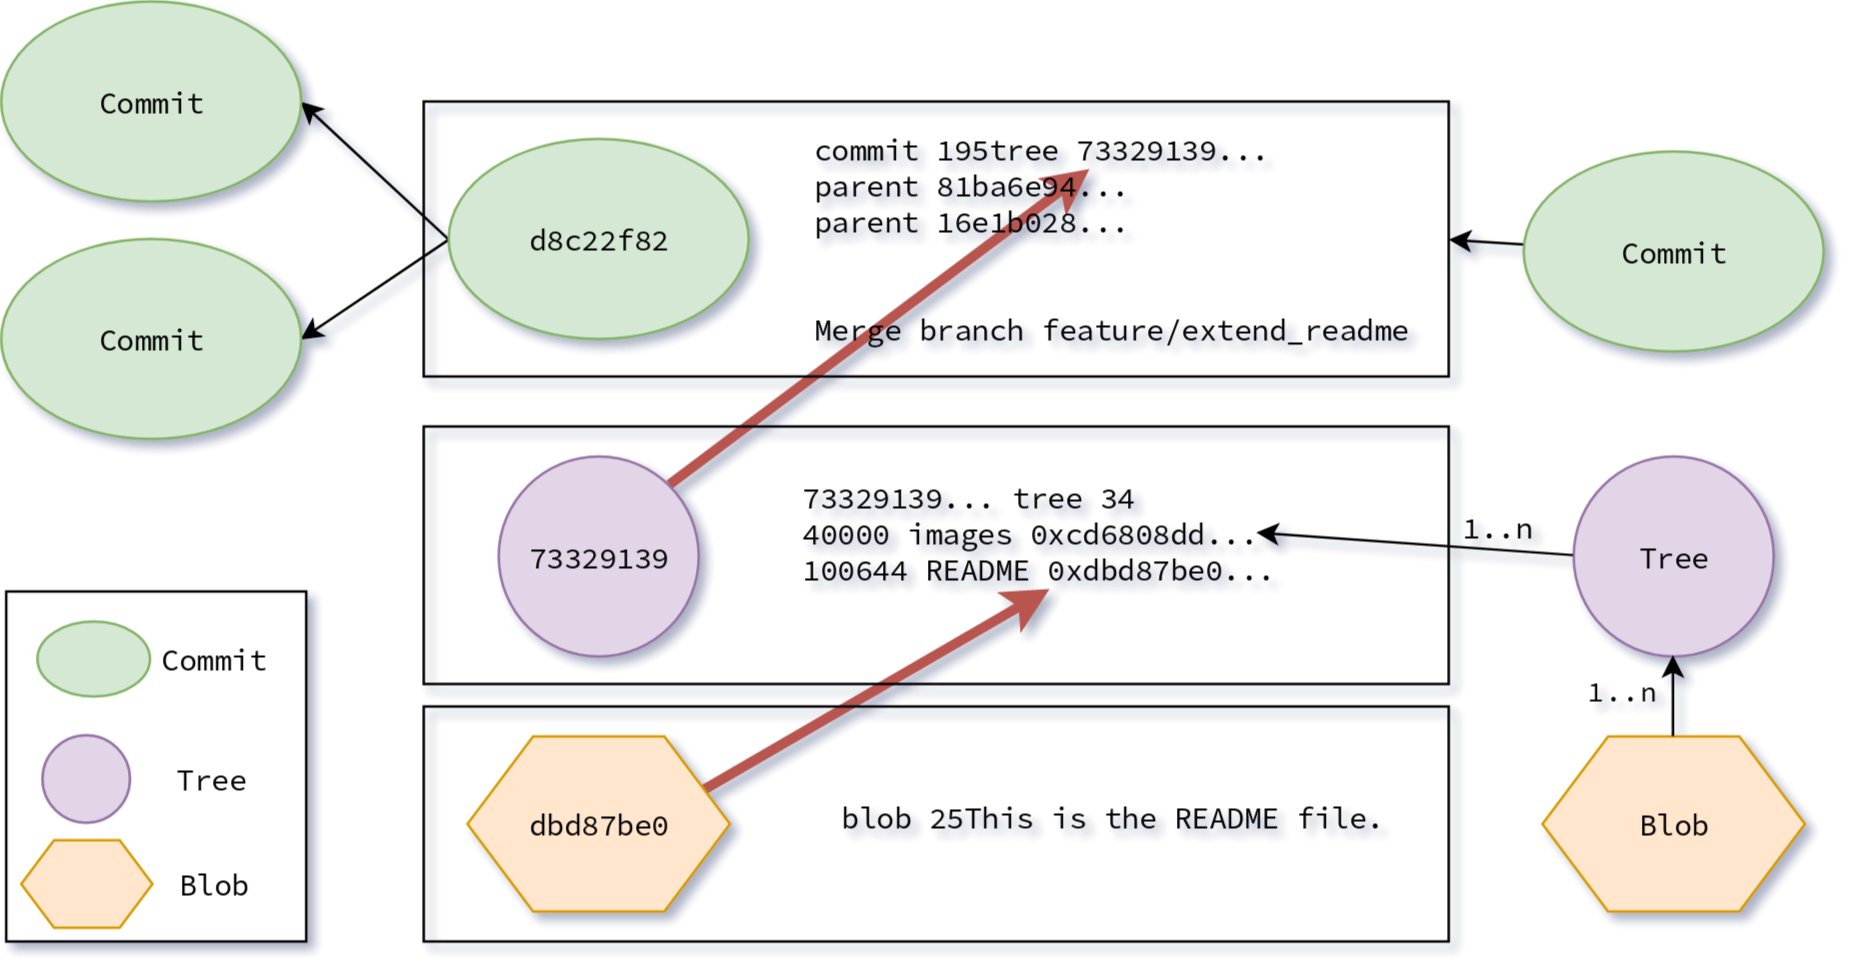
\includegraphics[height=0.70\textheight,keepaspectratio]{./images/Treeish_Blob.png}
            }
            {
                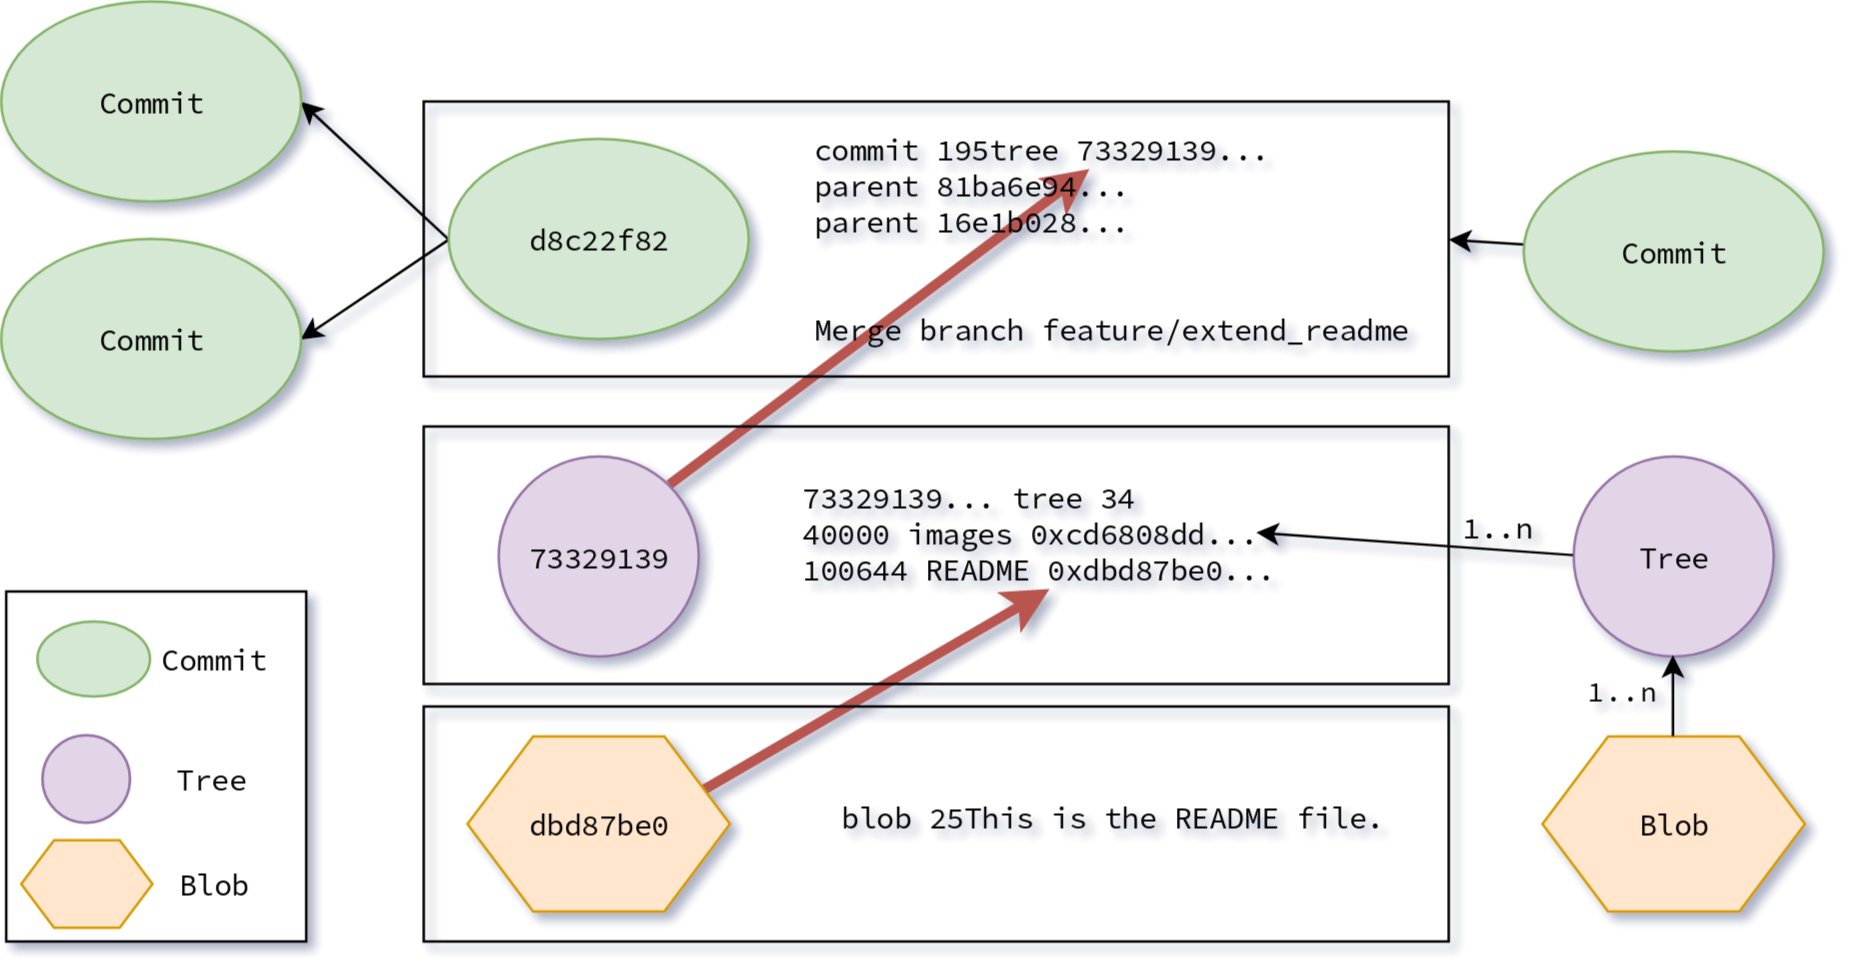
\includegraphics[height=0.6\textheight,width=0.8\textwidth]{./images/Treeish_Blob.png}
            }
            \caption{Git blob}
        \end{center}
    \end{figure}
\end{frame}



    \subsection{Recap}
\begin{frame}
    \frametitle{Recap .git directory}
    \begin{itemize}
        \item All files of git are stored in the hidden directory
        \item Commits, Trees and Blobs are referenced by their sha1\footnotemark
        \footnotetext{
            \href
                {https://tools.ietf.org/html/rfc6234}
                {RFC 6234}
        }
        \item Commits hold a reference to the tree of the root directory of the repository
        \item The history of commits is a directed acyclic graph\footnotemark
        \footnotetext{
            \href
                {https://eagain.net/articles/git-for-computer-scientists}
                {git for computer scientists}
        }
        \item Trees reference directories of the project
        \item The root directory of the repository is always a tree object
        \item Blobs are the file contents of that specific point in the history
    \end{itemize}
\end{frame}



    \section{Git areas}
\subsection{The stages of Git}
\begin{frame}[fragile]
    \frametitle{Different areas in git}
    \begin{figure}
        \begin{center}
            \ifnumequal{\aspectratio}{43}
            {
                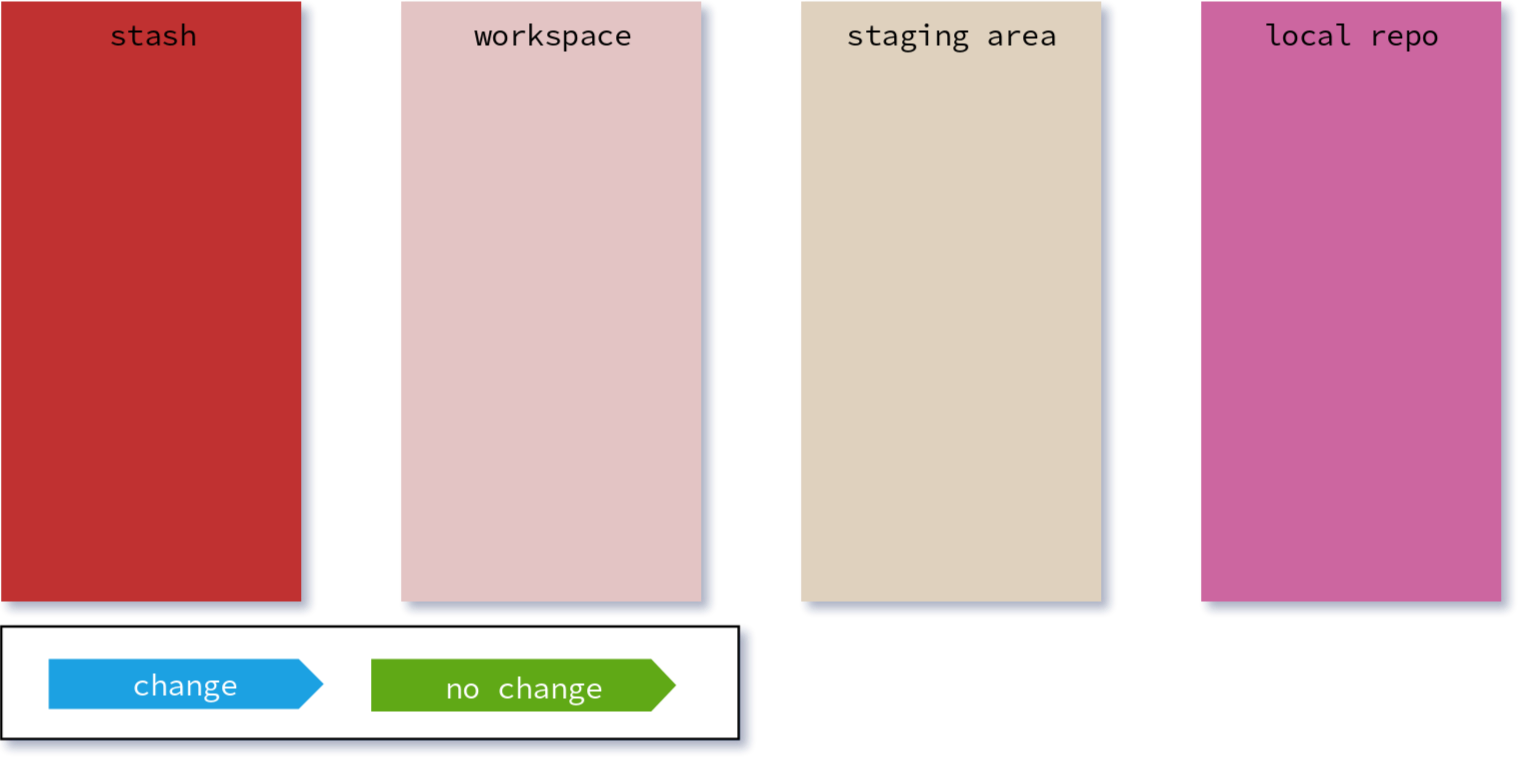
\includegraphics[width=1\textwidth,keepaspectratio]{./images/GitAreas.png}
            }
            {
                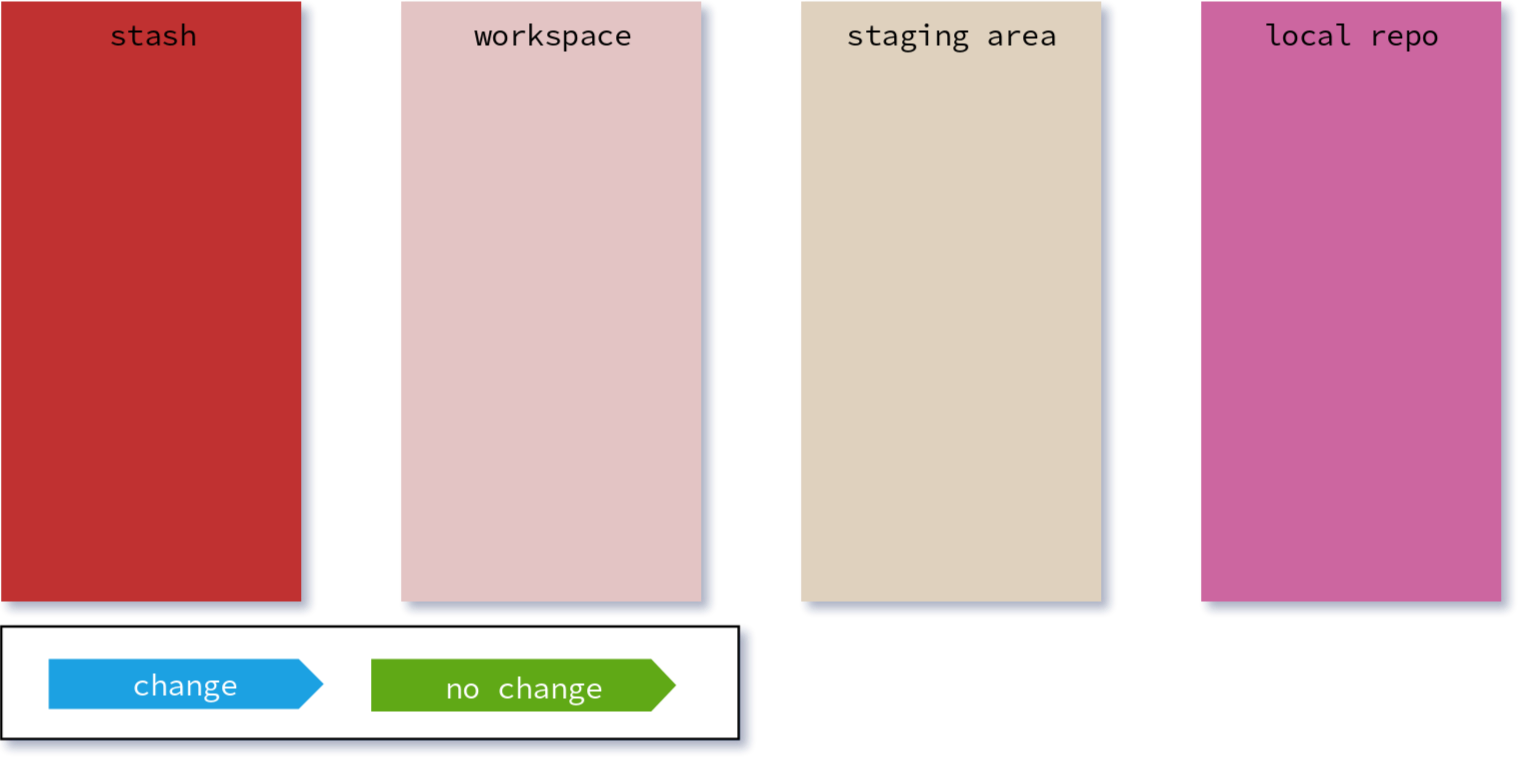
\includegraphics[height=0.75\textheight,keepaspectratio]{./images/GitAreas.png}
            }
            \caption{Areas in git}
        \end{center}
    \end{figure}
\end{frame}

\subsection*{Git workspace}
\begin{frame}[fragile]
    \frametitle{Git Workspace}
    \begin{figure}
        \begin{center}
            \ifnumequal{\aspectratio}{43}
            {
                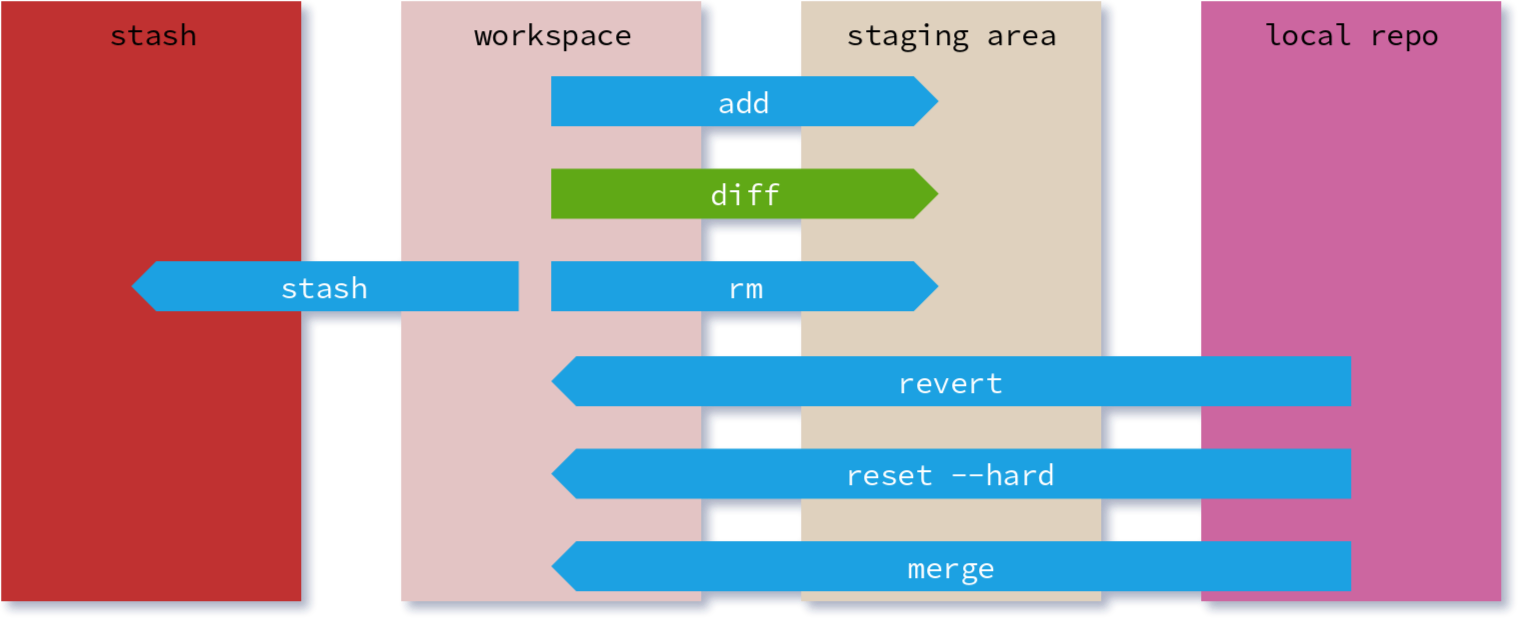
\includegraphics[width=1\textwidth,keepaspectratio]{./images/GitAreas-Workspace.png}
            }
            {
                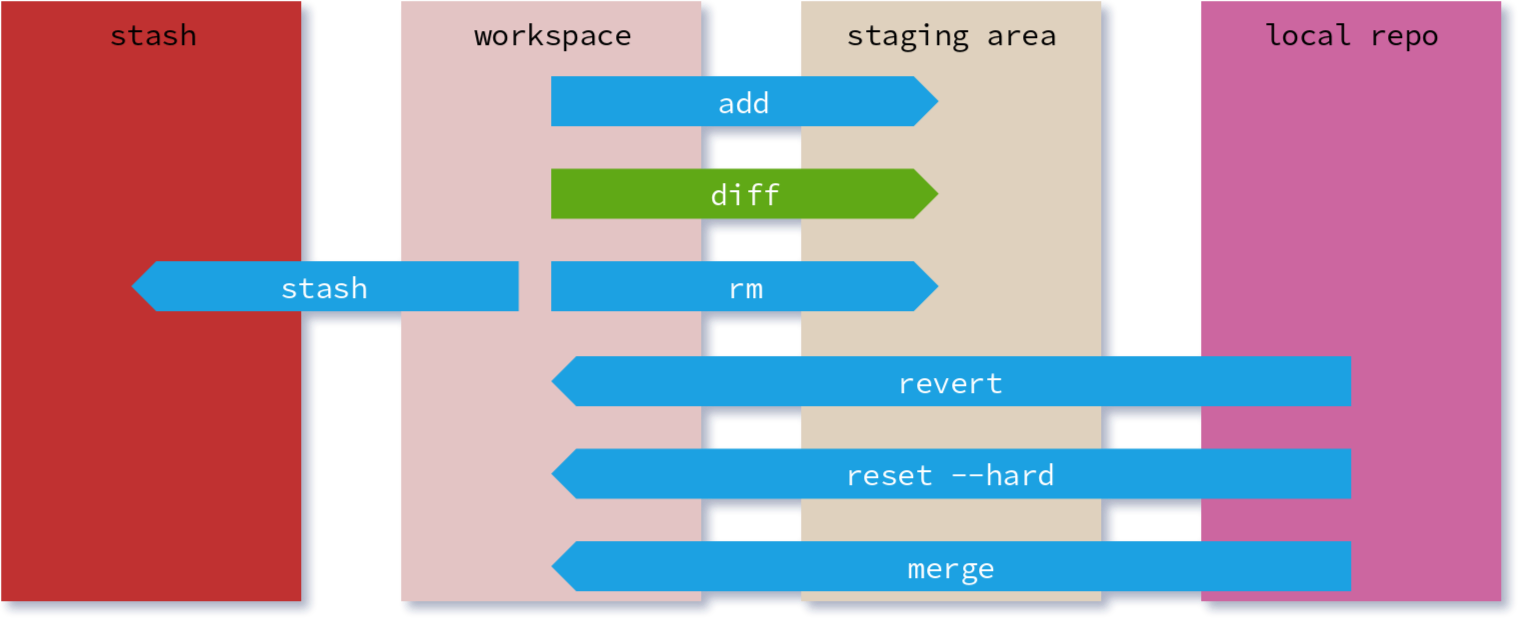
\includegraphics[height=0.75\textheight,keepaspectratio]{./images/GitAreas-Workspace.png}
            }
            \caption{Workspace area}
        \end{center}
    \end{figure}
\end{frame}

\subsection*{Git staging}
\begin{frame}[fragile]
    \frametitle{Git Staging}
    \begin{figure}
        \begin{center}
            \ifnumequal{\aspectratio}{43}
            {
                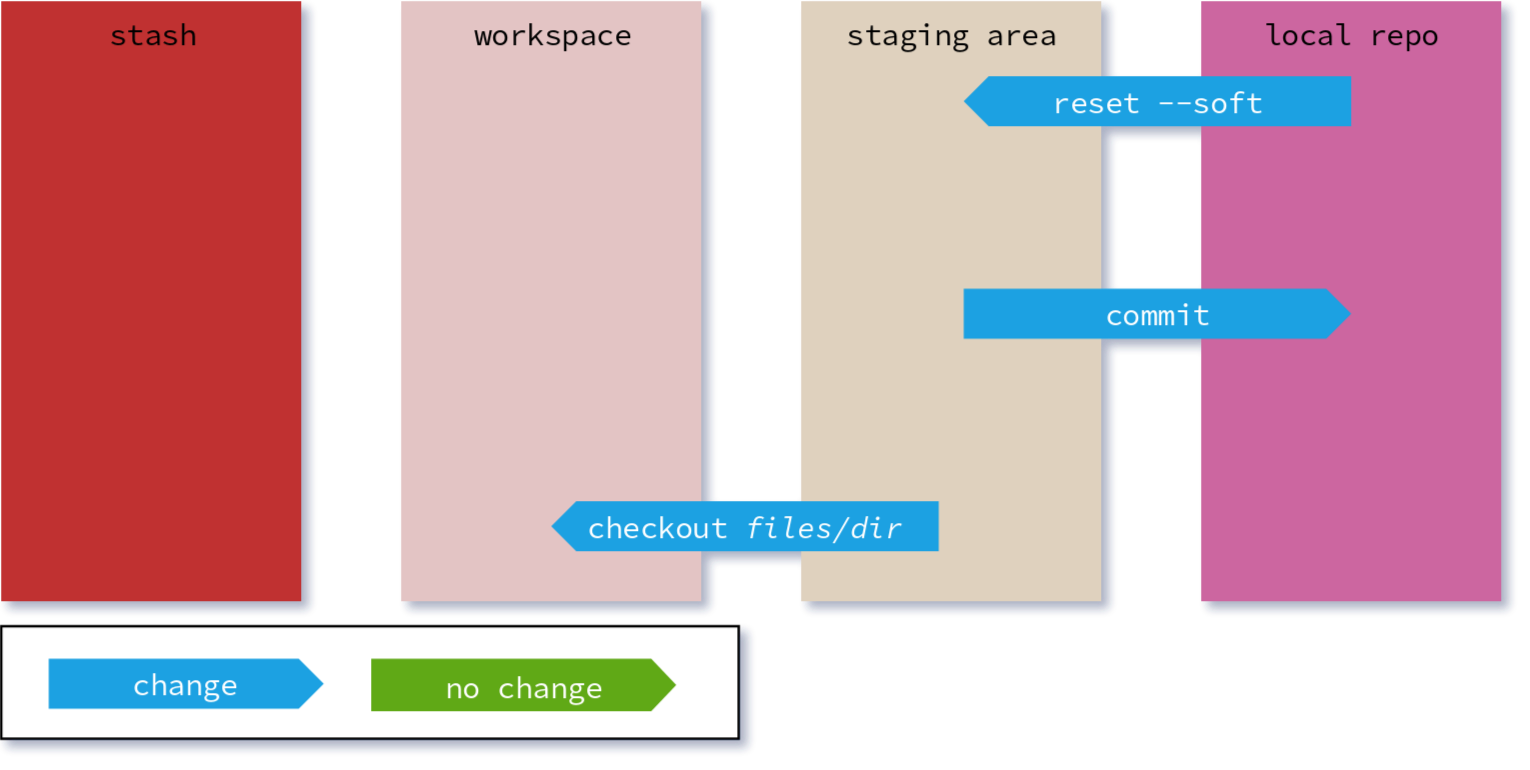
\includegraphics[width=1\textwidth,keepaspectratio]{./images/GitAreas-Staging.png}
            }
            {
                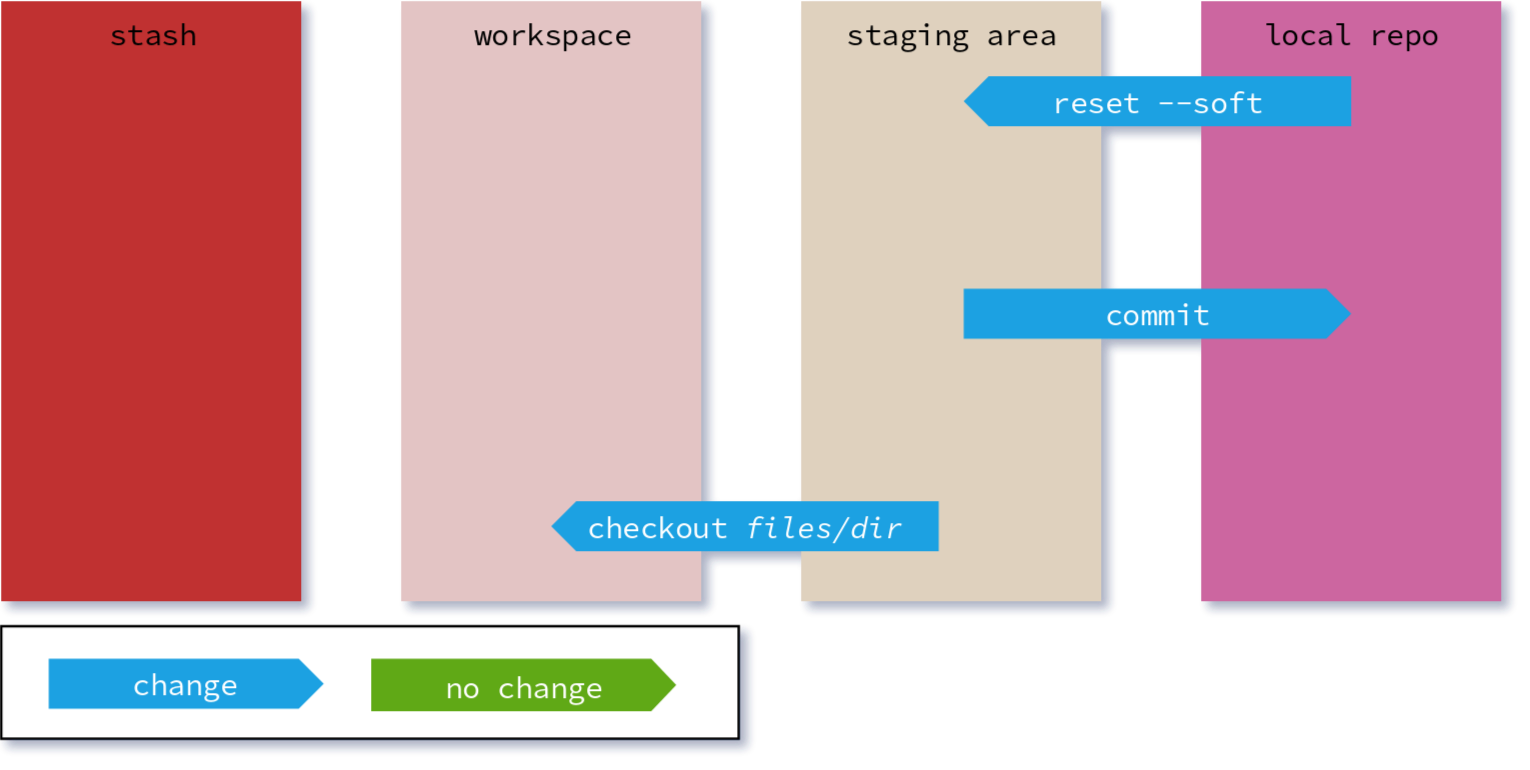
\includegraphics[height=0.75\textheight,keepaspectratio]{./images/GitAreas-Staging.png}
            }
            \caption{Staging area}
        \end{center}
    \end{figure}
\end{frame}

\subsection*{Git local repository}
\begin{frame}[fragile]
    \frametitle{Git local repository}
    \begin{figure}
        \begin{center}
            \ifnumequal{\aspectratio}{43}
            {
                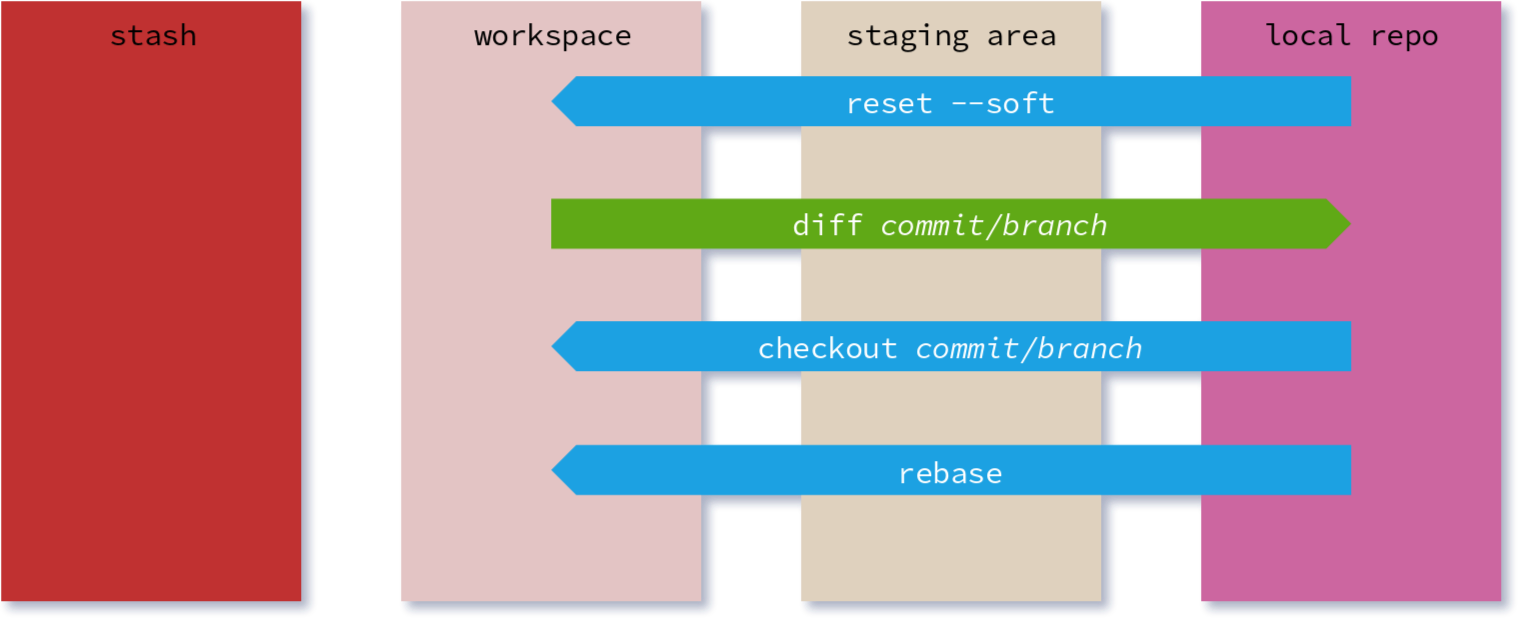
\includegraphics[width=1\textwidth,keepaspectratio]{./images/GitAreas-LocalRepo.png}
            }
            {
                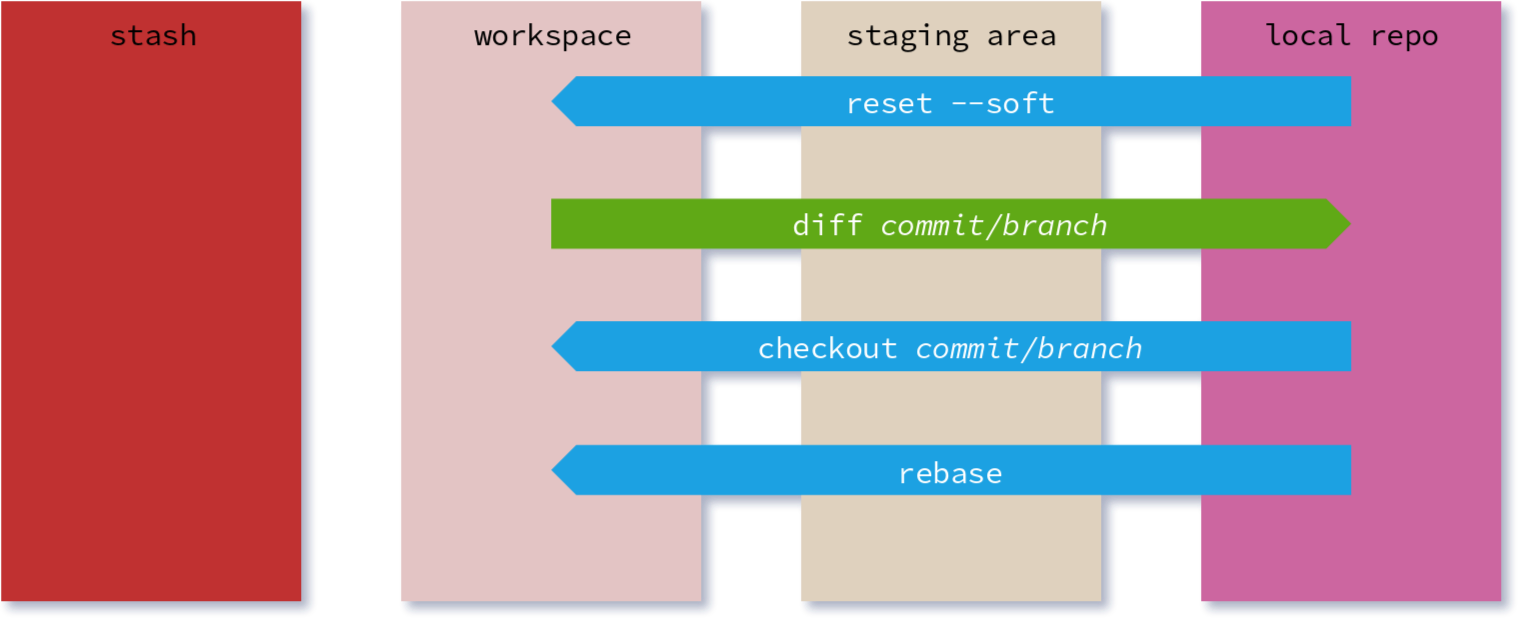
\includegraphics[height=0.75\textheight,keepaspectratio]{./images/GitAreas-LocalRepo.png}
            }
            \caption{Local repository area}
        \end{center}
    \end{figure}
\end{frame}



    \subsection{Recap}
\begin{frame}
    \frametitle{Recap Git areas}
    \begin{itemize}
        \item Three areas where you mainly work
            \begin{itemize}
                \item workspace
                \item staging also called index
                \item local repository
            \end{itemize}
        \item Most commands move changes between those areas
    \end{itemize}
\end{frame}




    \section{Git email}
\begin{frame}
    \frametitle{Git email}
    \begin{figure}
        \begin{center}
            \ifnumequal{\aspectratio}{43}
            {
                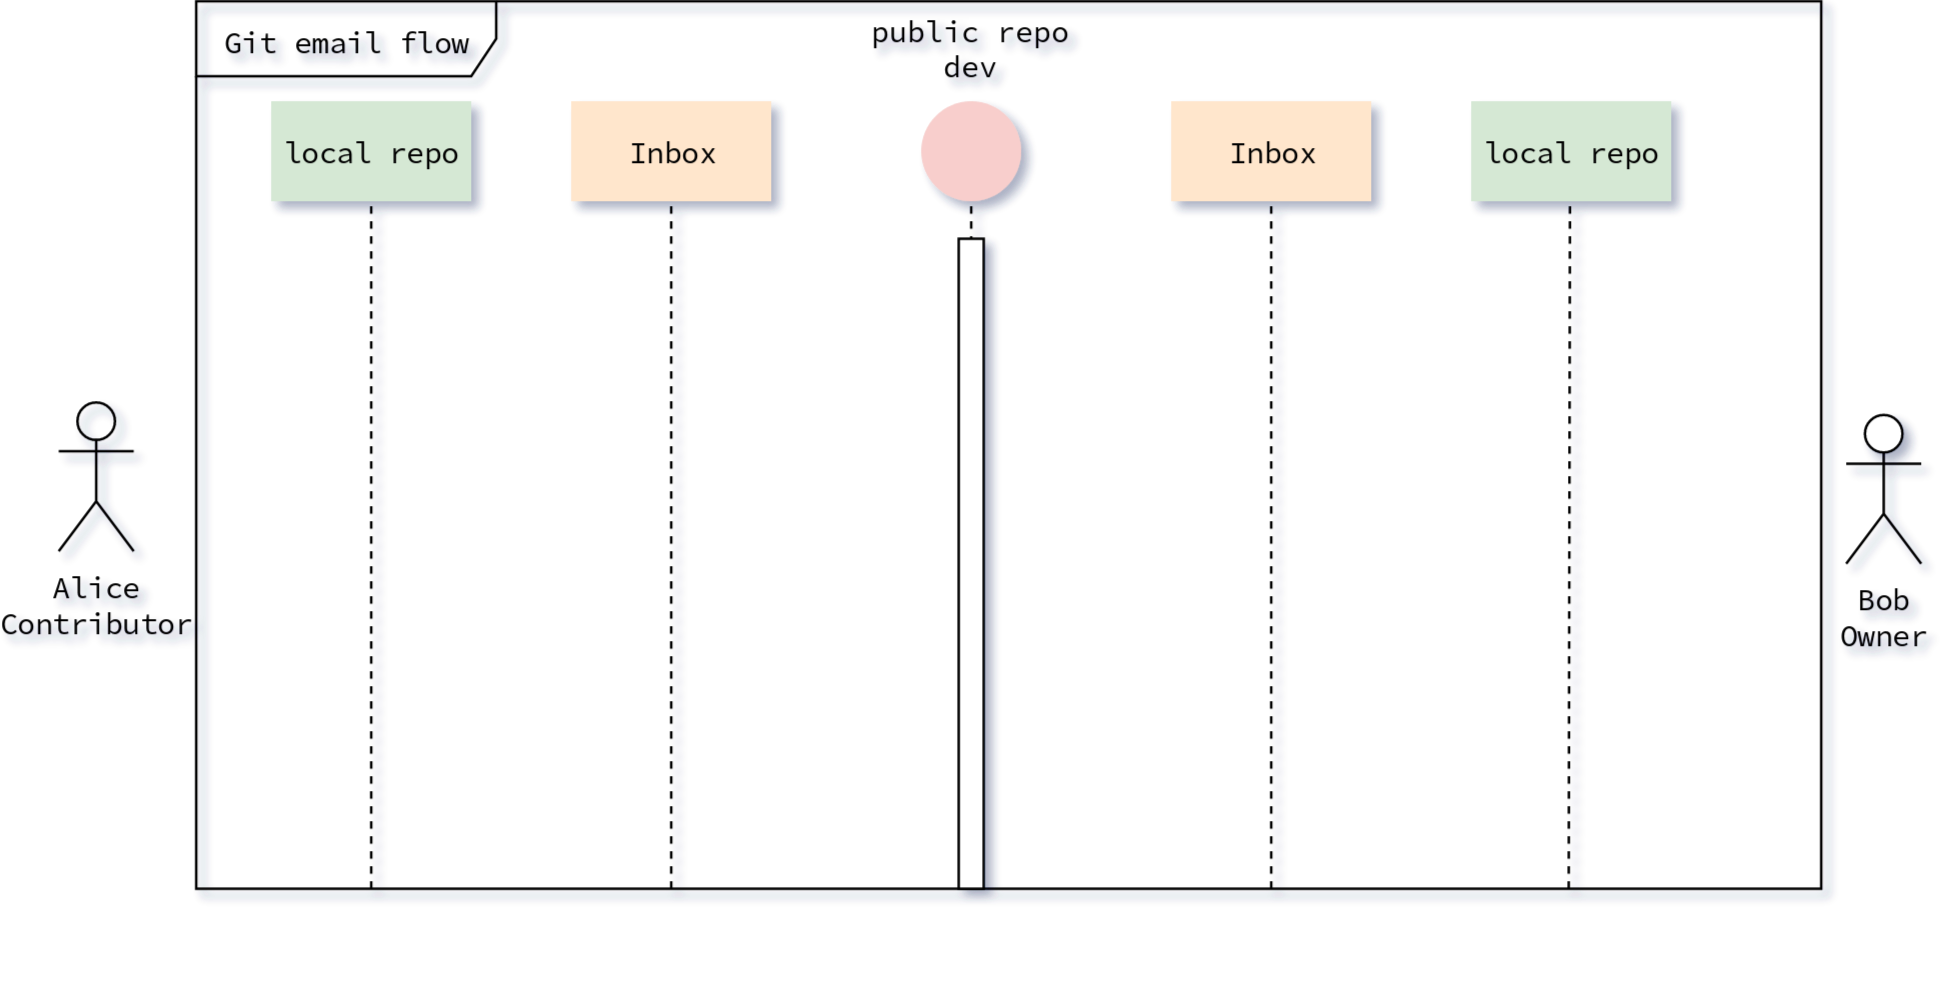
\includegraphics[height=0.7\textheight,keepaspectratio]{./images/EmailWorkflow.png}
            }
            {
                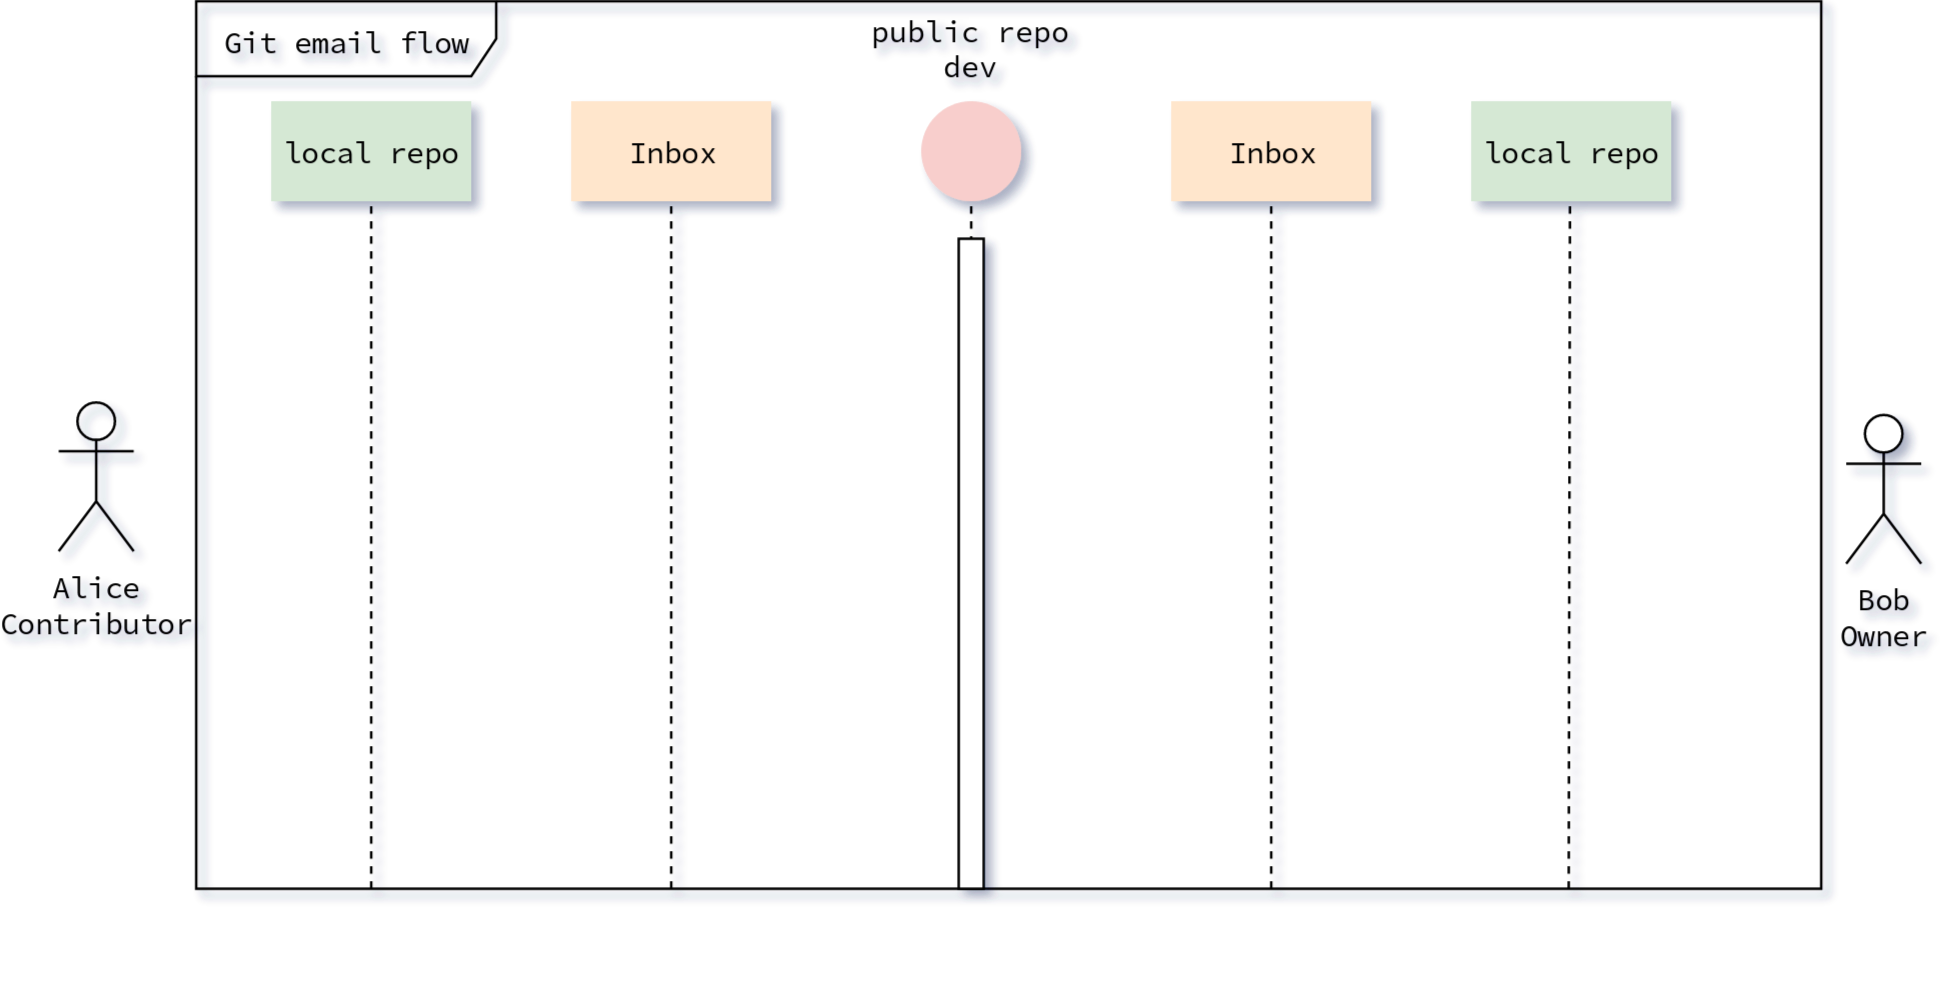
\includegraphics[height=0.75\textheight,keepaspectratio]{./images/EmailWorkflow.png}
            }
            \caption{Email workflow}
        \end{center}
    \end{figure}
\end{frame}

\begin{frame}
    \frametitle{Git email}
    \begin{figure}
        \begin{center}
            \ifnumequal{\aspectratio}{43}
            {
                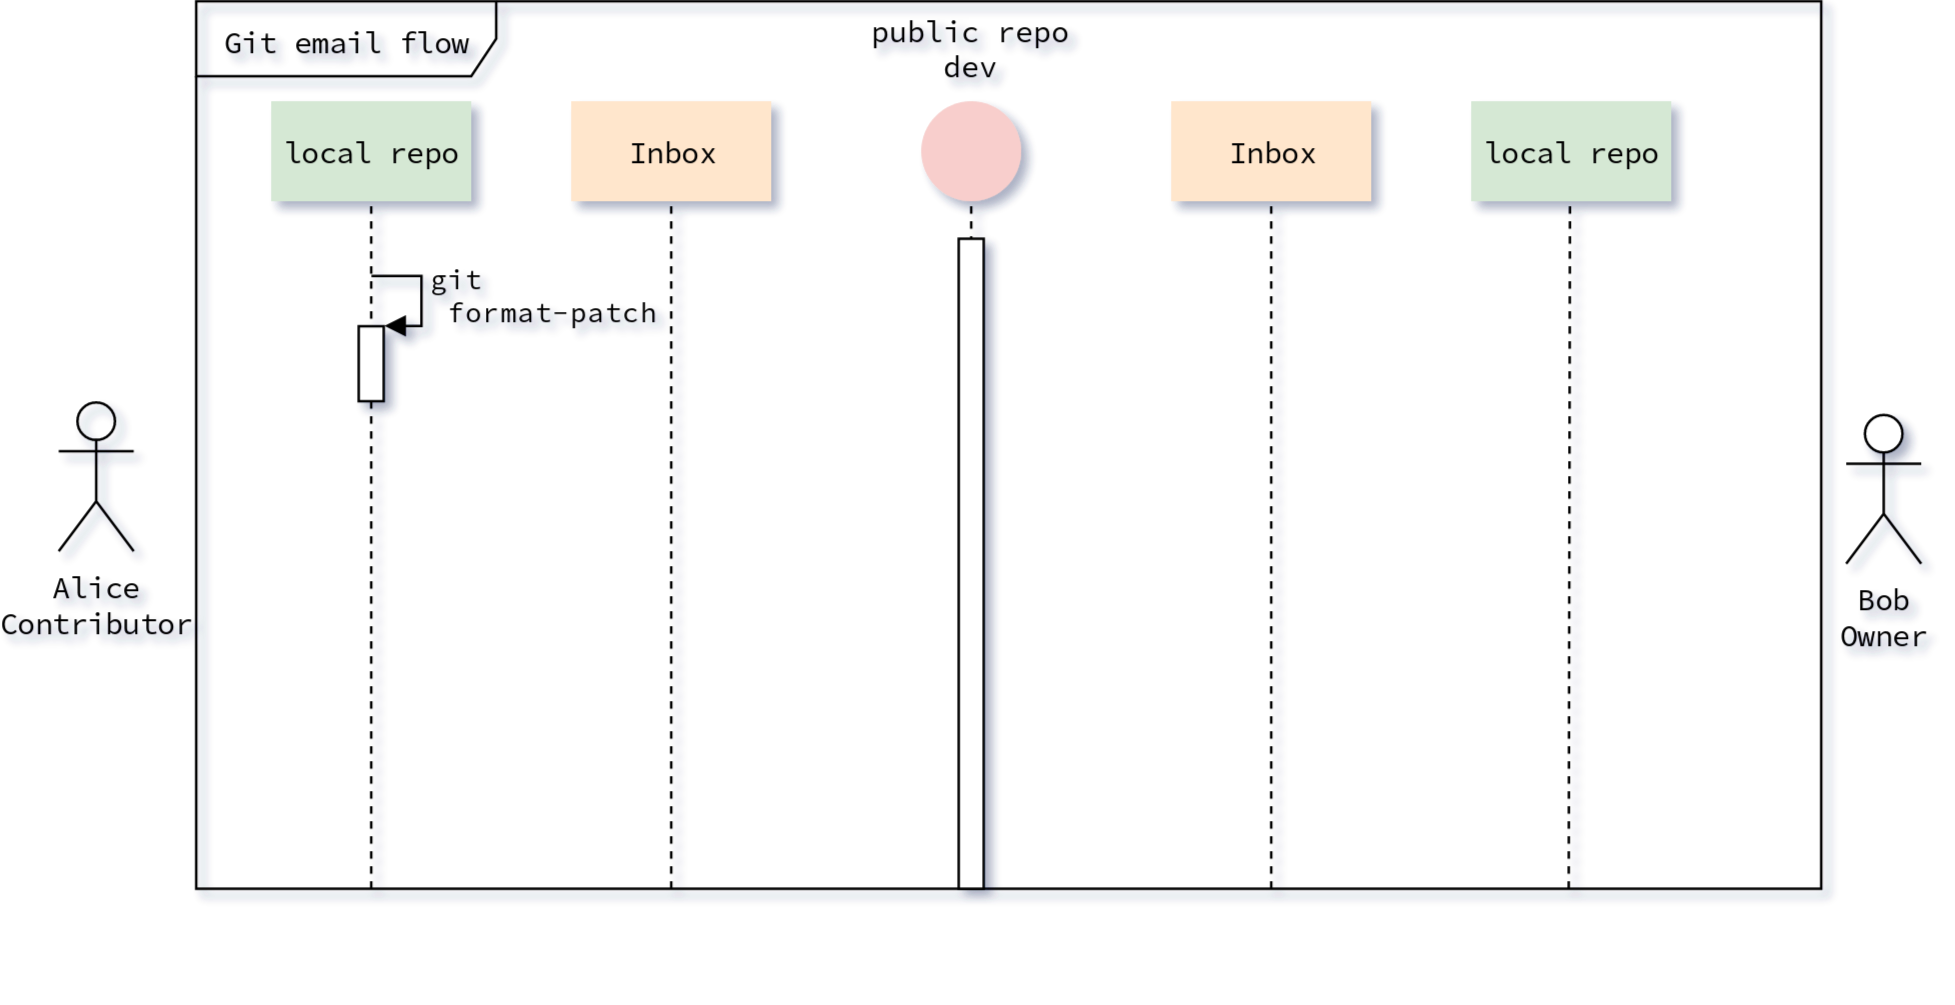
\includegraphics[height=0.7\textheight,keepaspectratio]{./images/EmailWorkflow_PrepareFirstPatch.png}
            }
            {
                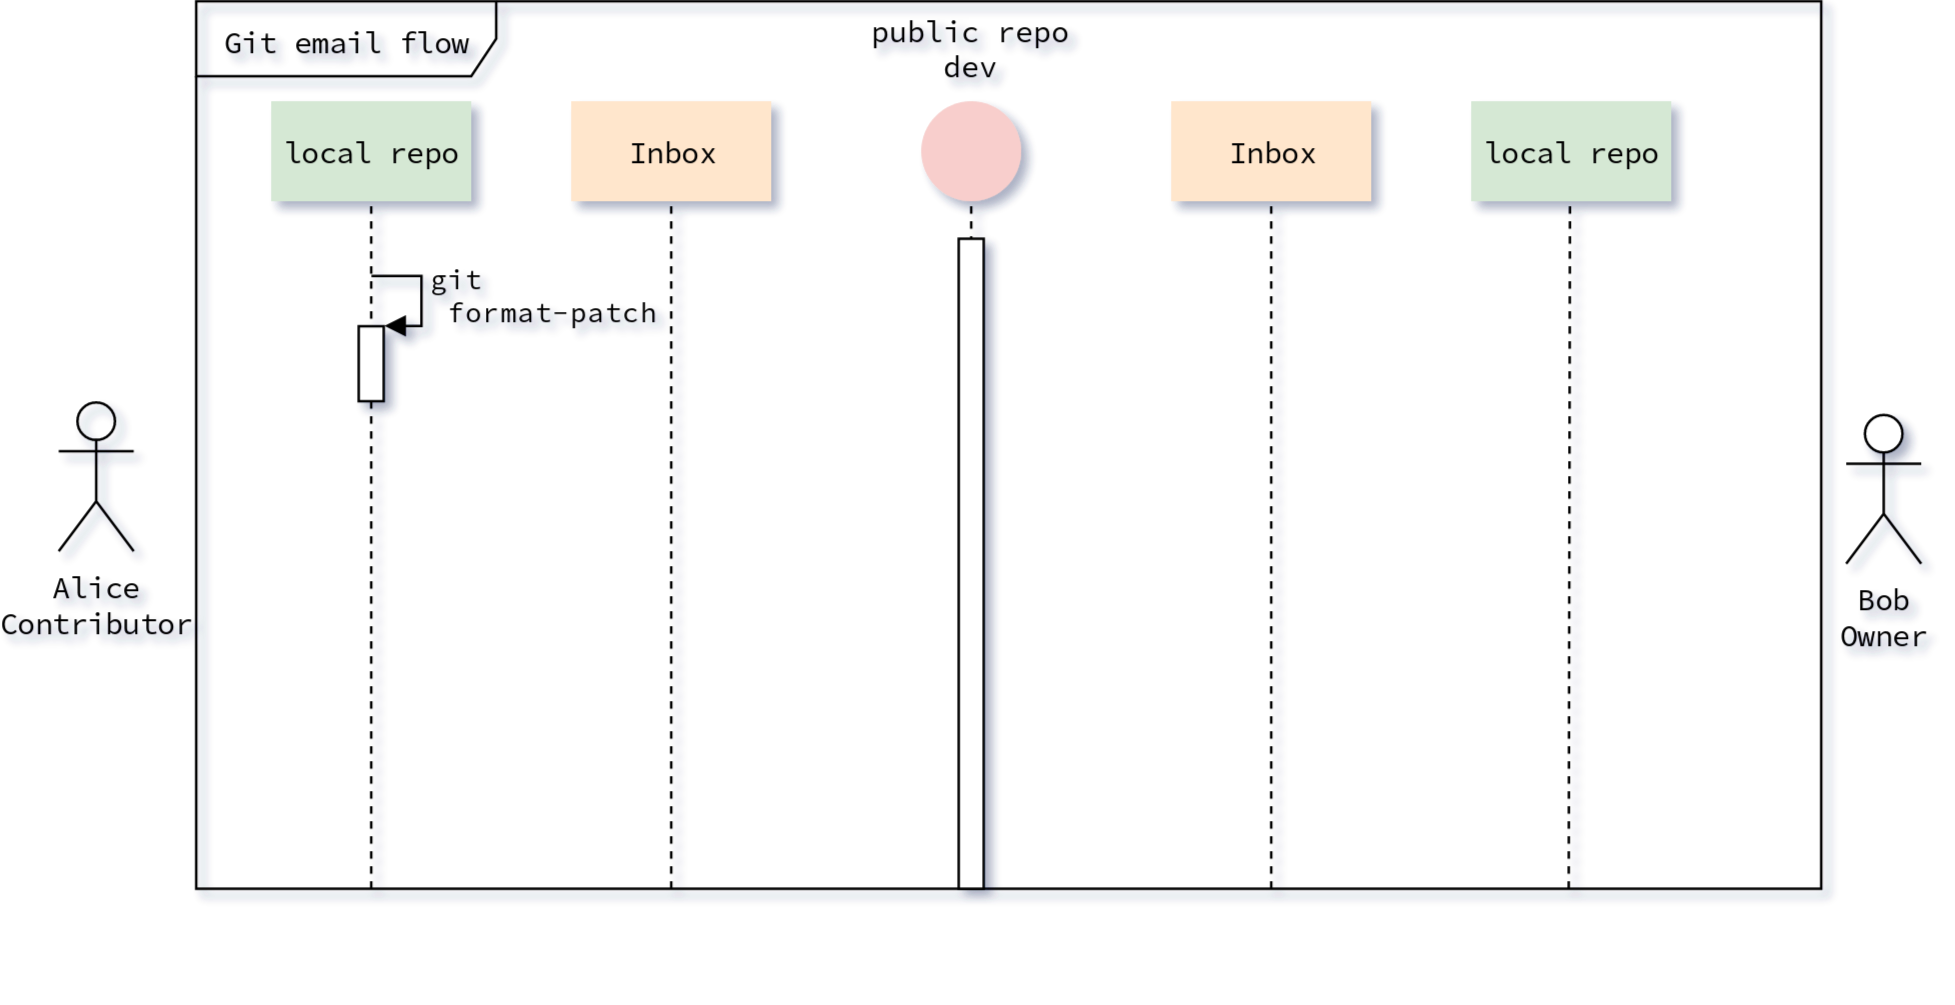
\includegraphics[height=0.75\textheight,keepaspectratio]{./images/EmailWorkflow_PrepareFirstPatch.png}
            }
            \caption{Email workflow}
        \end{center}
    \end{figure}
\end{frame}

\begin{frame}
    \frametitle{Git email}
    \begin{figure}
        \begin{center}
            \ifnumequal{\aspectratio}{43}
            {
                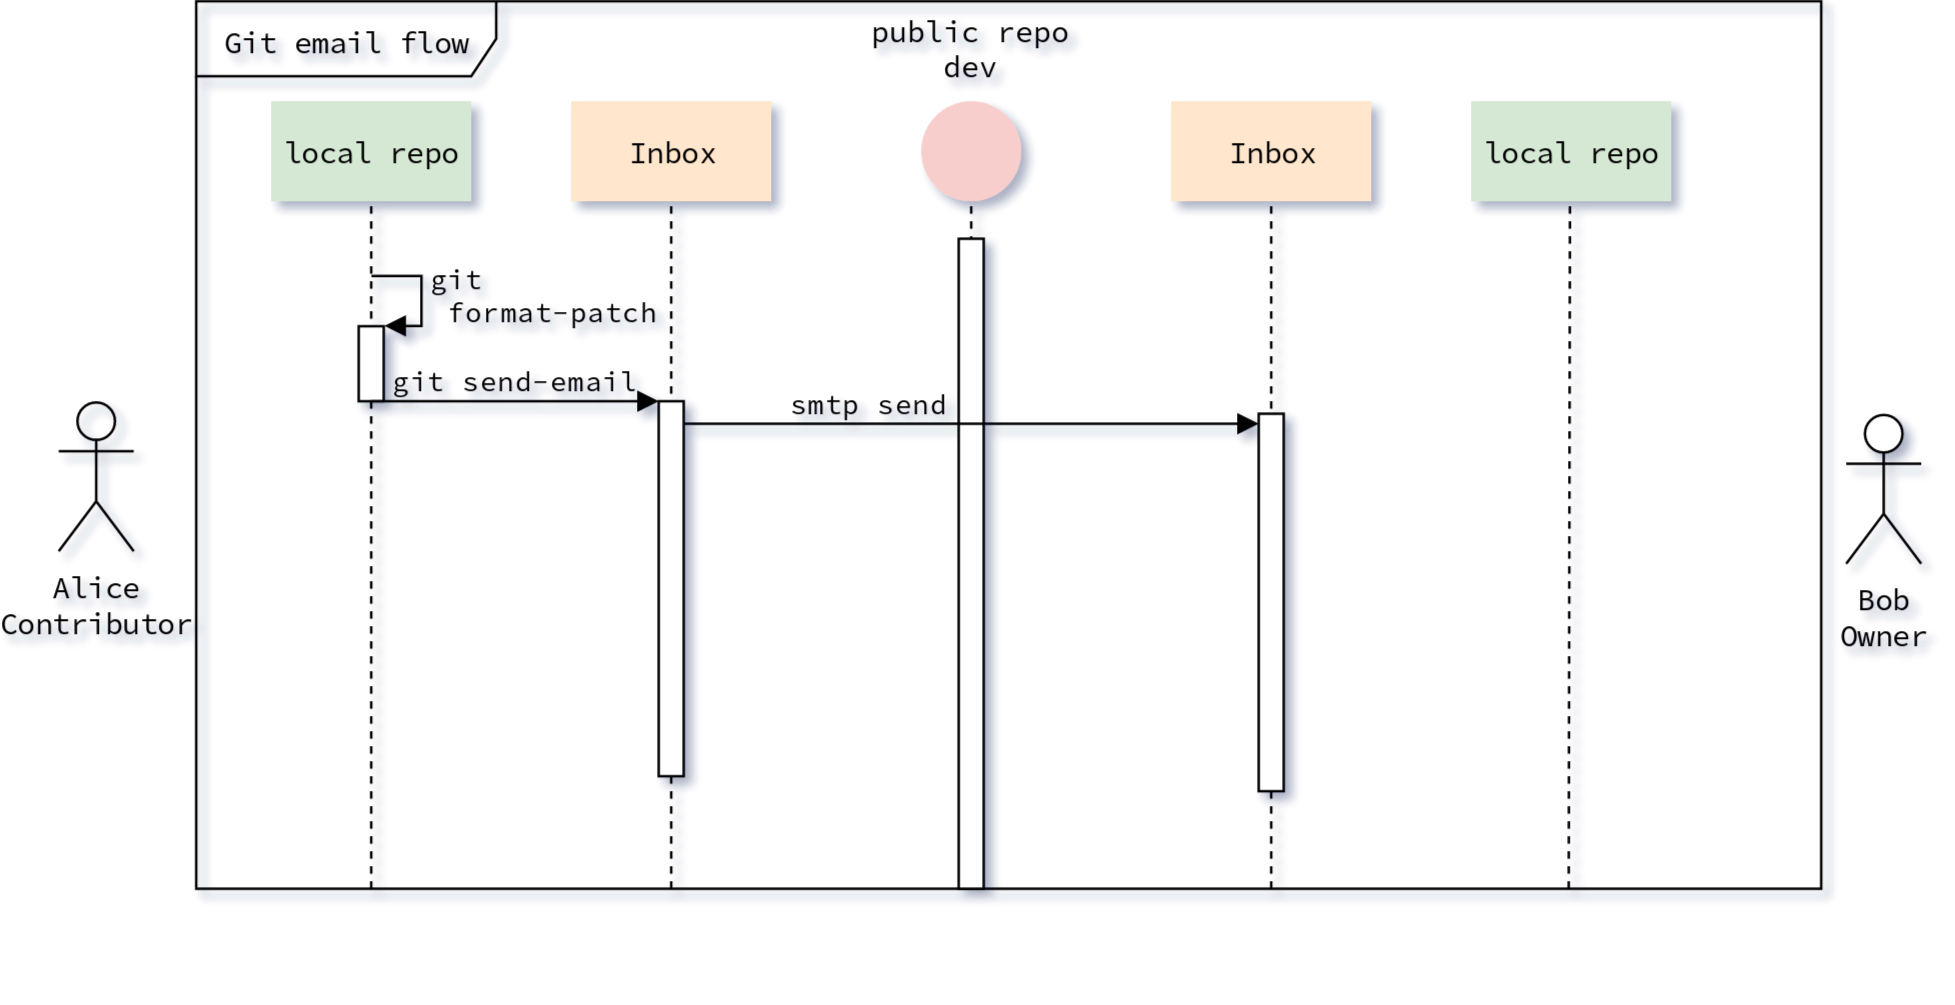
\includegraphics[height=0.7\textheight,keepaspectratio]{./images/EmailWorkflow_SendFirstPatch.png}
            }
            {
                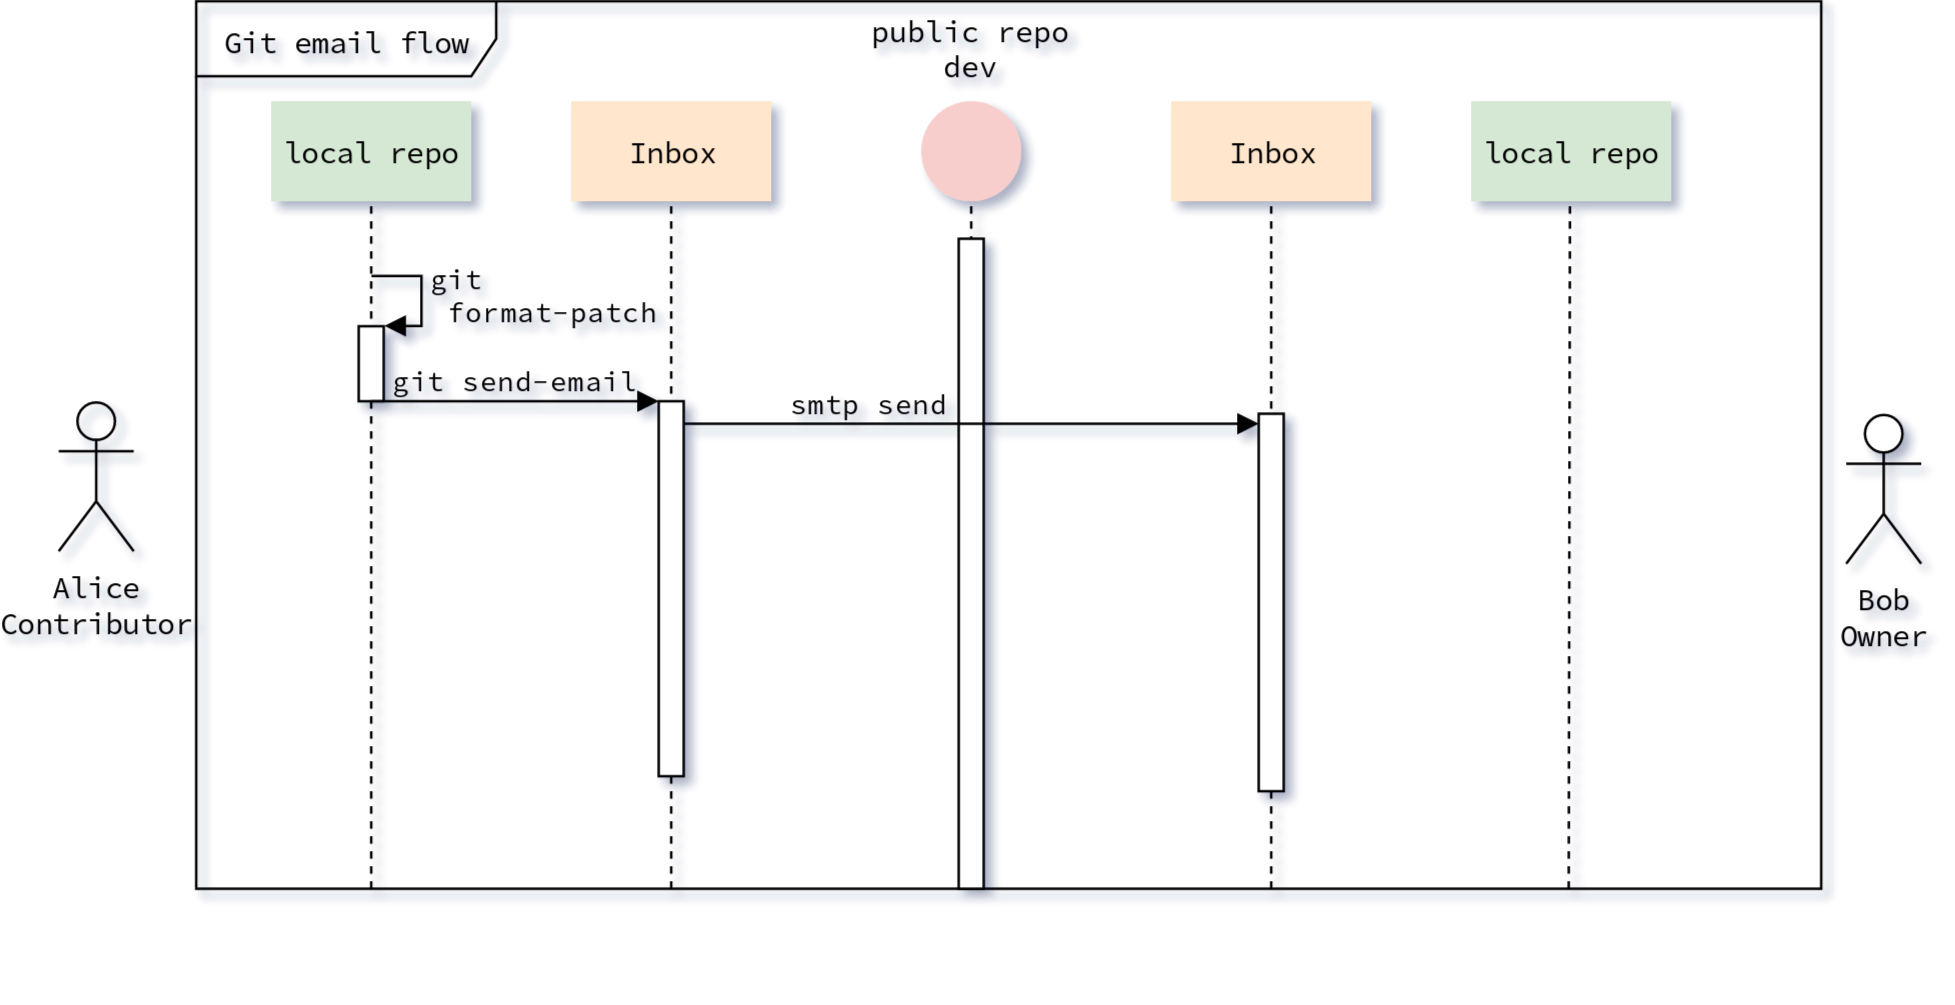
\includegraphics[height=0.75\textheight,keepaspectratio]{./images/EmailWorkflow_SendFirstPatch.png}
            }
            \caption{Email workflow}
        \end{center}
    \end{figure}
\end{frame}

\begin{frame}
    \frametitle{Git email}
    \begin{figure}
        \begin{center}
            \ifnumequal{\aspectratio}{43}
            {
                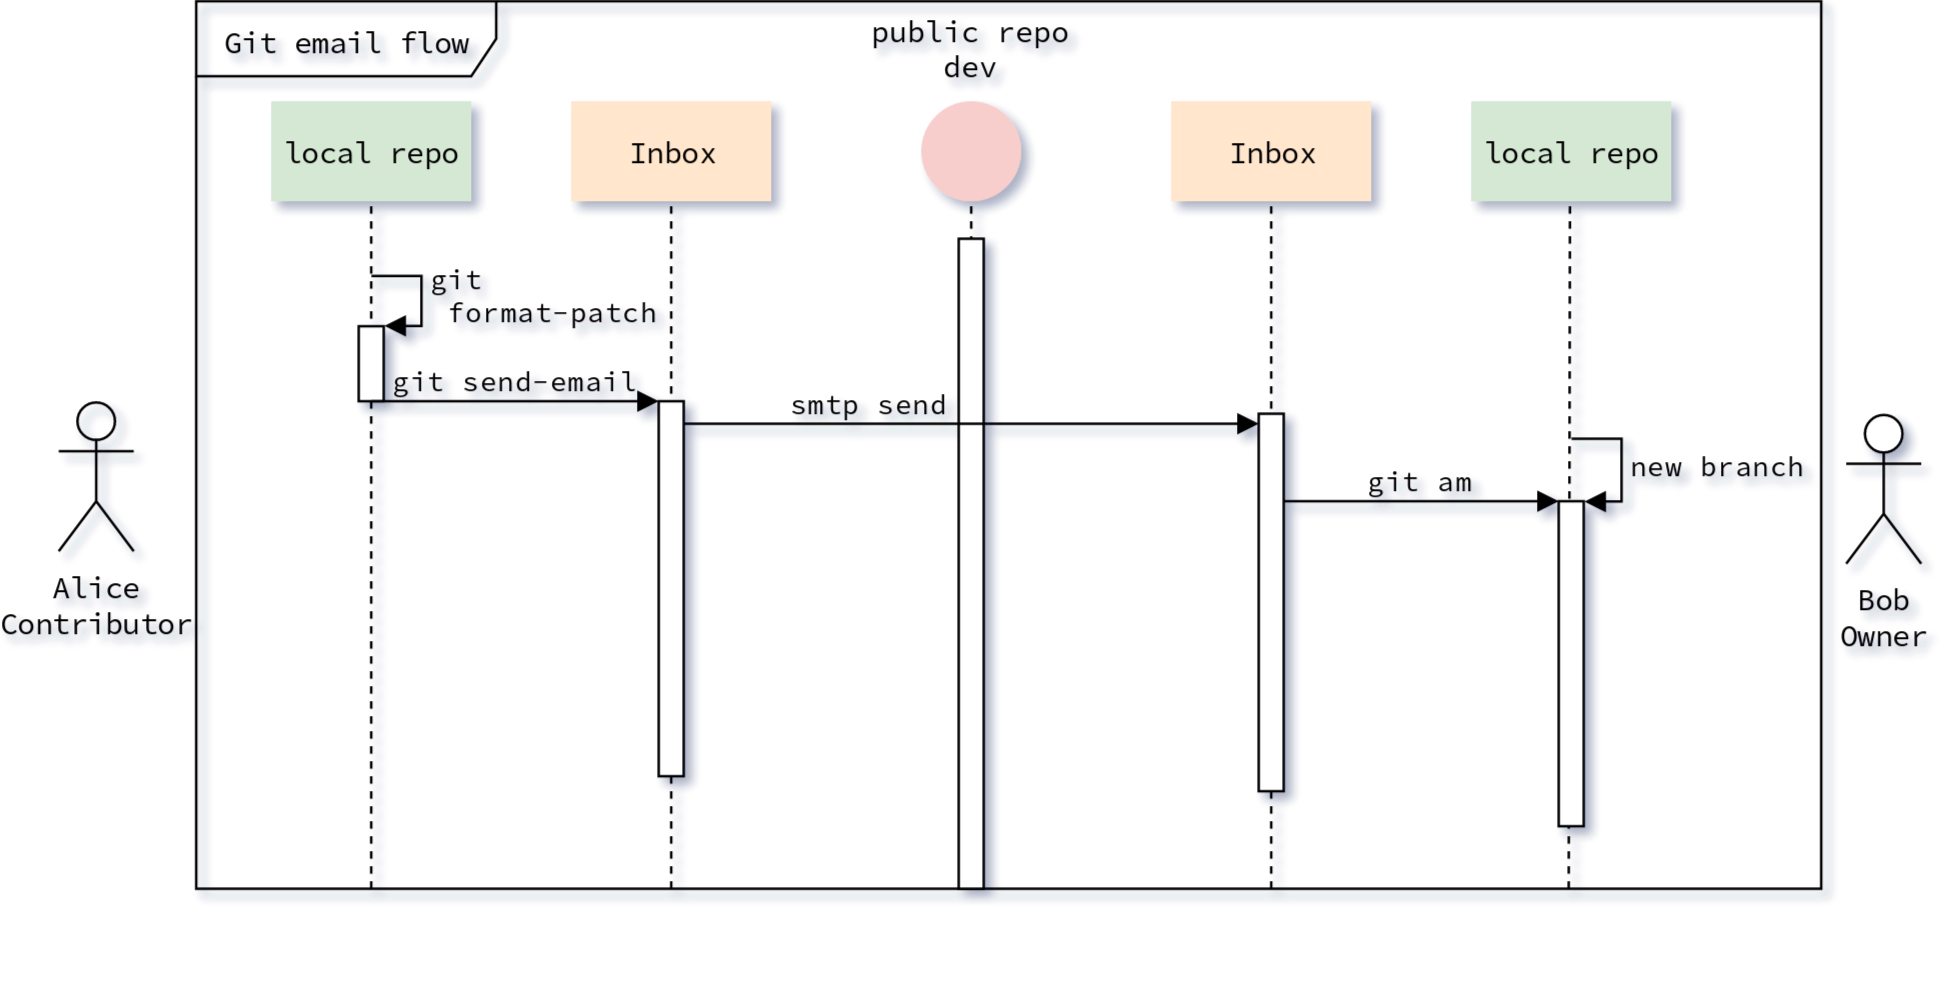
\includegraphics[height=0.7\textheight,keepaspectratio]{./images/EmailWorkflow_ApplyAndTest.png}
            }
            {
                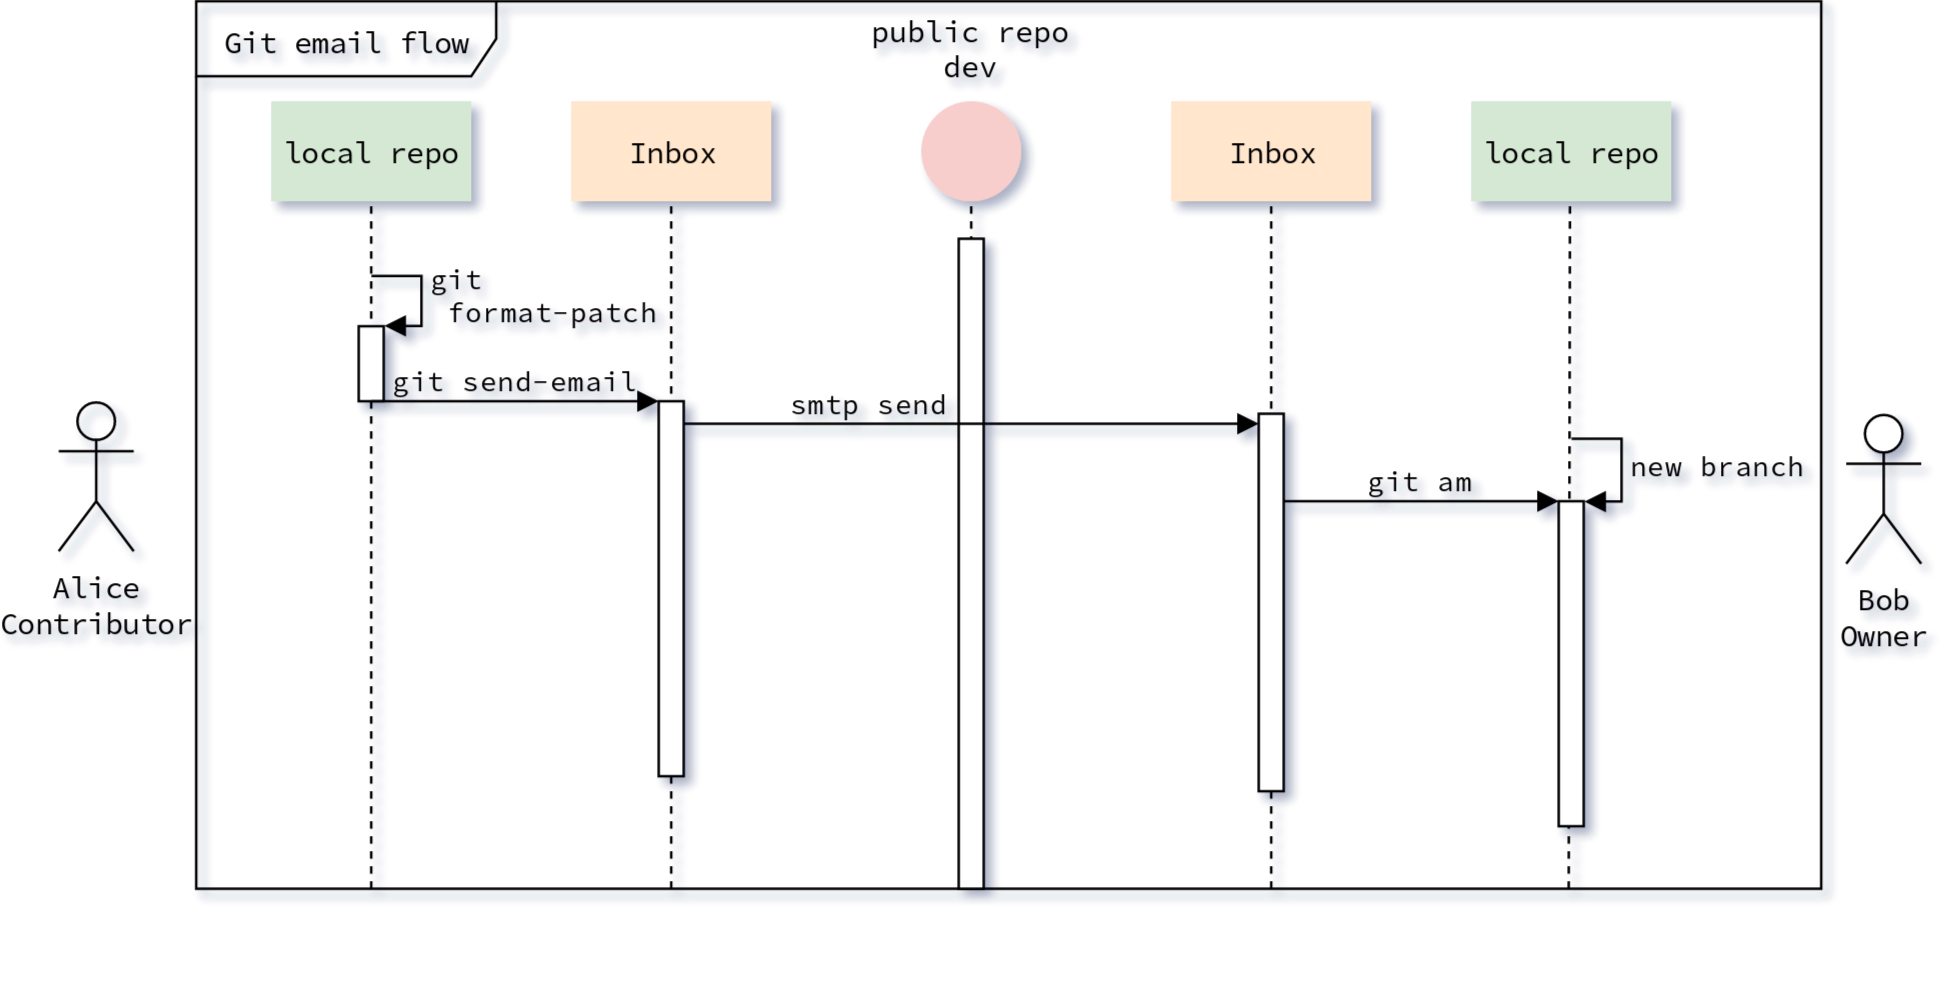
\includegraphics[height=0.75\textheight,keepaspectratio]{./images/EmailWorkflow_ApplyAndTest.png}
            }
            \caption{Email workflow}
        \end{center}
    \end{figure}
\end{frame}

\begin{frame}
    \frametitle{Git email}
    \begin{figure}
        \begin{center}
            \ifnumequal{\aspectratio}{43}
            {
                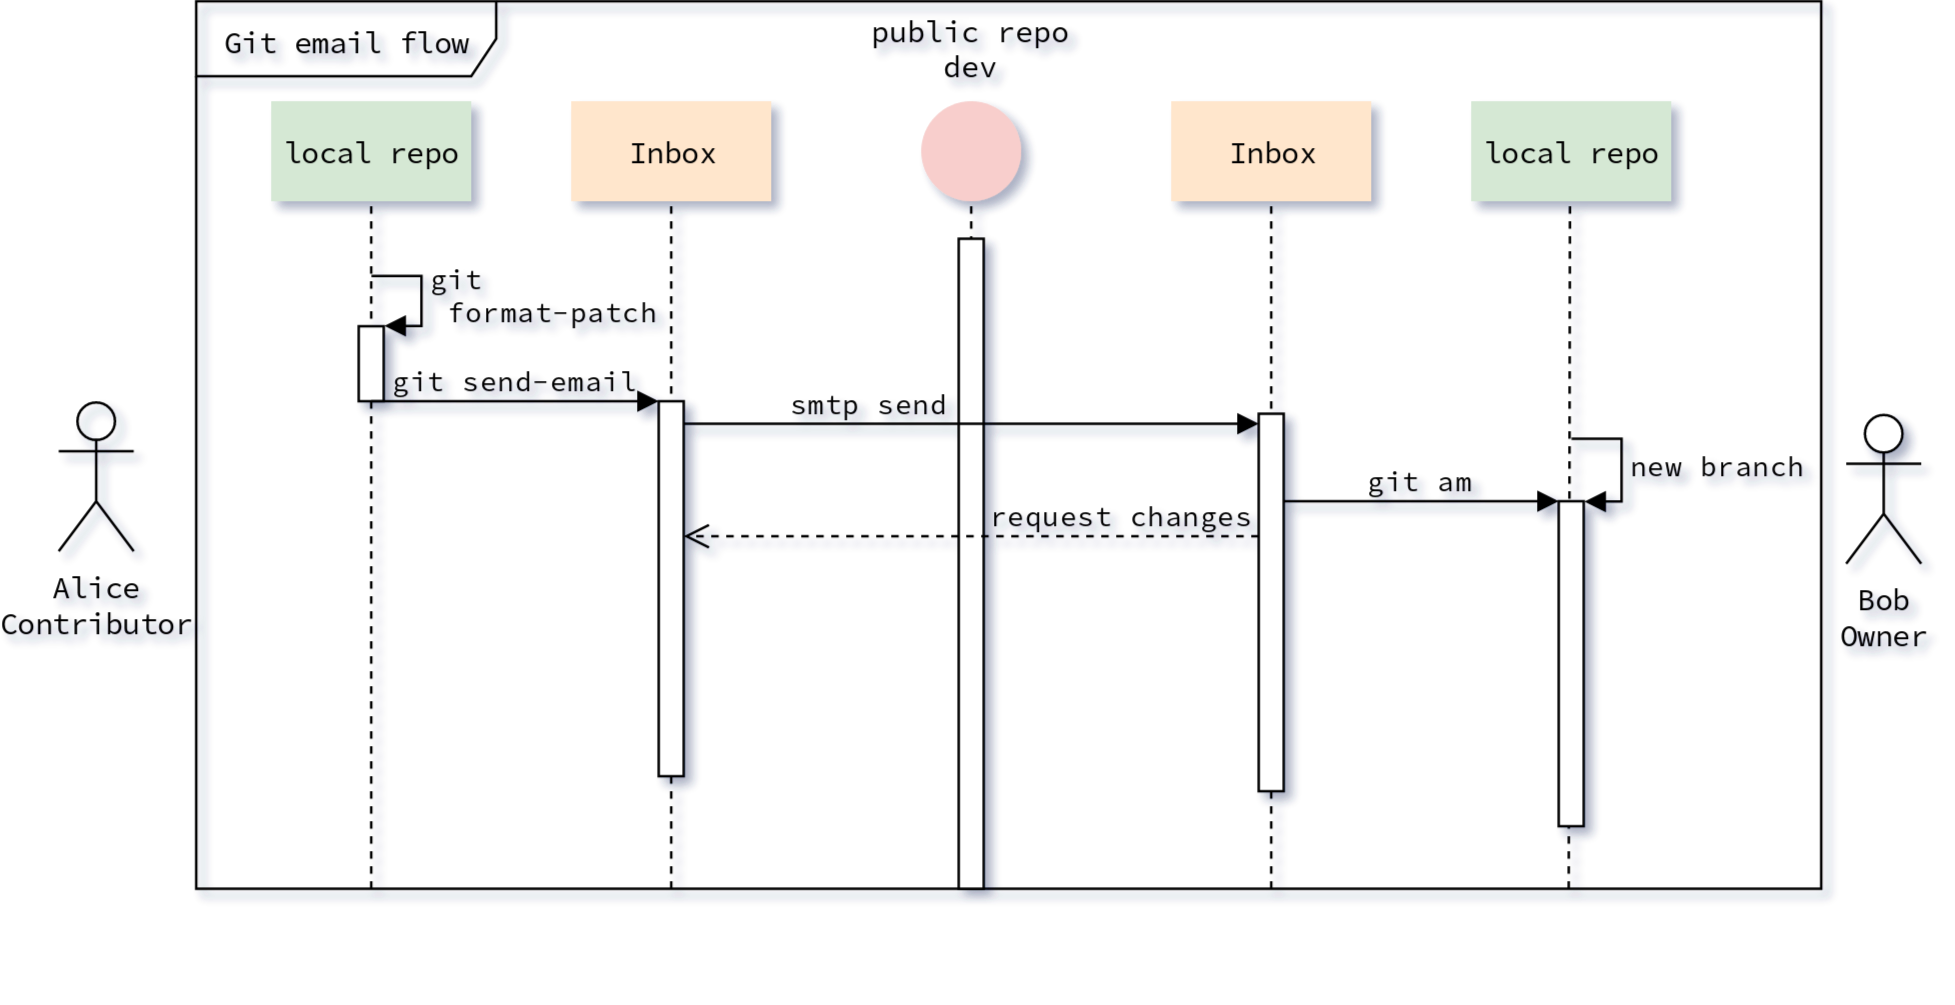
\includegraphics[height=0.7\textheight,keepaspectratio]{./images/EmailWorkflow_RequestChanges.png}
            }
            {
                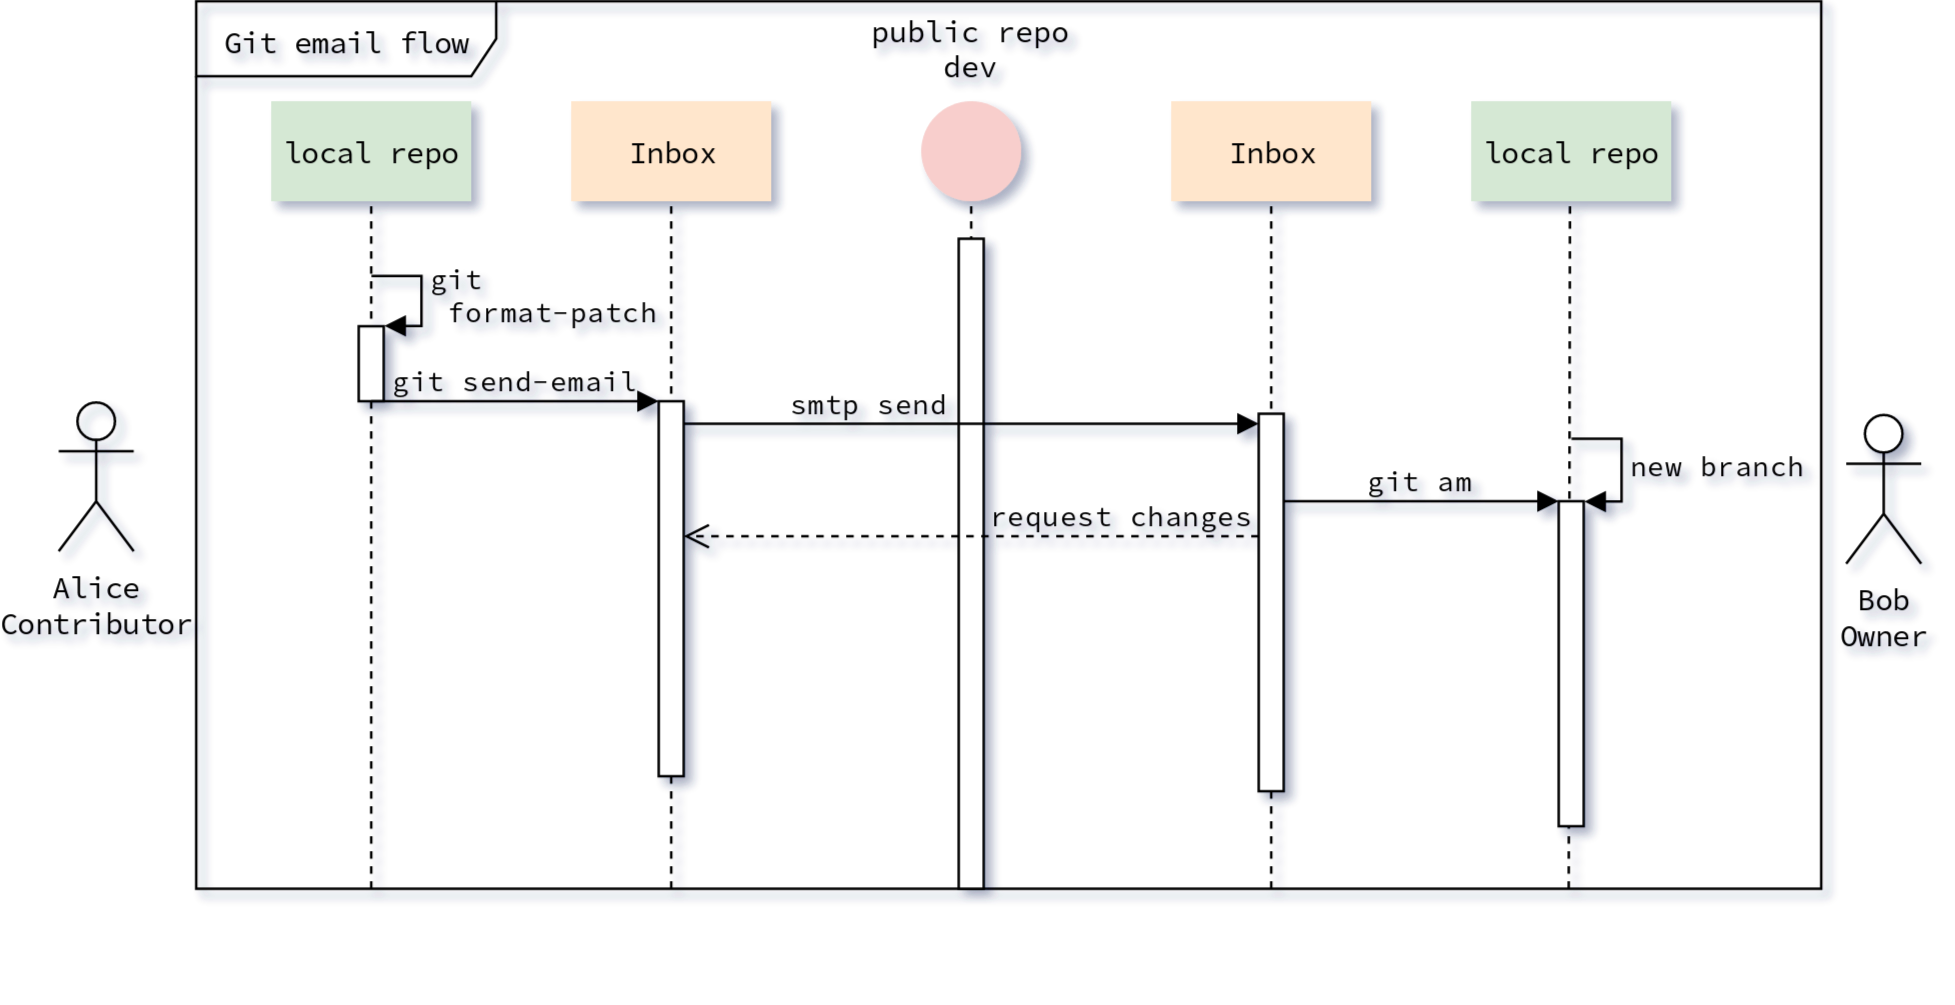
\includegraphics[height=0.75\textheight,keepaspectratio]{./images/EmailWorkflow_RequestChanges.png}
            }
            \caption{Email workflow}
        \end{center}
    \end{figure}
\end{frame}

\begin{frame}
    \frametitle{Git email}
    \begin{figure}
        \begin{center}
            \ifnumequal{\aspectratio}{43}
            {
                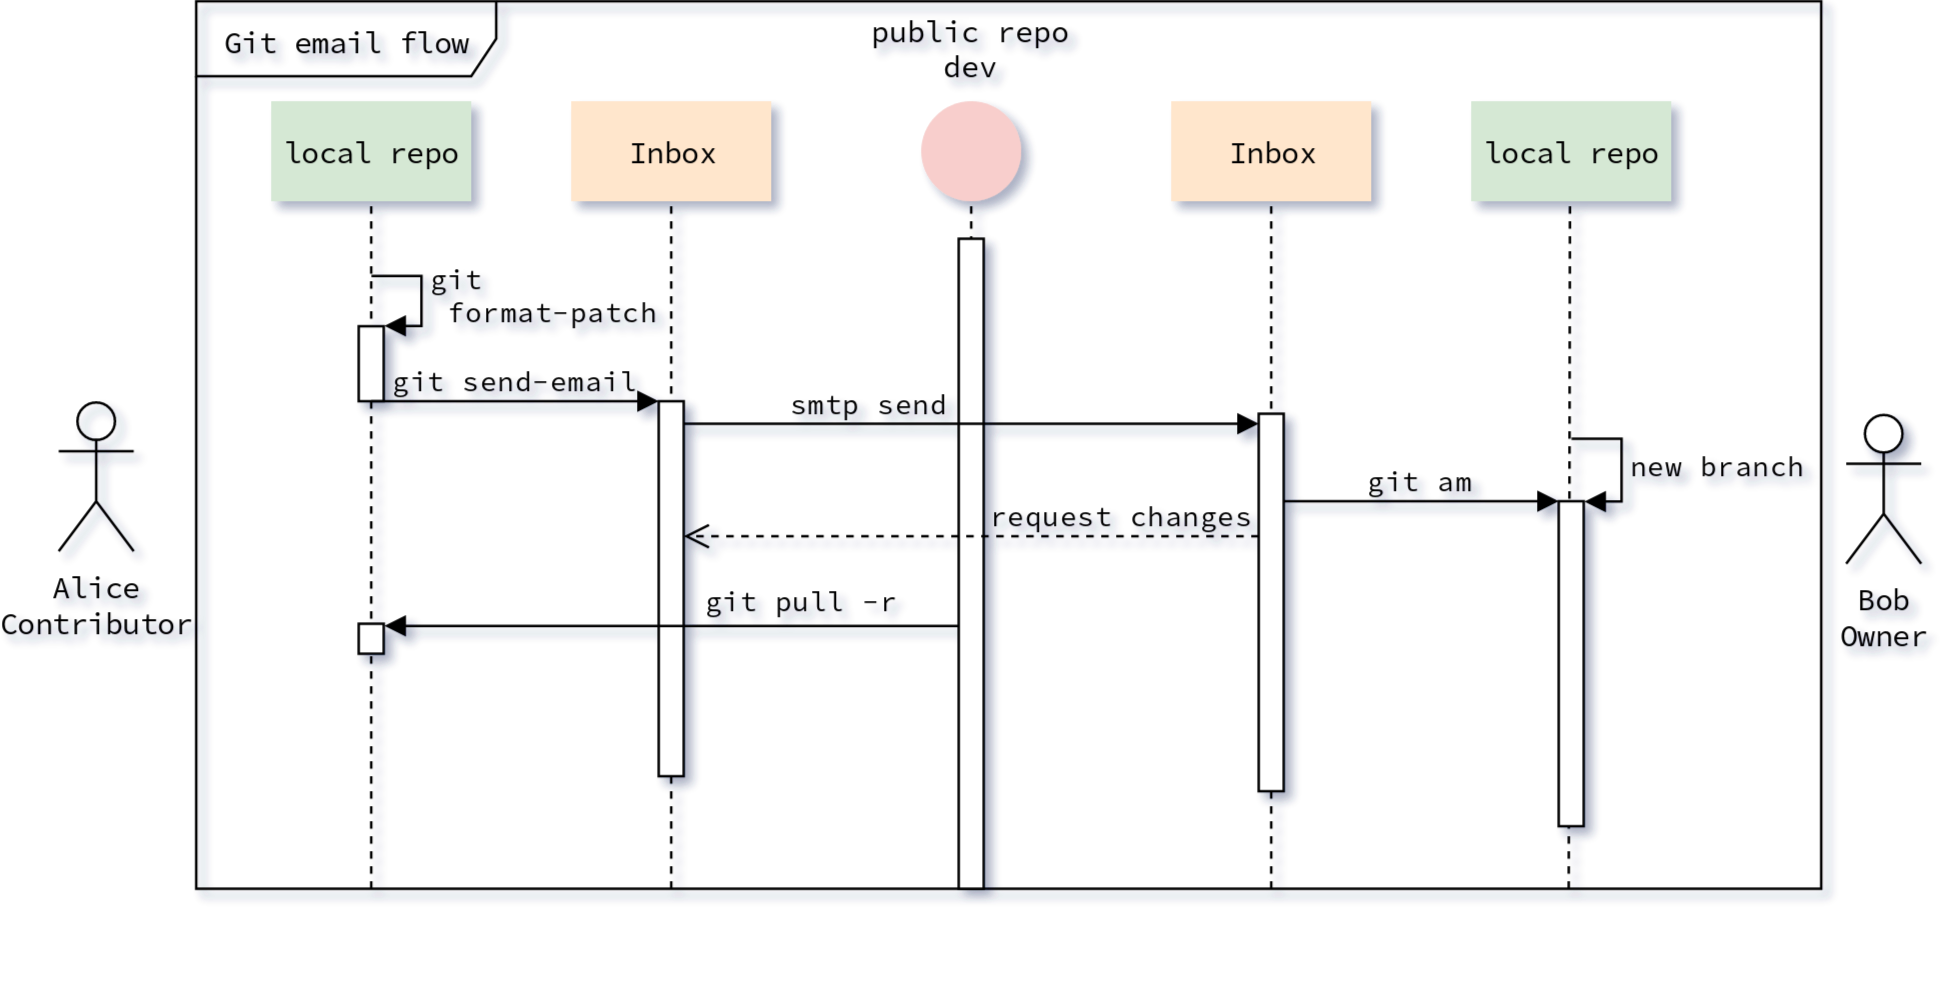
\includegraphics[height=0.7\textheight,keepaspectratio]{./images/EmailWorkflow_UpdateLocalRepository.png}
            }
            {
                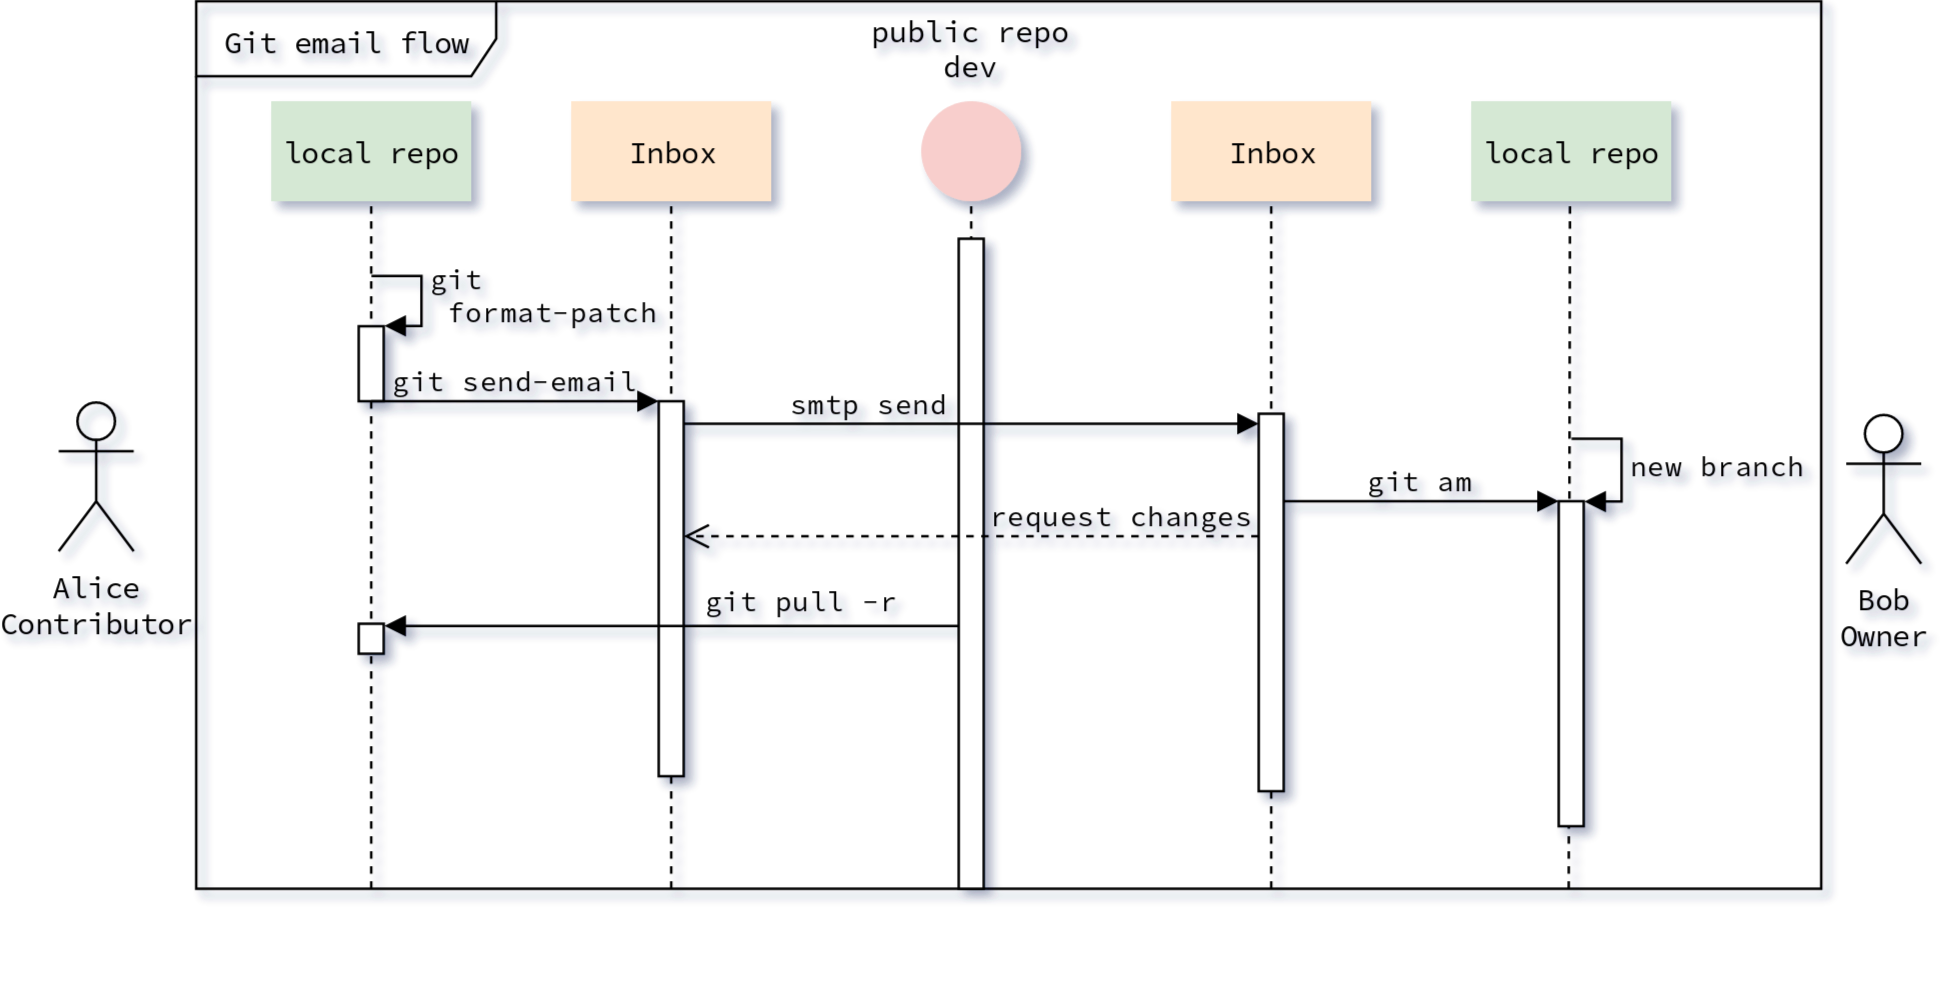
\includegraphics[height=0.75\textheight,keepaspectratio]{./images/EmailWorkflow_UpdateLocalRepository.png}
            }
            \caption{Email workflow}
        \end{center}
    \end{figure}
\end{frame}

\begin{frame}
    \frametitle{Git email}
    \begin{figure}
        \begin{center}
            \ifnumequal{\aspectratio}{43}
            {
                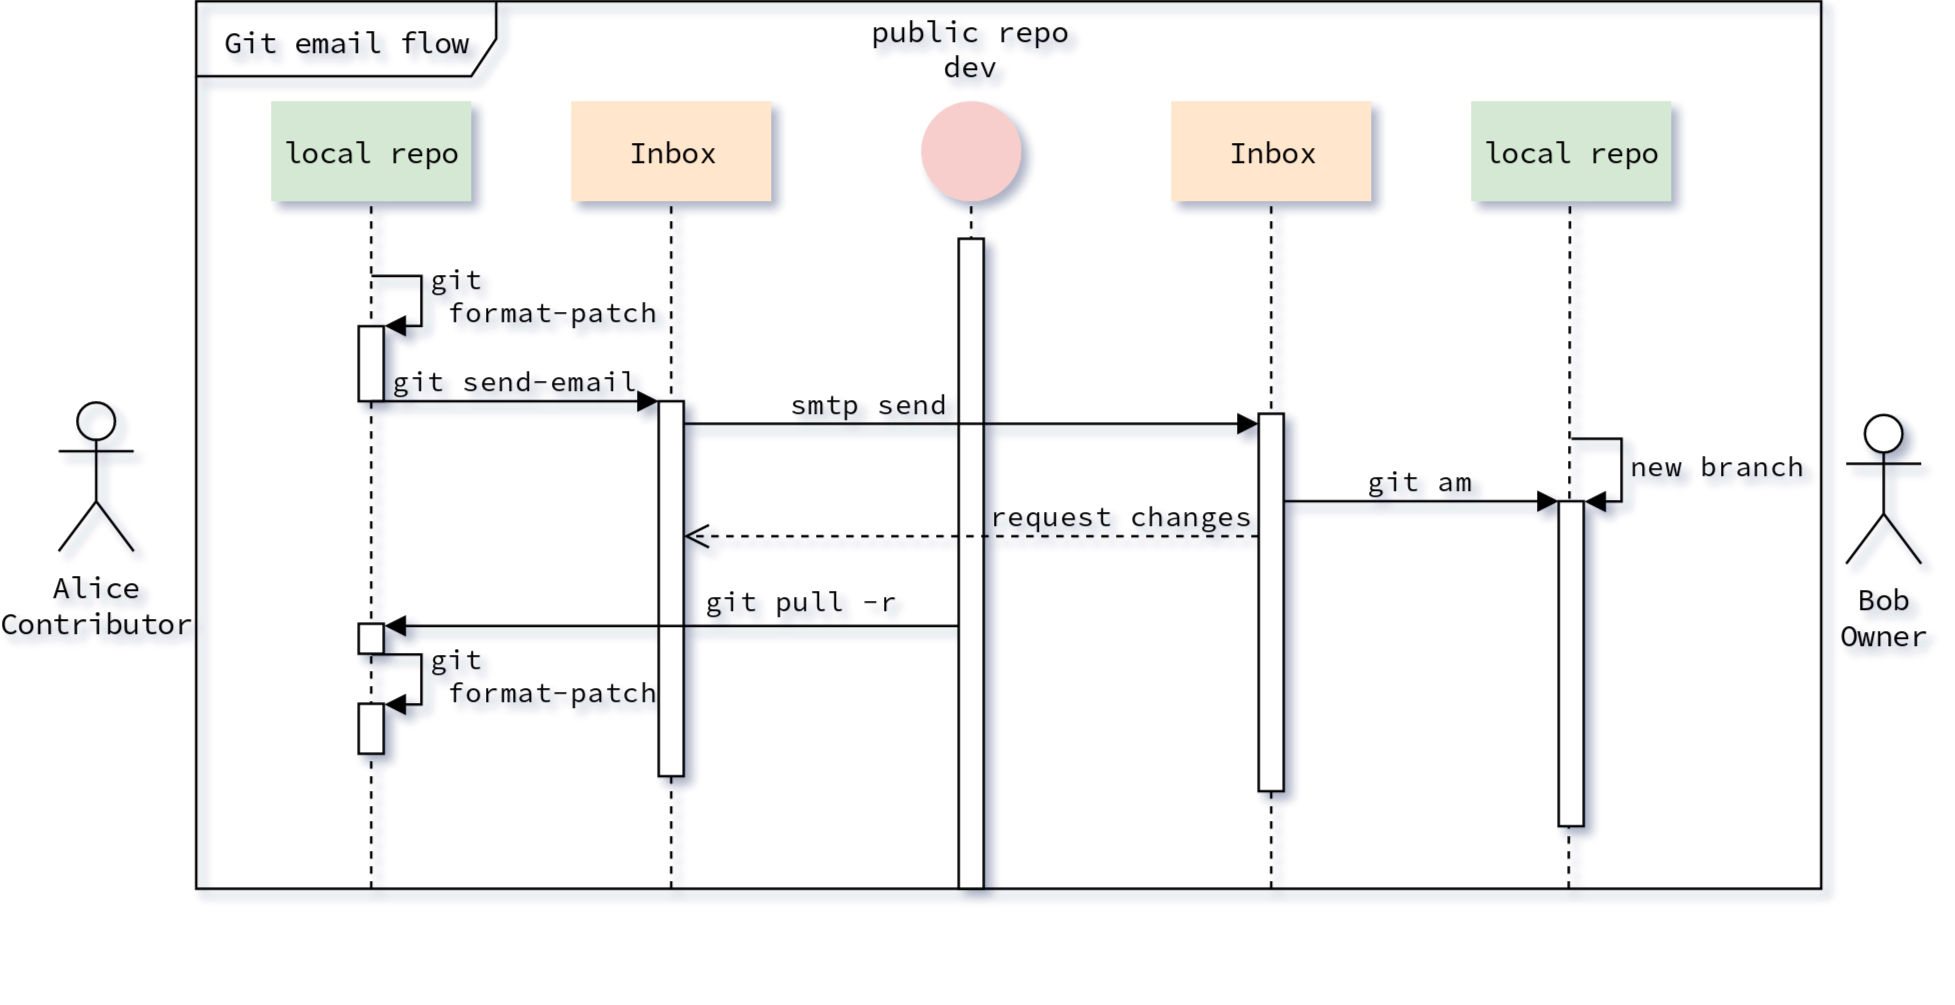
\includegraphics[height=0.7\textheight,keepaspectratio]{./images/EmailWorkflow_PrepareSecoundPatch.png}
            }
            {
                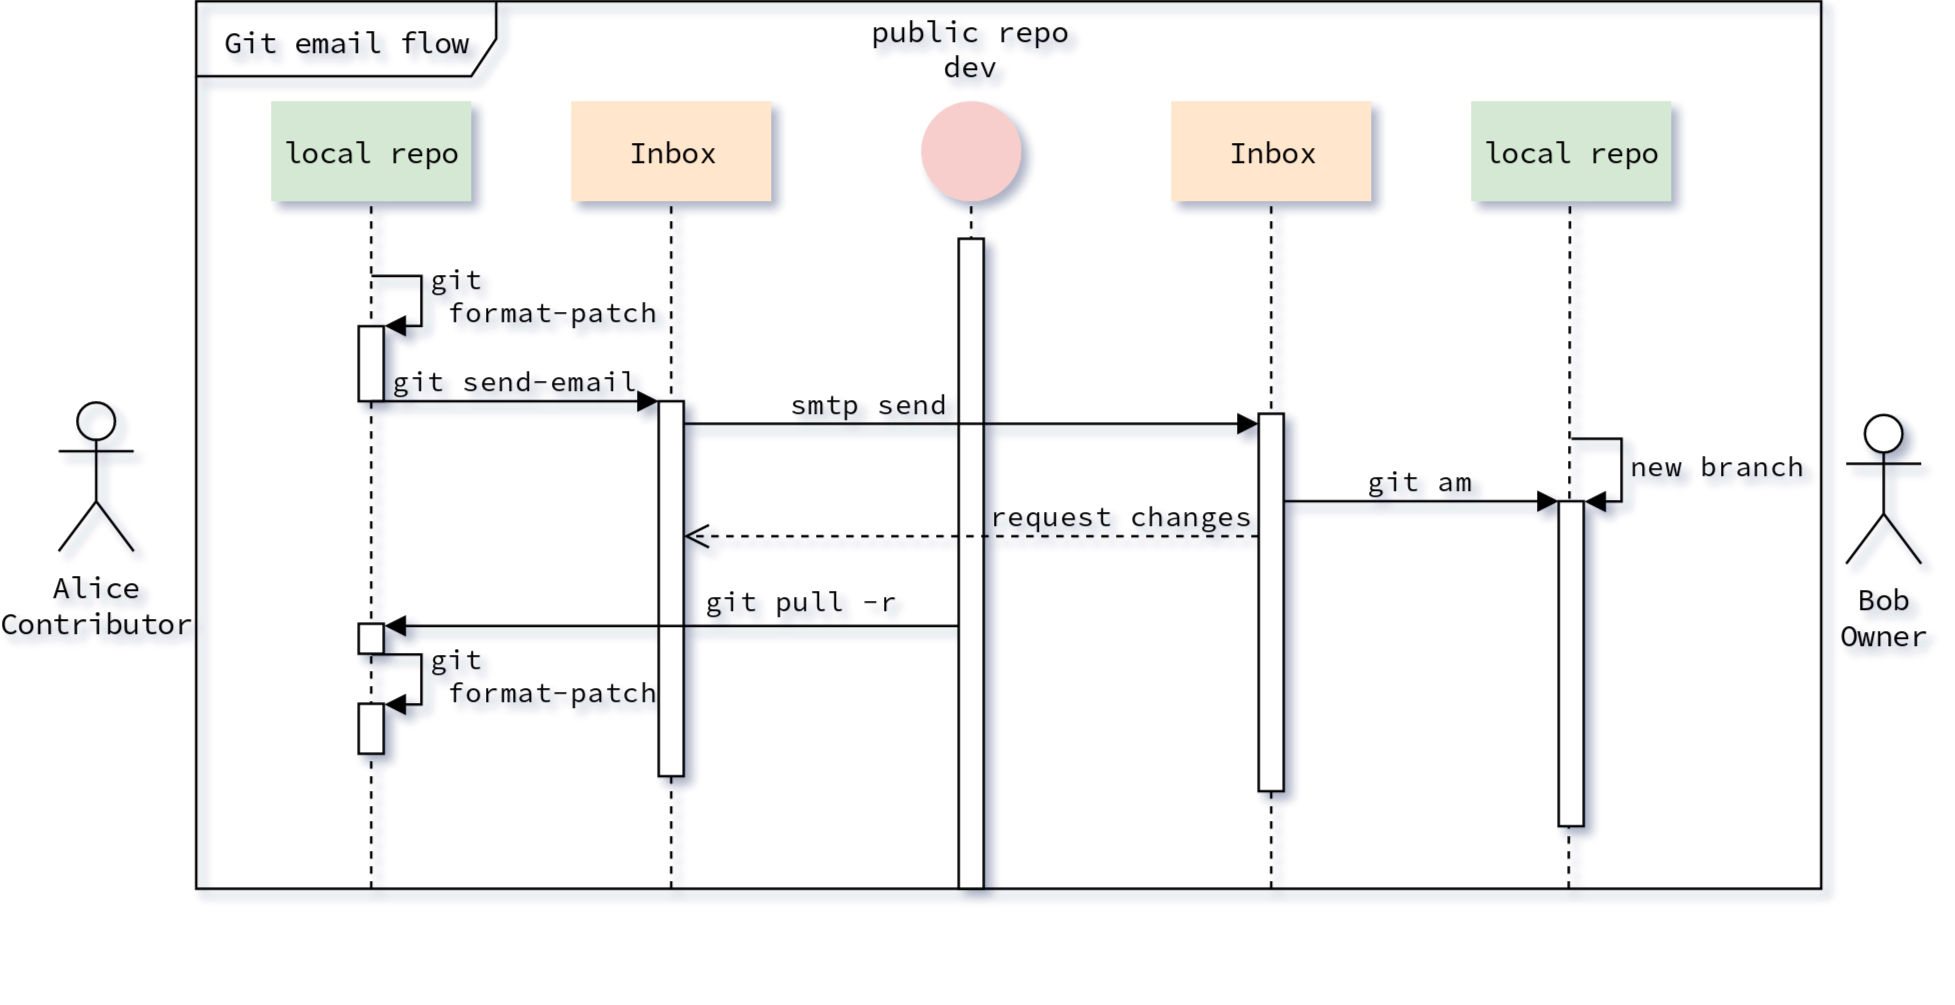
\includegraphics[height=0.75\textheight,keepaspectratio]{./images/EmailWorkflow_PrepareSecoundPatch.png}
            }
            \caption{Email workflow}
        \end{center}
    \end{figure}
\end{frame}

\begin{frame}
    \frametitle{Git email}
    \begin{figure}
        \begin{center}
            \ifnumequal{\aspectratio}{43}
            {
                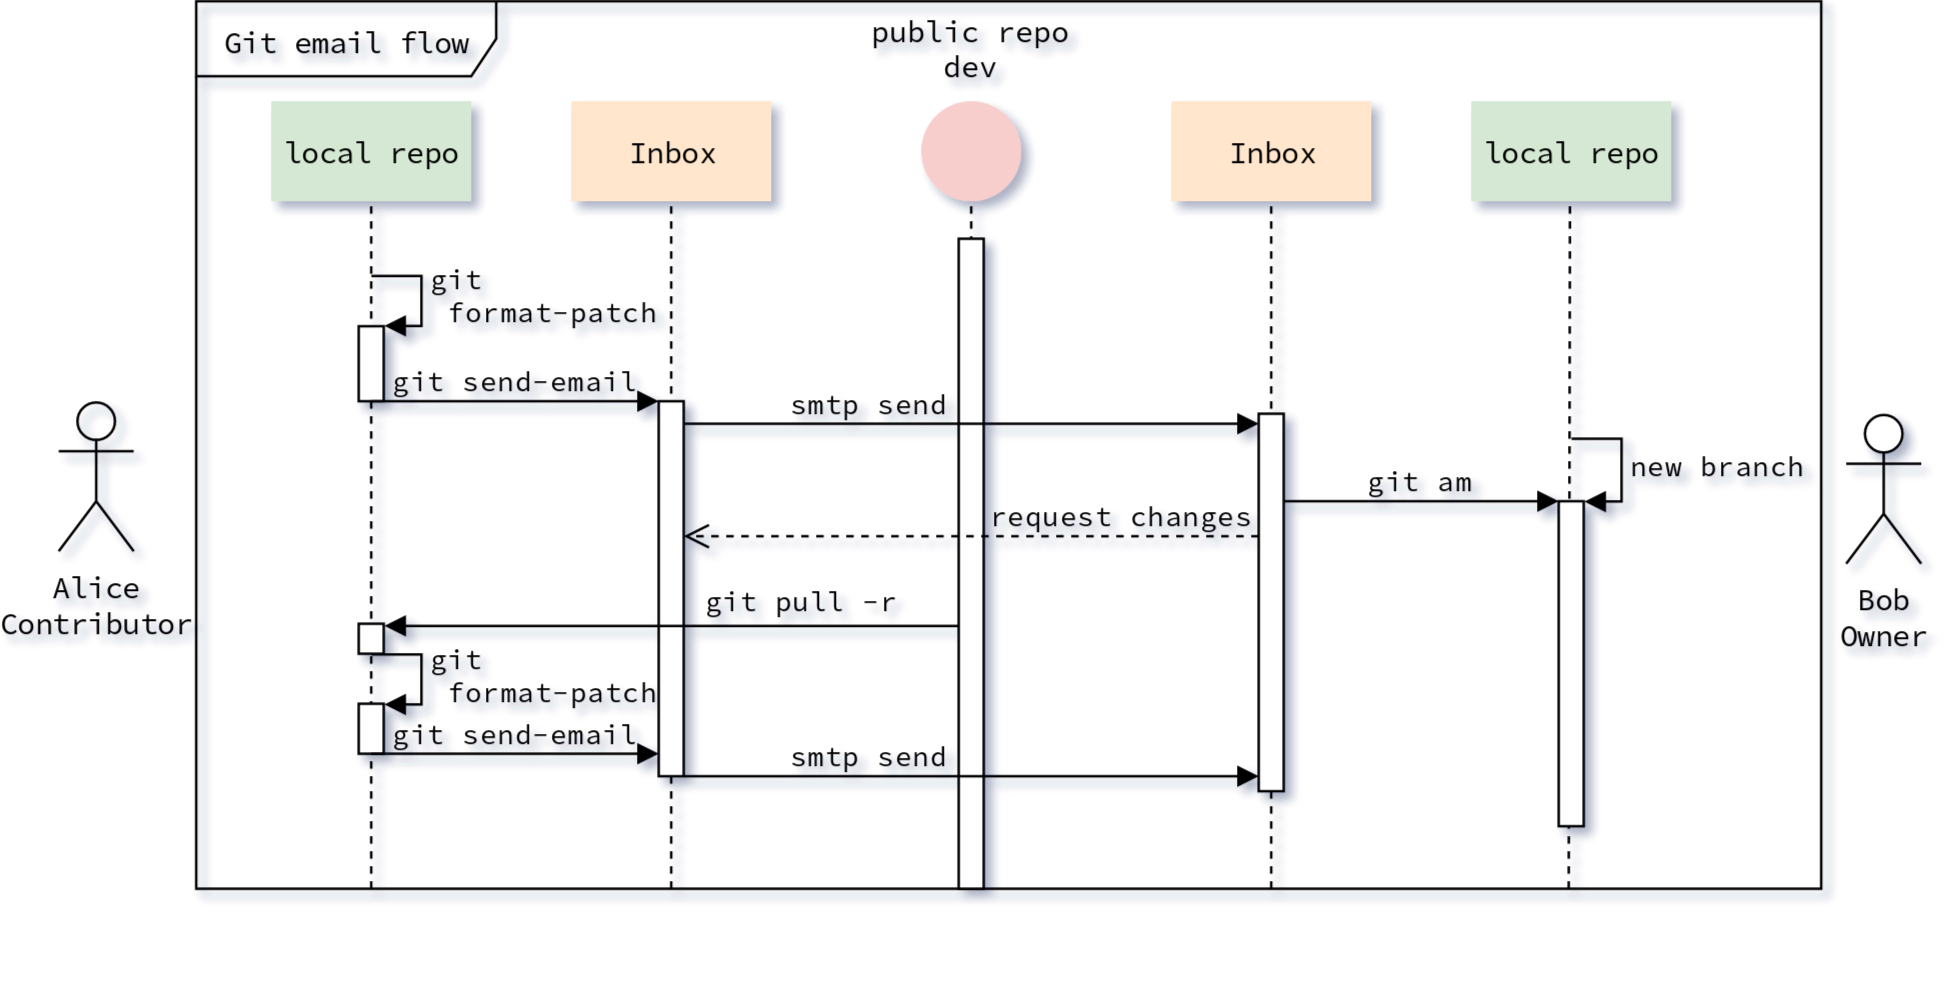
\includegraphics[height=0.7\textheight,keepaspectratio]{./images/EmailWorkflow_SendSecoundPatch.png}
            }
            {
                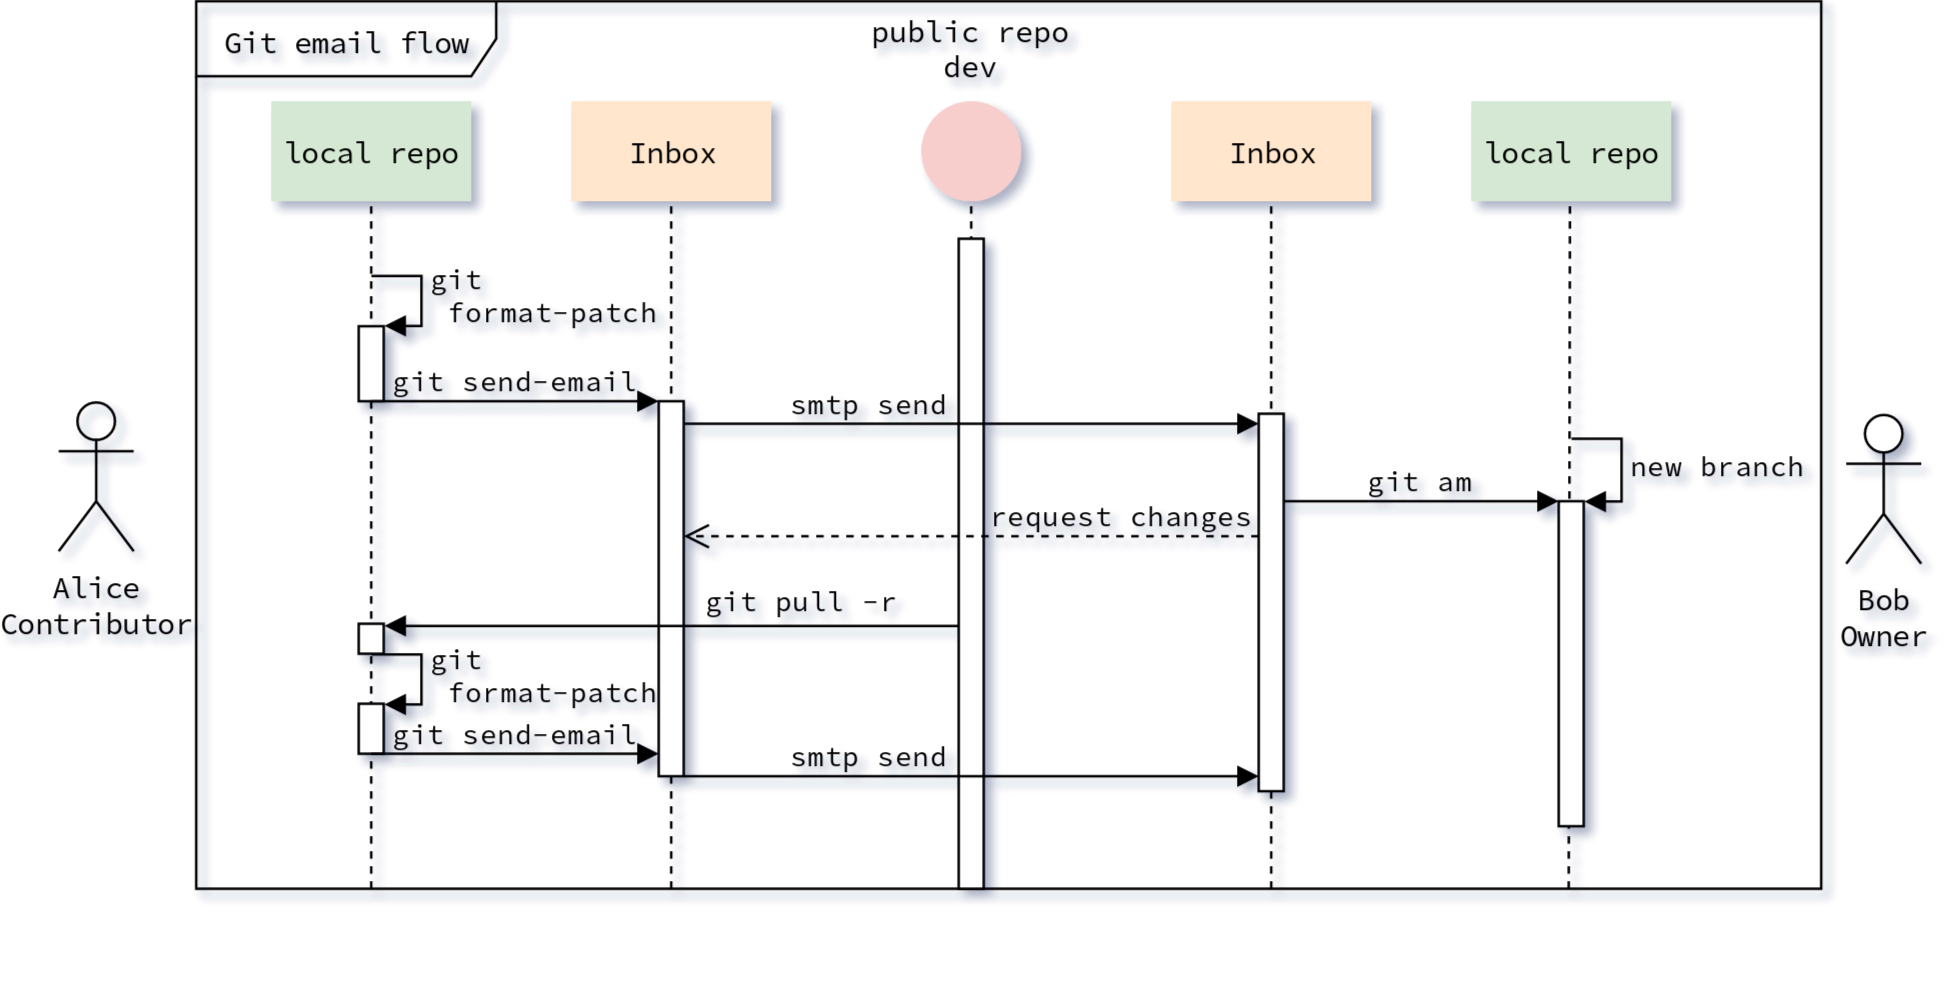
\includegraphics[height=0.75\textheight,keepaspectratio]{./images/EmailWorkflow_SendSecoundPatch.png}
            }
            \caption{Email workflow}
        \end{center}
    \end{figure}
\end{frame}

\begin{frame}
    \frametitle{Git email}
    \begin{figure}
        \begin{center}
            \ifnumequal{\aspectratio}{43}
            {
                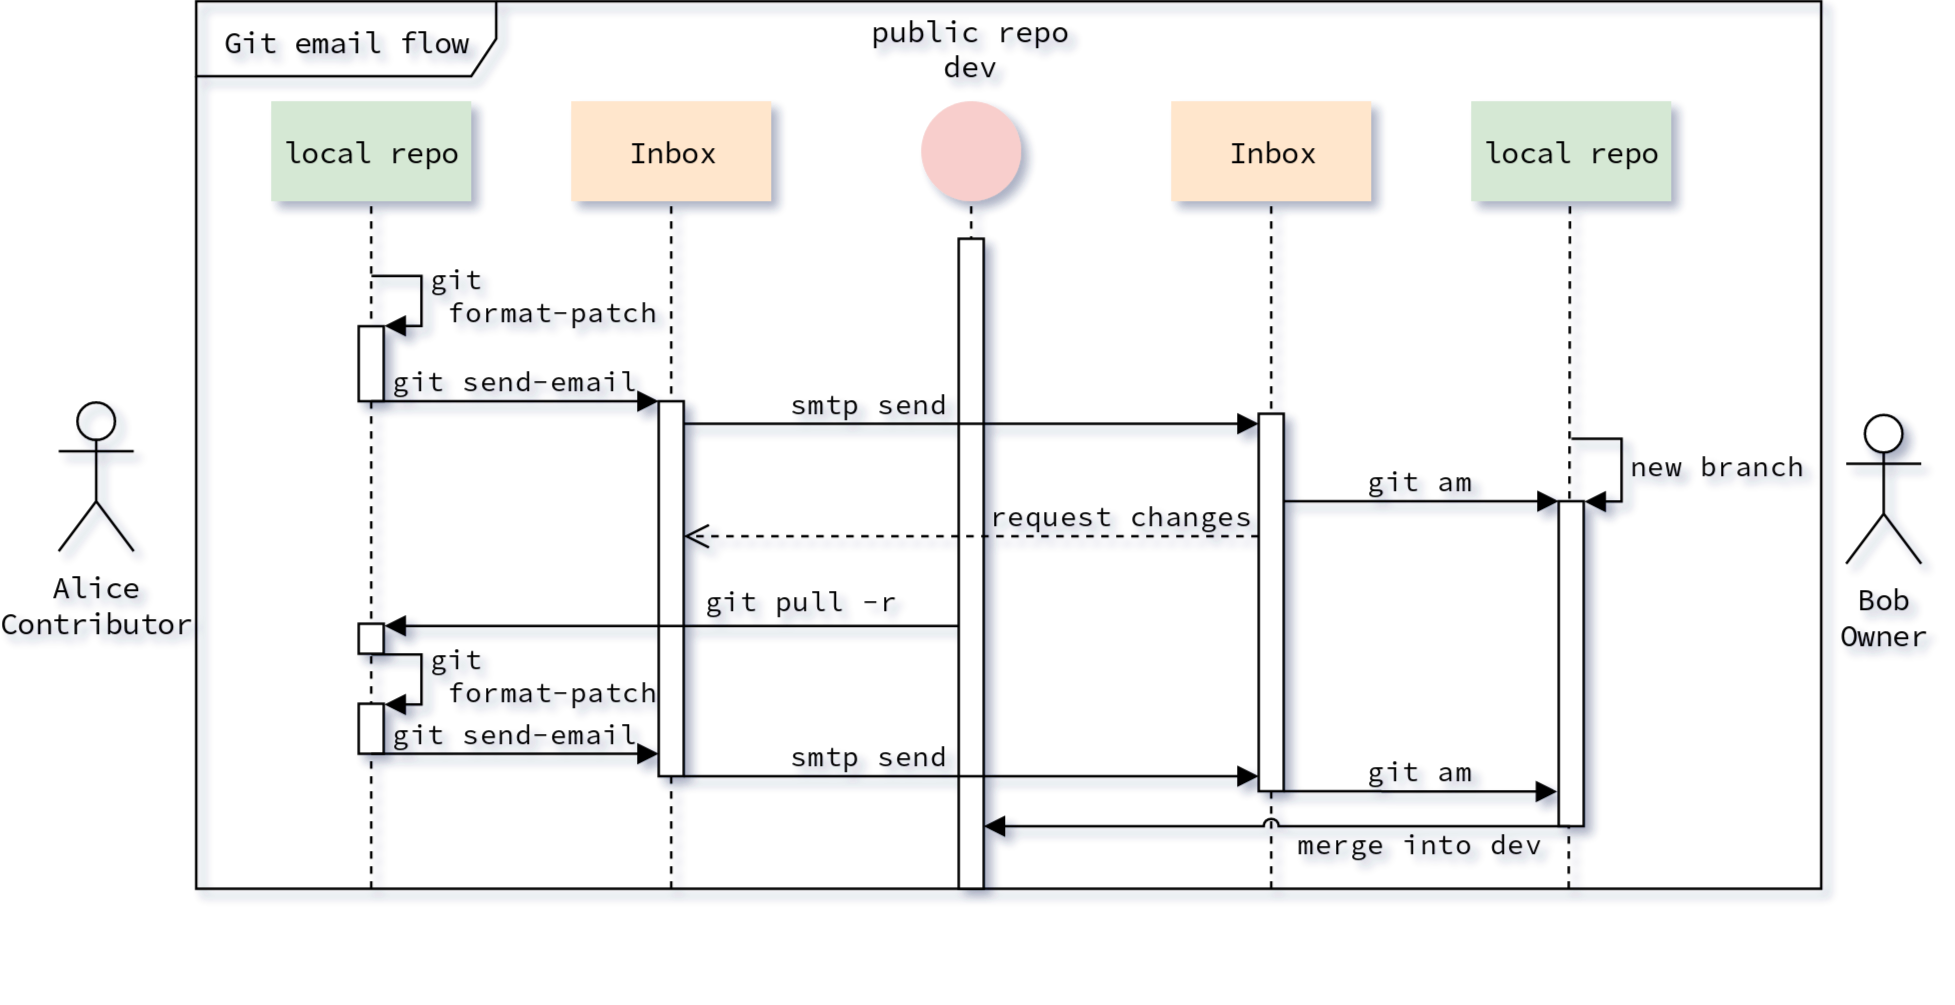
\includegraphics[height=0.7\textheight,keepaspectratio]{./images/EmailWorkflow_ApplyAndMerge.png}
            }
            {
                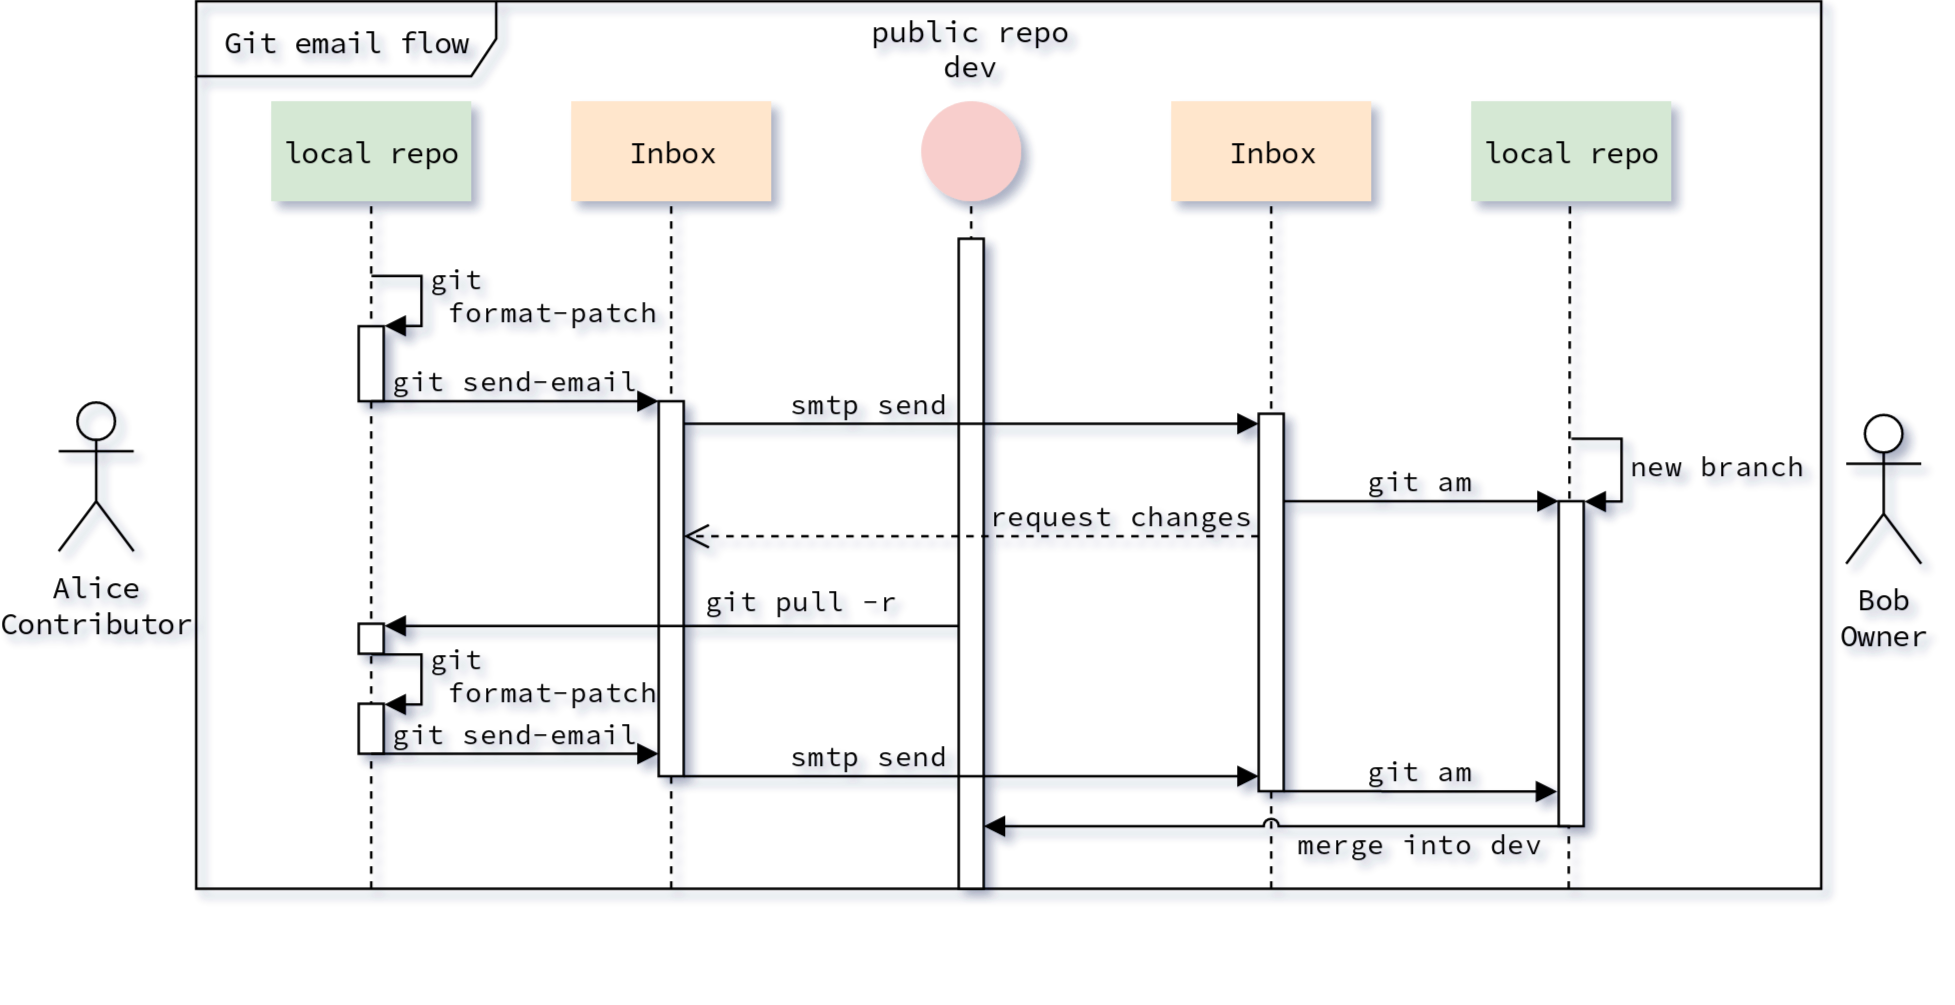
\includegraphics[height=0.75\textheight,keepaspectratio]{./images/EmailWorkflow_ApplyAndMerge.png}
            }
            \caption{Email workflow}
        \end{center}
    \end{figure}
\end{frame}



    \subsection{Recap}
\begin{frame}
    \frametitle{Recap email}
    \begin{itemize}
        \item Development stays the same
        \item The integrator
        \item Offline availability with stored emails
    \end{itemize}
\end{frame}



    \section{Cherry picking}
\begin{frame}
    \frametitle{When to use cherry-pick}
    \begin{itemize}
        \item commit on the wrong branch
        \begin{itemize}
            \item cherry-pick it into the desired branch
            \item reset the orignal branch
        \end{itemize}
        \item you don't want to merge a whole branch
        \item as part of \texttt{git rebase}
    \end{itemize}
\end{frame}

\begin{frame}
    \frametitle{What does cherry-pick do}
    \begin{itemize}
        \item copies the content of the commit
        \item metadata like author and date are kept
    \end{itemize}
    \begin{alertblock}{Be aware of}
        \begin{itemize}
            \item changes the commit sha1
            \item different parents
        \end{itemize}
    \end{alertblock}
\end{frame}

\begin{frame}[fragile]
    \frametitle{What does rebase do}
    \begin{figure}
        \begin{center}
            \ifnumequal{\aspectratio}{43}
            {
                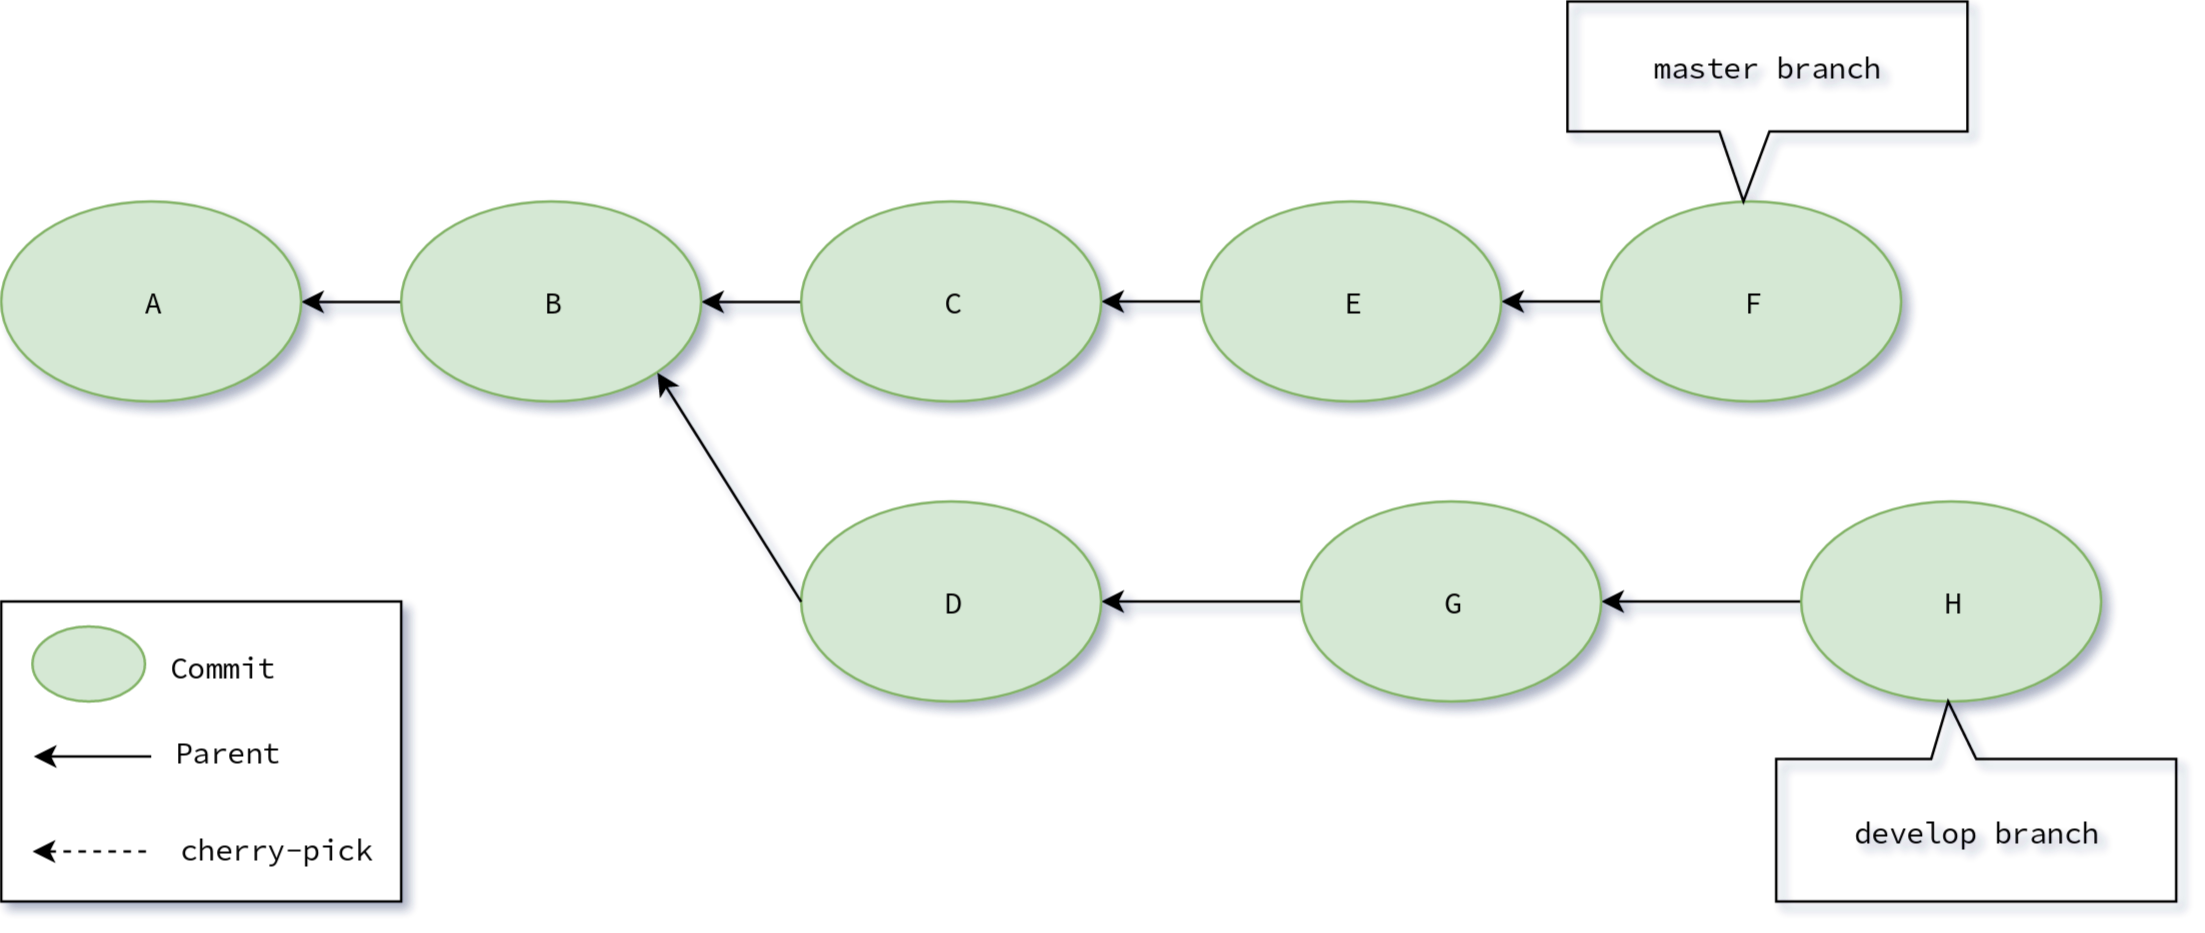
\includegraphics[width=1\textwidth,keepaspectratio]{./images/Rebase.png}
            }
            {
                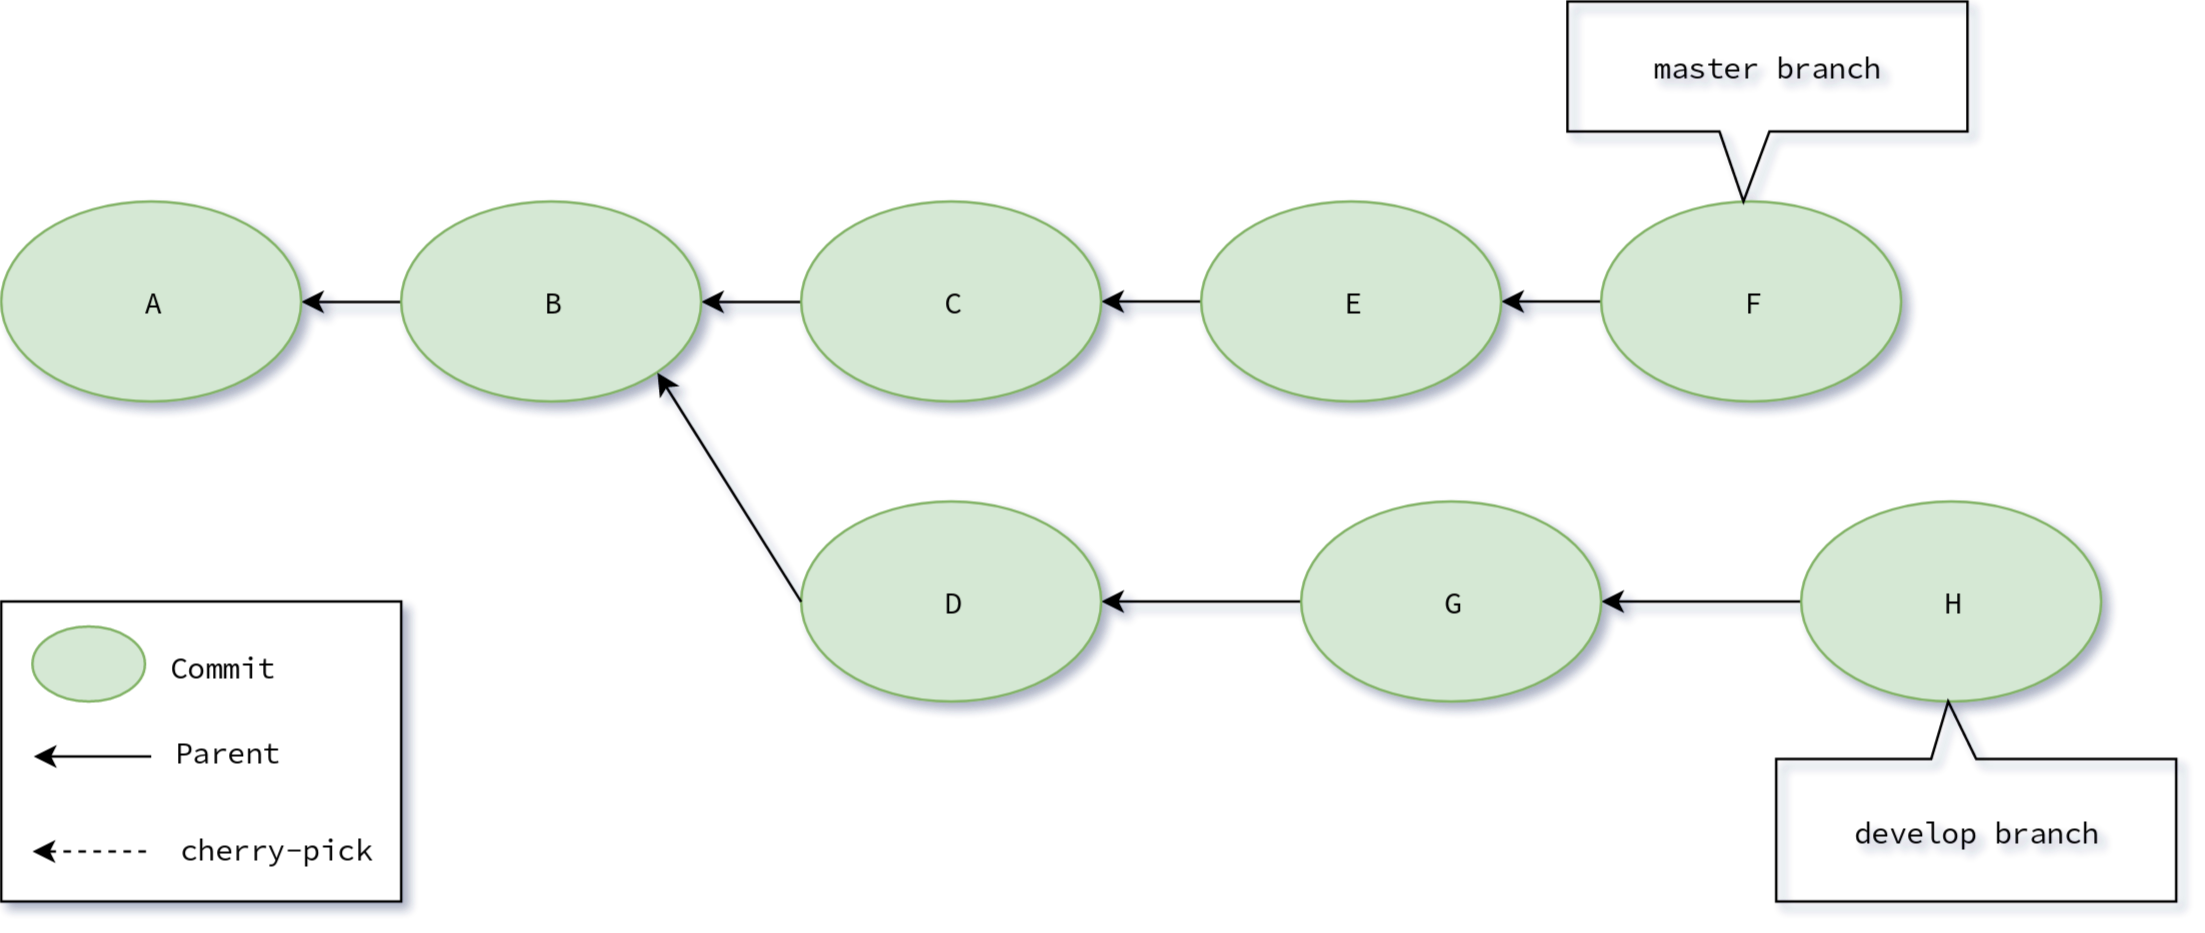
\includegraphics[height=0.75\textheight,keepaspectratio]{./images/Rebase.png}
            }
            \caption{Rebase scenario}
        \end{center}
    \end{figure}
\end{frame}

\begin{frame}[fragile]
    \frametitle{What does rebase do}
    \begin{figure}
        \begin{center}
            \ifnumequal{\aspectratio}{43}
            {
                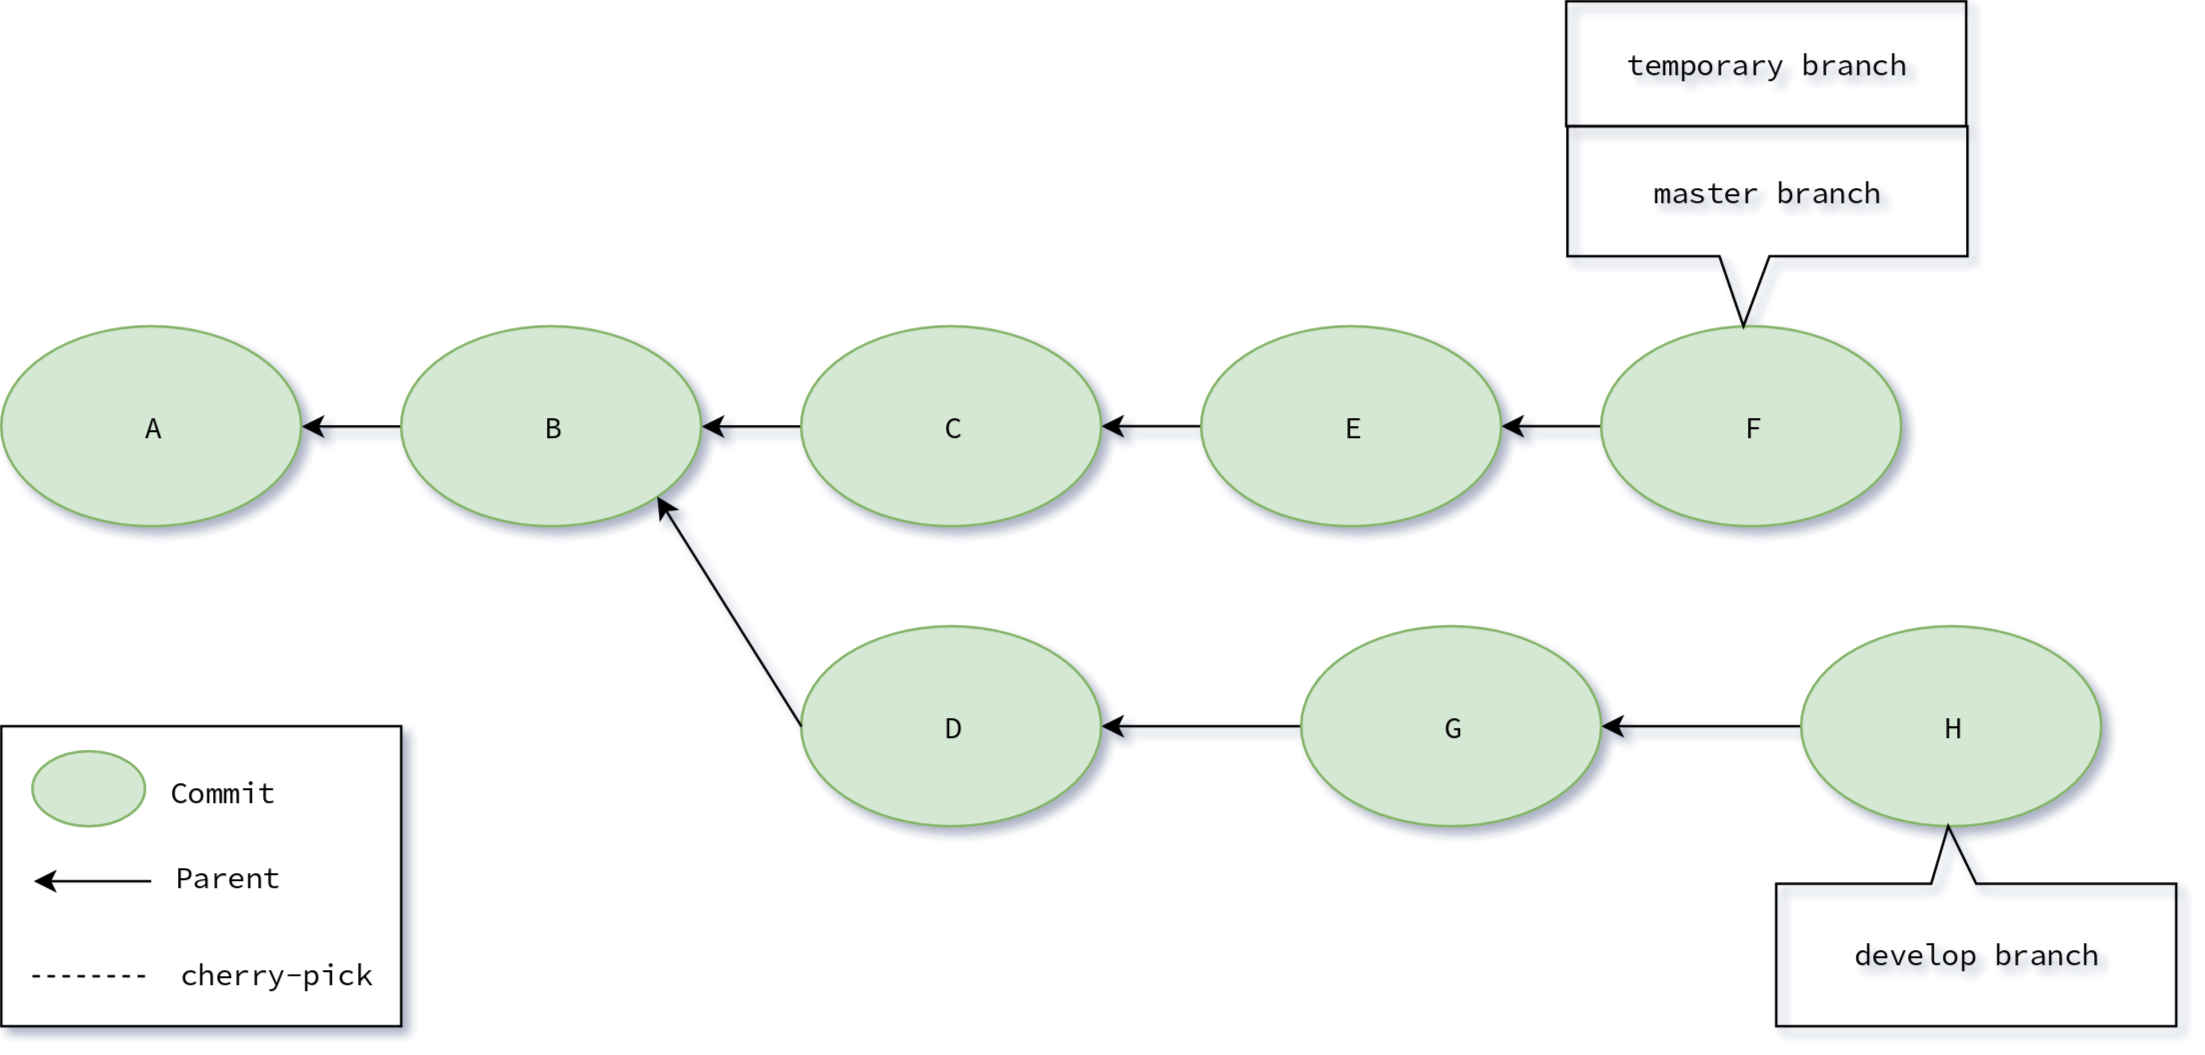
\includegraphics[width=1\textwidth,keepaspectratio]{./images/Rebase_TempBranch.png}
            }
            {
                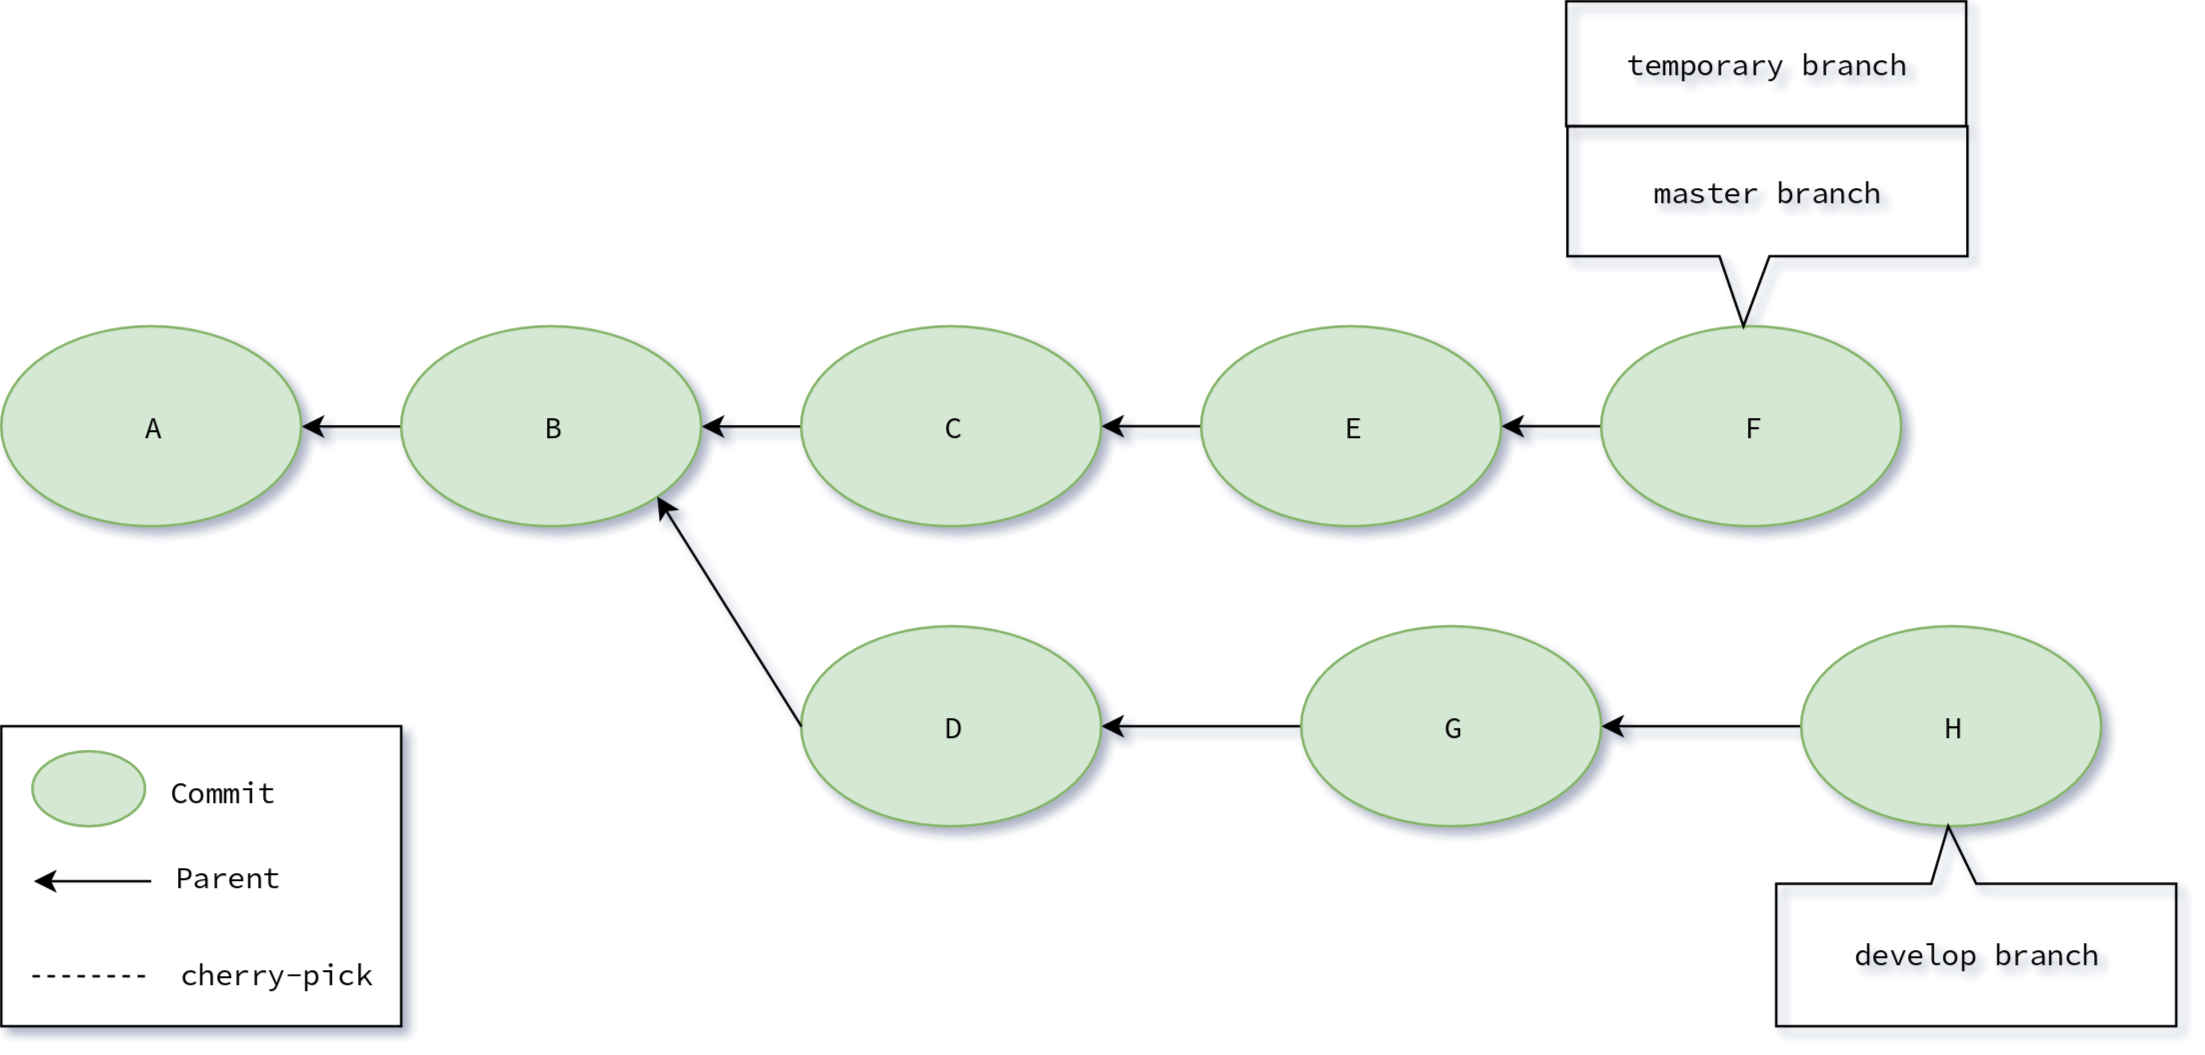
\includegraphics[height=0.75\textheight,keepaspectratio]{./images/Rebase_TempBranch.png}
            }
            \caption{Rebase temporary branch}
        \end{center}
    \end{figure}
\end{frame}

\begin{frame}[fragile]
    \frametitle{What does rebase do}
    \begin{figure}
        \begin{center}
            \ifnumequal{\aspectratio}{43}
            {
                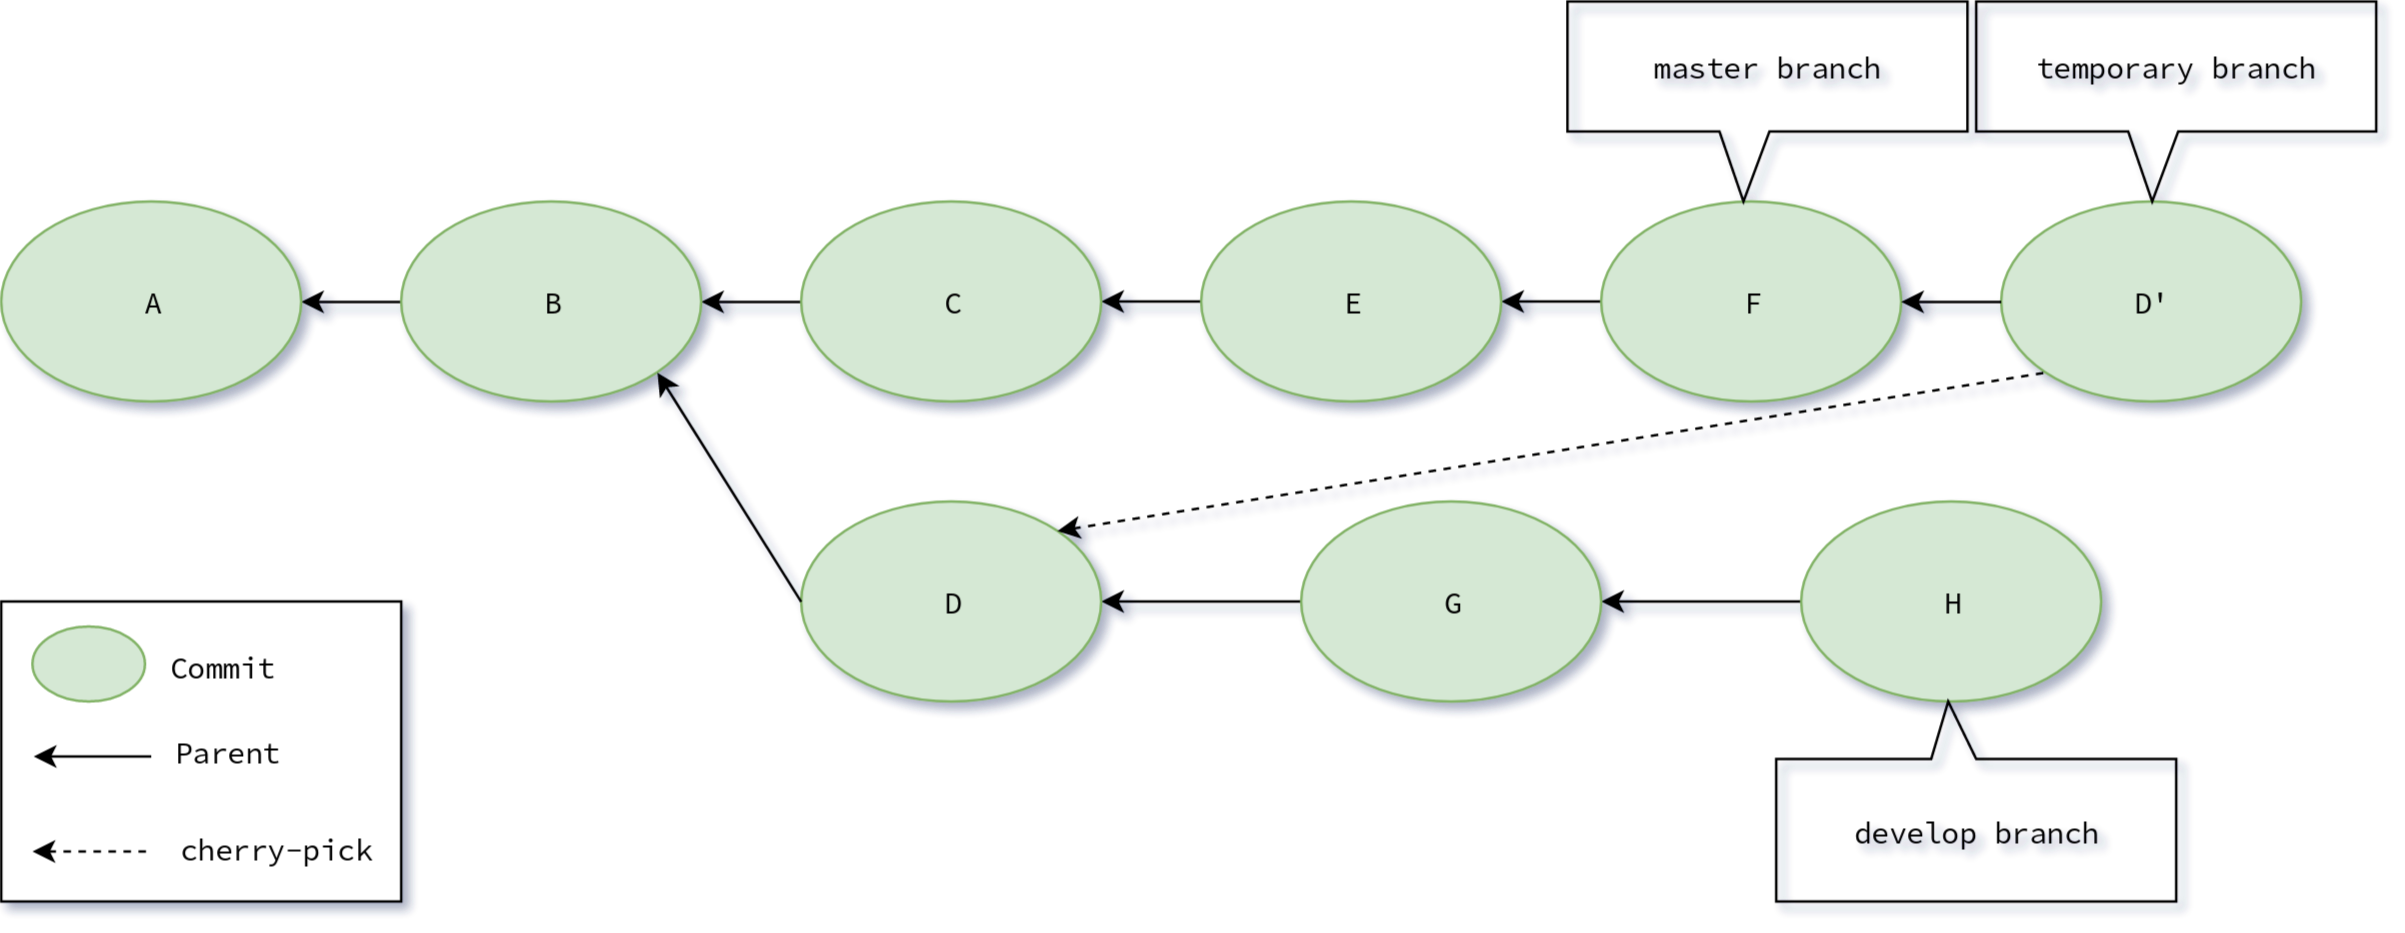
\includegraphics[width=1\textwidth,keepaspectratio]{./images/Rebase_FirstCherryPick.png}
            }
            {
                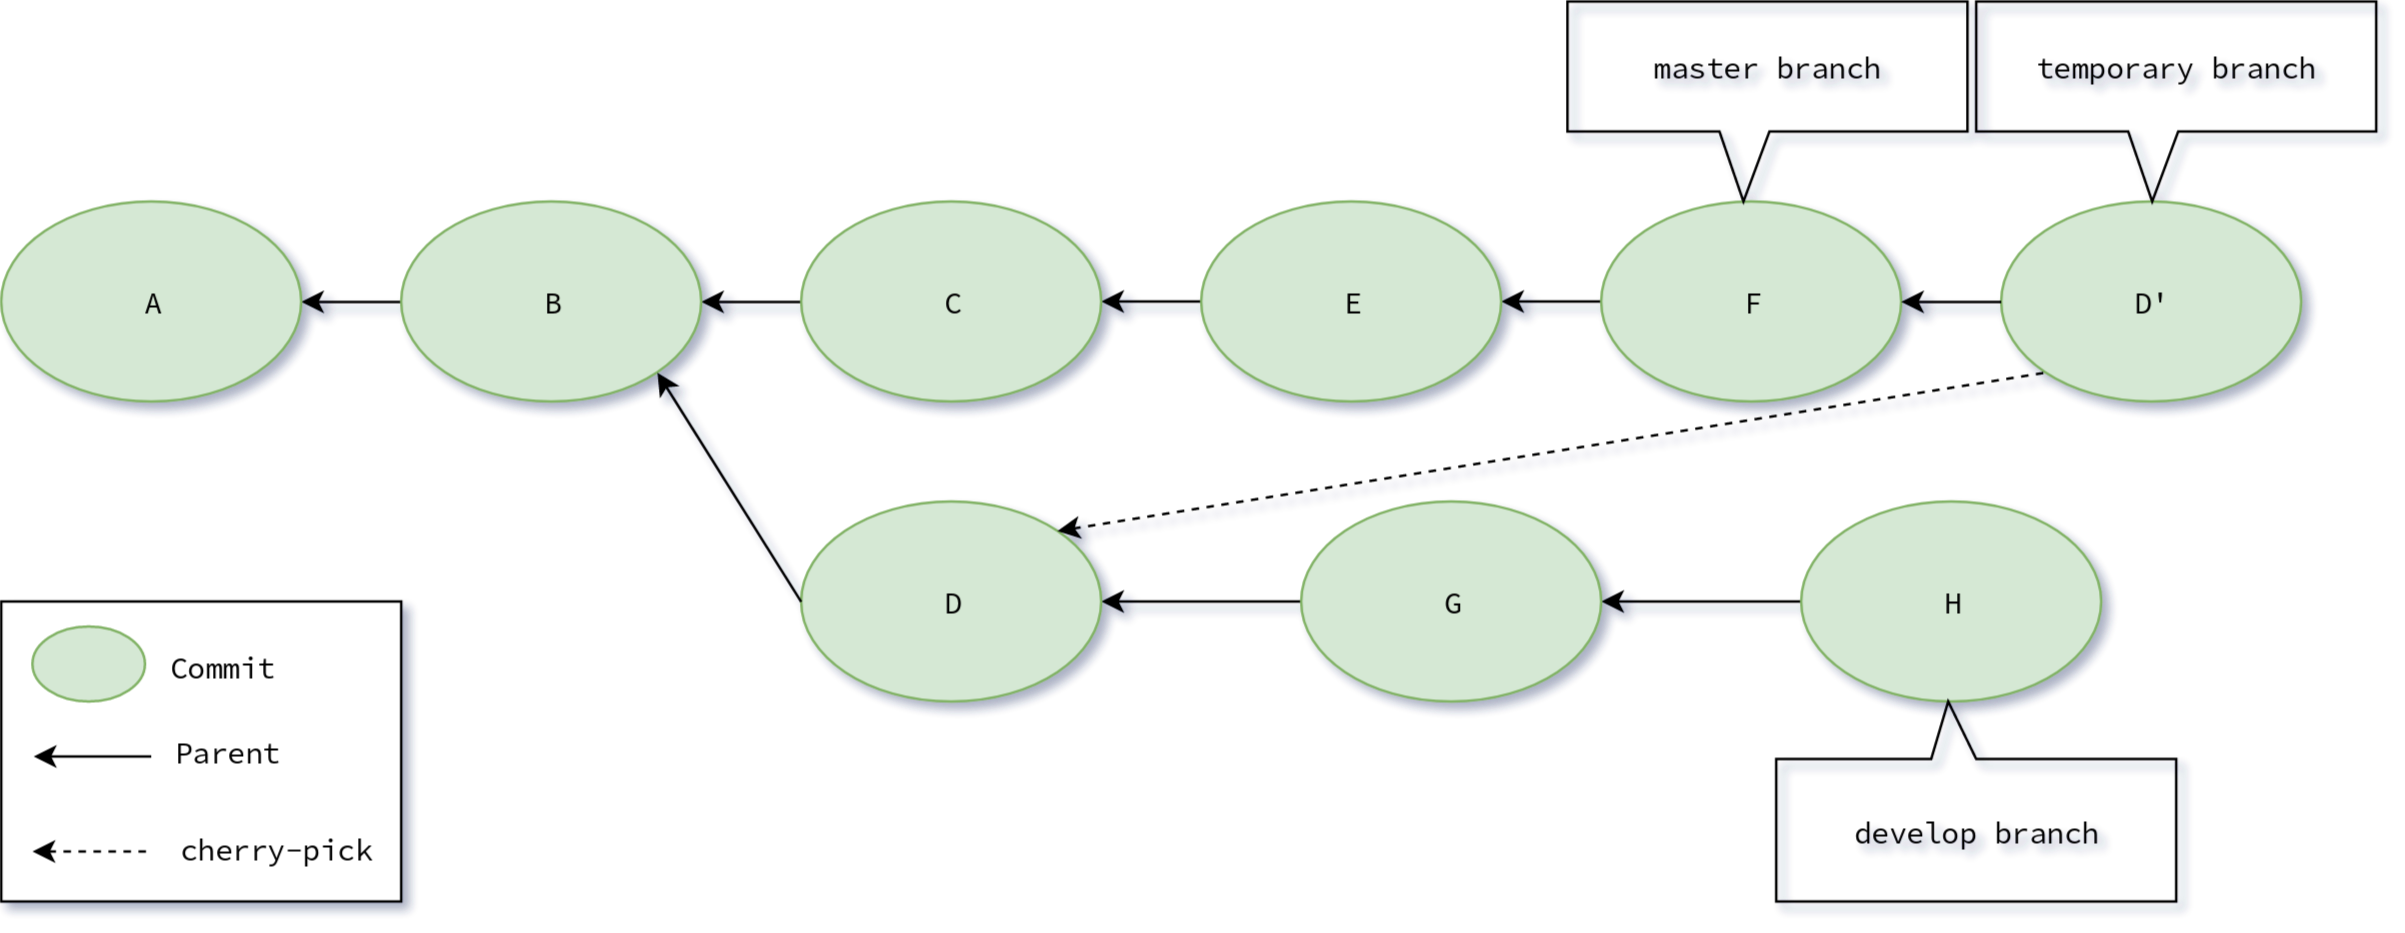
\includegraphics[width=0.9\textwidth,keepaspectratio]{./images/Rebase_FirstCherryPick.png}
            }
            \caption{Rebase first cherry-pick}
        \end{center}
    \end{figure}
\end{frame}

\begin{frame}[fragile]
    \frametitle{What does rebase do}
    \begin{figure}
        \begin{center}
            \ifnumequal{\aspectratio}{43}
            {
                \includegraphics[width=1\textwidth,keepaspectratio]{./images/Rebase-Process.png}
            }
            {
                \includegraphics[width=1\textwidth,keepaspectratio]{./images/Rebase-Process.png}
            }
            \caption{Rebase process cherry-picks}
        \end{center}
    \end{figure}
\end{frame}

\begin{frame}[fragile]
    \frametitle{What does rebase do}
    \begin{figure}
        \begin{center}
            \ifnumequal{\aspectratio}{43}
            {
                \includegraphics[width=1\textwidth,keepaspectratio]{./images/Rebase-Completed.png}
            }
            {
                \includegraphics[width=1\textwidth,keepaspectratio]{./images/Rebase-Completed.png}
            }
            \caption{Complete the rebase}
        \end{center}
    \end{figure}
\end{frame}



    \subsection{Recap}
\begin{frame}
    \frametitle{Cherry-pick recap}
    \begin{itemize}
        \item Only copies the content
        \item Metadata are copied
        \item Rebase uses cherry-pick
        \item Use \texttt{git rebase}/\texttt{git cherry-pick} in the right situations
    \end{itemize}
\end{frame}



    \section{Sources and further reading}
\begin{frame}[allowframebreaks]
    \frametitle{Sources and furhter reading}
    \begin{thebibliography}{10}
        \begin{columns}
            \column{0.4\textwidth}
            \beamertemplateonlinebibitems
            \bibitem{GitGuys}
            GitGuys
            \newblock {\em The Git Experts}.
            \newblock {\href{http://www.gitguys.com}{gitguys.com}}

            \beamertemplateonlinebibitems
            \bibitem{GitReady}
            GitReady
            \newblock {\em learn git one commit at a time}
            \newblock {\href{http://gitready.com}{gitready.com}}

            \beamertemplateonlinebibitems
            \bibitem{Draw io}
            Draw.io
            \newblock {\em Draw diagrams online}
            \newblock {\href{https://www.draw.io/}{draw.io}}

            \column{0.4\textwidth}
            \beamertemplateonlinebibitems
            \bibitem{Git manual}
            Git community (\href{https://github.com/schacon}{Scott Chacon})
            \newblock{\em Git manual reference}
            \newblock {\href{https://git-scm.com/docs}{git-scm.com/docs}}

            \beamertemplateonlinebibitems
            \bibitem{Git repository}
            Git Source Code Mirror
            \newblock{\em Git source code mirror}
            \newblock {\href{https://github.com/git/git/}{GitHub.com/git/git}}

            \beamertemplatearticlebibitems
            \bibitem{dotnetpro}
            German magazine for professional software developers
            \newblock{\em dotnetpro magazine}
            \newblock {\href{https://www.dotnetpro.de/}{dotnetpro.de}}
            \newblock {\href{https://www.dotnetpro.de/planung/ci-tools/deep-dive-git-1698582.html}{Deep Dive Git} 15.04.2019}
        \end{columns}

        \begin{columns}
            \column{0.4\textwidth}

            \beamertemplateonlinebibitems
            \bibitem{Git Cheatsheet}
            Git Cheatsheet
            \newblock{\em Interactive Git Cheatsheet from NDP software}
            \newblock {\href{https://ndpsoftware.com/git-cheatsheet.html}{Interactive Git Cheatsheet}}

            \beamertemplateonlinebibitems
            \bibitem{Git magic}
            Arthur C. Clarke
            \newblock {\em Reveals the magic of git}
            \newblock {
                \href{http://www-cs-students.stanford.edu/~blynn/gitmagic/index.html}
                    {www-cs-students.stanford.edu/{\textasciitilde}blynn/gitmagic}}
            \column{0.4\textwidth}

        \end{columns}
    \end{thebibliography}
\end{frame}



    \section*{Slides}
\begin{frame}[fragile]
    \frametitle{Slides and source}
    \begin{figure}
        \begin{center}
            \ifnumequal{\aspectratio}{43}
            {
                \includegraphics[height=0.6\textheight,keepaspectratio]{./images/qr_code.png}
            }
            {
                \includegraphics[height=0.6\textheight,keepaspectratio]{./images/qr_code.png}
            }
            \caption{GitHub repository for this presentation\footnotemark}
        \end{center}
    \end{figure}

    \footnotetext{
        \texttt{
            \href
                {https://github.com/vScherb/GitInternals}
                {https://github.com/vScherb/GitInternals}
        }
    }
\end{frame}


\end{document}

